\cajota{Población por sexo, según grupos de edad}{Para 2022, el grupo de edad de 0 a 4 años tuvo la población más grande de los grupos de edad con 1,870.5 miles de personas. El siguiente grupo más poblado fuel el de 5 a 9 años de edad con 1,864.1 miles de personas. Por el contrario,  la población de 100 años o más contó con la menor cantidad de personas de todos los grupos con 2.8 miles de personas. 

Las estimaciones indican que en los grupos quinquenales desde 0 hasta 24 años, predominaba la población de hombres. Sin embargo, en los grupos quinquenales a partir de los 25 años en adelante, predominaba la población de mujeres. Se estima que para 2022 hubo 277.0 miles de mujeres más que hombres.}{Población por sexo, según grupos de edad (miles de personas)}{República de Guatemala, Instituto Nacional de Estadística}{\begin{tikzpicture}[x=1pt,y=1pt, scale=1.75]% Created by tikzDevice version 0.12.4 on 2023-02-21 13:38:04
% !TEX encoding = UTF-8 Unicode
\definecolor{fillColor}{RGB}{255,255,255}
\path[use as bounding box,fill=fillColor,fill opacity=0.00] (0,0) rectangle (289.08,198.74);
\begin{scope}
\path[clip] (  0.00,  0.00) rectangle (289.08,198.74);

\path[] (  0.00,  0.00) rectangle (289.08,198.74);
\end{scope}
\begin{scope}
\path[clip] (  0.00,  0.00) rectangle (289.08,198.74);
\definecolor{drawColor}{RGB}{51,170,185}

\path[draw=drawColor,line width= 1.7pt,line join=round] ( 38.47, 83.93) --
	( 81.70, 93.46) --
	(124.92,105.02) --
	(168.15, 99.72) --
	(211.38,123.28) --
	(254.61,136.12);
\definecolor{drawColor}{RGB}{0,0,0}

\node[text=drawColor,anchor=base,inner sep=0pt, outer sep=0pt, scale=  1.02] at ( 38.47, 72.02) {479,120.8};

\node[text=drawColor,anchor=base east,inner sep=0pt, outer sep=0pt, scale=  1.02] at ( 74.55, 93.46) {495,443.9};

\node[text=drawColor,anchor=base,inner sep=0pt, outer sep=0pt, scale=  1.02] at (124.92,108.99) {515,273.1};

\node[text=drawColor,anchor=base,inner sep=0pt, outer sep=0pt, scale=  1.02] at (168.15, 87.81) {506,183.2};

\node[text=drawColor,anchor=base east,inner sep=0pt, outer sep=0pt, scale=  1.02] at (204.23,123.28) {546,580.6};

\node[text=drawColor,anchor=base,inner sep=0pt, outer sep=0pt, scale=  1.02] at (254.61,140.09) {568,578.8};

\path[draw=drawColor,line width= 0.1pt,line join=round] (-255.48, 26.12) -- (548.56, 26.12);

\path[] ( 12.53, 18.24) rectangle (280.54,191.48);

\path[] ( 12.53, 66.95) --
	(280.54, 66.95);

\path[] ( 12.53,125.28) --
	(280.54,125.28);

\path[] ( 12.53,183.61) --
	(280.54,183.61);

\path[] ( 12.53, 37.78) --
	(280.54, 37.78);

\path[] ( 12.53, 96.11) --
	(280.54, 96.11);

\path[] ( 12.53,154.44) --
	(280.54,154.44);

\path[] ( 38.47, 18.24) --
	( 38.47,191.48);

\path[] ( 81.70, 18.24) --
	( 81.70,191.48);

\path[] (124.92, 18.24) --
	(124.92,191.48);

\path[] (168.15, 18.24) --
	(168.15,191.48);

\path[] (211.38, 18.24) --
	(211.38,191.48);

\path[] (254.61, 18.24) --
	(254.61,191.48);

\path[] ( 12.53, 18.24) rectangle (280.54,191.48);
\end{scope}
\begin{scope}
\path[clip] (  0.00,  0.00) rectangle (289.08,198.74);

\path[] ( 12.53, 18.24) --
	( 12.53,191.48);
\end{scope}
\begin{scope}
\path[clip] (  0.00,  0.00) rectangle (289.08,198.74);
\definecolor{drawColor}{RGB}{255,255,255}

\node[text=drawColor,text opacity=0.00,anchor=base east,inner sep=0pt, outer sep=0pt, scale=  1.00] at (  7.58, 33.87) {4e+05};

\node[text=drawColor,text opacity=0.00,anchor=base east,inner sep=0pt, outer sep=0pt, scale=  1.00] at (  7.58, 92.20) {5e+05};

\node[text=drawColor,text opacity=0.00,anchor=base east,inner sep=0pt, outer sep=0pt, scale=  1.00] at (  7.58,150.53) {6e+05};
\end{scope}
\begin{scope}
\path[clip] (  0.00,  0.00) rectangle (289.08,198.74);

\path[] (  9.78, 37.78) --
	( 12.53, 37.78);

\path[] (  9.78, 96.11) --
	( 12.53, 96.11);

\path[] (  9.78,154.44) --
	( 12.53,154.44);
\end{scope}
\begin{scope}
\path[clip] (  0.00,  0.00) rectangle (289.08,198.74);

\path[] ( 12.53, 18.24) --
	(280.54, 18.24);
\end{scope}
\begin{scope}
\path[clip] (  0.00,  0.00) rectangle (289.08,198.74);

\path[] ( 38.47, 15.49) --
	( 38.47, 18.24);

\path[] ( 81.70, 15.49) --
	( 81.70, 18.24);

\path[] (124.92, 15.49) --
	(124.92, 18.24);

\path[] (168.15, 15.49) --
	(168.15, 18.24);

\path[] (211.38, 15.49) --
	(211.38, 18.24);

\path[] (254.61, 15.49) --
	(254.61, 18.24);
\end{scope}
\begin{scope}
\path[clip] (  0.00,  0.00) rectangle (289.08,198.74);
\definecolor{drawColor}{RGB}{0,0,0}

\node[text=drawColor,anchor=base,inner sep=0pt, outer sep=0pt, scale=  1.00] at ( 38.47,  4.16) {2017};

\node[text=drawColor,anchor=base,inner sep=0pt, outer sep=0pt, scale=  1.00] at ( 81.70,  4.16) {2018};

\node[text=drawColor,anchor=base,inner sep=0pt, outer sep=0pt, scale=  1.00] at (124.92,  4.16) {2019};

\node[text=drawColor,anchor=base,inner sep=0pt, outer sep=0pt, scale=  1.00] at (168.15,  4.16) {2020};

\node[text=drawColor,anchor=base,inner sep=0pt, outer sep=0pt, scale=  1.00] at (211.38,  4.16) {2021};

\node[text=drawColor,anchor=base,inner sep=0pt, outer sep=0pt, scale=  1.00] at (254.61,  4.16) {2022};
\end{scope}
\end{tikzpicture}}{INE - Censo 2018}

\cajita{Población por sexo, según dominio de estudio}{Para 2018, la mayoría de la población se encuentra en el área urbana son mujeres representando el 27.9\%. }{Población por sexo, según dominio de estudio (porcentaje)}{República de Guatemala, Instituto Nacional de Estadística}{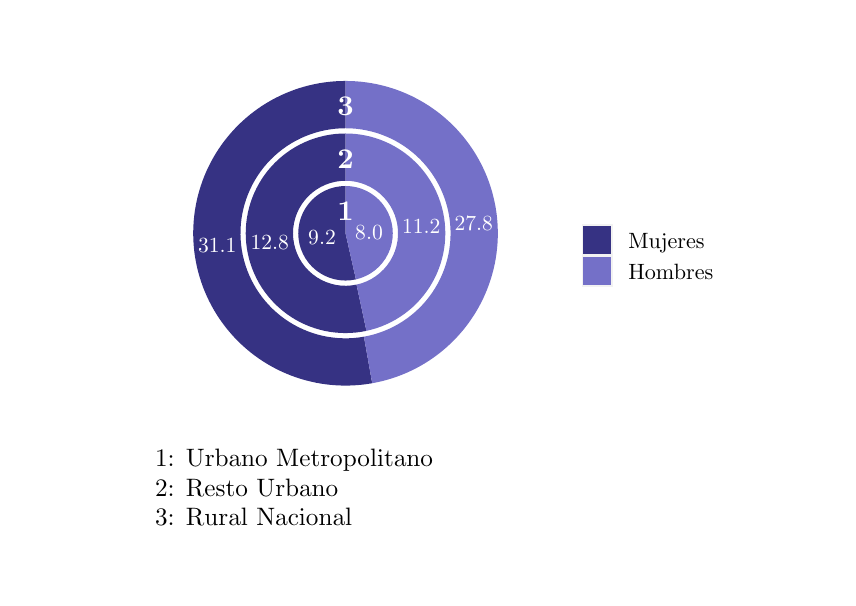
\begin{tikzpicture}[x=1pt,y=1pt]% Created by tikzDevice version 0.12.4 on 2023-05-05 09:28:13
% !TEX encoding = UTF-8 Unicode
\definecolor{fillColor}{RGB}{255,255,255}
\path[use as bounding box,fill=fillColor,fill opacity=0.00] (0,0) rectangle (289.08,198.74);
\begin{scope}
\path[clip] (  0.00,  0.00) rectangle (289.08,198.74);
\definecolor{drawColor}{RGB}{255,255,255}
\definecolor{fillColor}{RGB}{255,255,255}

\path[draw=drawColor,line width= 0.6pt,line join=round,line cap=round,fill=fillColor] ( 37.81,  0.00) rectangle (251.27,198.74);
\end{scope}
\begin{scope}
\path[clip] (  0.00,  0.00) rectangle (289.08,198.74);
\definecolor{fillColor}{RGB}{54,50,131}

\path[fill=fillColor] (114.85,124.45) --
	(114.85,126.34) --
	(114.85,128.24) --
	(114.85,130.14) --
	(114.85,132.04) --
	(114.85,133.93) --
	(114.85,135.83) --
	(114.85,137.73) --
	(114.85,139.63) --
	(114.85,141.53) --
	(112.94,141.42) --
	(111.06,141.10) --
	(109.22,140.57) --
	(107.45,139.84) --
	(105.77,138.91) --
	(104.21,137.81) --
	(102.78,136.53) --
	(101.51,135.10) --
	(100.40,133.54) --
	( 99.47,131.87) --
	( 98.74,130.10) --
	( 98.20,128.26) --
	( 97.88,126.38) --
	( 97.77,124.47) --
	( 97.88,122.56) --
	( 98.19,120.67) --
	( 98.72,118.83) --
	( 99.45,117.06) --
	(100.37,115.38) --
	(101.48,113.82) --
	(102.75,112.39) --
	(104.18,111.11) --
	(105.74,110.00) --
	(107.41,109.07) --
	(109.17,108.34) --
	(111.01,107.80) --
	(112.90,107.48) --
	(114.81,107.36) --
	(116.72,107.47) --
	(118.61,107.78) --
	(118.19,109.63) --
	(117.77,111.49) --
	(117.36,113.34) --
	(116.94,115.19) --
	(116.52,117.04) --
	(116.10,118.89) --
	(115.69,120.74) --
	(115.27,122.59) --
	(114.85,124.45) --
	(114.85,124.45) --
	cycle;

\path[fill=fillColor] (114.85,143.42) --
	(114.85,145.32) --
	(114.85,147.22) --
	(114.85,149.12) --
	(114.85,151.02) --
	(114.85,152.91) --
	(114.85,154.81) --
	(114.85,156.71) --
	(114.85,158.61) --
	(114.85,160.50) --
	(112.96,160.45) --
	(111.08,160.31) --
	(109.21,160.06) --
	(107.35,159.72) --
	(105.52,159.27) --
	(103.70,158.74) --
	(101.92,158.11) --
	(100.18,157.38) --
	( 98.48,156.57) --
	( 96.82,155.67) --
	( 95.21,154.68) --
	( 93.65,153.61) --
	( 92.15,152.46) --
	( 90.72,151.23) --
	( 89.35,149.93) --
	( 88.05,148.56) --
	( 86.82,147.13) --
	( 85.67,145.63) --
	( 84.60,144.07) --
	( 83.62,142.46) --
	( 82.72,140.80) --
	( 81.90,139.09) --
	( 81.18,137.35) --
	( 80.55,135.57) --
	( 80.02,133.76) --
	( 79.58,131.92) --
	( 79.23,130.06) --
	( 78.99,128.19) --
	( 78.84,126.31) --
	( 78.79,124.42) --
	( 78.84,122.53) --
	( 78.99,120.65) --
	( 79.24,118.77) --
	( 79.59,116.92) --
	( 80.03,115.08) --
	( 80.57,113.27) --
	( 81.20,111.49) --
	( 81.93,109.75) --
	( 82.74,108.04) --
	( 83.64,106.38) --
	( 84.63,104.77) --
	( 85.70,103.22) --
	( 86.85,101.72) --
	( 88.08,100.29) --
	( 89.38, 98.92) --
	( 90.76, 97.62) --
	( 92.19, 96.40) --
	( 93.69, 95.25) --
	( 95.25, 94.18) --
	( 96.86, 93.19) --
	( 98.52, 92.30) --
	(100.23, 91.48) --
	(101.98, 90.76) --
	(103.76, 90.14) --
	(105.57, 89.60) --
	(107.41, 89.16) --
	(109.26, 88.82) --
	(111.14, 88.58) --
	(113.02, 88.43) --
	(114.91, 88.39) --
	(116.80, 88.44) --
	(118.68, 88.59) --
	(120.55, 88.84) --
	(122.41, 89.19) --
	(122.01, 91.04) --
	(121.61, 92.90) --
	(121.21, 94.75) --
	(120.82, 96.61) --
	(120.42, 98.46) --
	(120.02,100.32) --
	(119.62,102.18) --
	(119.23,104.03) --
	(118.83,105.89) --
	(116.98,105.59) --
	(115.12,105.47) --
	(113.25,105.53) --
	(111.39,105.78) --
	(109.57,106.22) --
	(107.80,106.82) --
	(106.10,107.60) --
	(104.49,108.55) --
	(102.97,109.65) --
	(101.57,110.89) --
	(100.30,112.26) --
	( 99.17,113.75) --
	( 98.20,115.35) --
	( 97.38,117.03) --
	( 96.74,118.79) --
	( 96.27,120.60) --
	( 95.98,122.45) --
	( 95.87,124.31) --
	( 95.95,126.18) --
	( 96.22,128.03) --
	( 96.66,129.85) --
	( 97.28,131.62) --
	( 98.07,133.31) --
	( 99.03,134.92) --
	(100.14,136.43) --
	(101.39,137.82) --
	(102.77,139.08) --
	(104.27,140.20) --
	(105.87,141.16) --
	(107.56,141.97) --
	(109.32,142.60) --
	(111.13,143.06) --
	(112.98,143.33) --
	(114.85,143.42) --
	cycle;

\path[fill=fillColor] (114.85,162.40) --
	(114.85,164.30) --
	(114.85,166.20) --
	(114.85,168.10) --
	(114.85,169.99) --
	(114.85,171.89) --
	(114.85,173.79) --
	(114.85,175.69) --
	(114.85,177.59) --
	(114.85,179.48) --
	(112.99,179.45) --
	(111.13,179.36) --
	(109.27,179.20) --
	(107.42,178.98) --
	(105.58,178.70) --
	(103.75,178.35) --
	(101.93,177.94) --
	(100.13,177.48) --
	( 98.34,176.95) --
	( 96.57,176.36) --
	( 94.83,175.71) --
	( 93.10,175.00) --
	( 91.41,174.24) --
	( 89.73,173.42) --
	( 88.09,172.54) --
	( 86.48,171.60) --
	( 84.90,170.62) --
	( 83.35,169.58) --
	( 81.84,168.48) --
	( 80.37,167.34) --
	( 78.94,166.15) --
	( 77.55,164.91) --
	( 76.20,163.63) --
	( 74.90,162.29) --
	( 73.64,160.92) --
	( 72.43,159.50) --
	( 71.26,158.05) --
	( 70.15,156.55) --
	( 69.09,155.02) --
	( 68.08,153.46) --
	( 67.13,151.86) --
	( 66.23,150.22) --
	( 65.38,148.56) --
	( 64.59,146.88) --
	( 63.86,145.16) --
	( 63.19,143.42) --
	( 62.58,141.66) --
	( 62.03,139.89) --
	( 61.53,138.09) --
	( 61.10,136.28) --
	( 60.73,134.45) --
	( 60.42,132.61) --
	( 60.18,130.77) --
	( 60.00,128.91) --
	( 59.88,127.05) --
	( 59.82,125.19) --
	( 59.83,123.33) --
	( 59.90,121.46) --
	( 60.03,119.61) --
	( 60.22,117.75) --
	( 60.48,115.91) --
	( 60.80,114.07) --
	( 61.18,112.25) --
	( 61.63,110.44) --
	( 62.13,108.65) --
	( 62.70,106.87) --
	( 63.32,105.11) --
	( 64.01,103.38) --
	( 64.75,101.67) --
	( 65.55, 99.99) --
	( 66.40, 98.33) --
	( 67.31, 96.71) --
	( 68.28, 95.12) --
	( 69.30, 93.56) --
	( 70.37, 92.03) --
	( 71.49, 90.55) --
	( 72.67, 89.10) --
	( 73.89, 87.69) --
	( 75.15, 86.32) --
	( 76.47, 85.00) --
	( 77.82, 83.73) --
	( 79.22, 82.50) --
	( 80.66, 81.31) --
	( 82.14, 80.18) --
	( 83.66, 79.10) --
	( 85.21, 78.07) --
	( 86.80, 77.09) --
	( 88.42, 76.17) --
	( 90.07, 75.30) --
	( 91.74, 74.49) --
	( 93.45, 73.74) --
	( 95.18, 73.04) --
	( 96.93, 72.41) --
	( 98.70, 71.83) --
	(100.49, 71.31) --
	(102.30, 70.86) --
	(104.12, 70.46) --
	(105.95, 70.13) --
	(107.79, 69.86) --
	(109.65, 69.65) --
	(111.50, 69.51) --
	(113.36, 69.43) --
	(115.23, 69.41) --
	(117.09, 69.45) --
	(118.95, 69.56) --
	(120.81, 69.73) --
	(122.65, 69.96) --
	(124.49, 70.26) --
	(124.16, 72.13) --
	(123.83, 74.00) --
	(123.50, 75.86) --
	(123.16, 77.73) --
	(122.83, 79.60) --
	(122.50, 81.47) --
	(122.17, 83.34) --
	(121.83, 85.21) --
	(121.50, 87.07) --
	(119.64, 86.79) --
	(117.77, 86.60) --
	(115.90, 86.50) --
	(114.02, 86.50) --
	(112.14, 86.58) --
	(110.27, 86.77) --
	(108.41, 87.04) --
	(106.57, 87.40) --
	(104.74, 87.86) --
	(102.95, 88.40) --
	(101.18, 89.04) --
	( 99.44, 89.76) --
	( 97.74, 90.56) --
	( 96.09, 91.45) --
	( 94.48, 92.42) --
	( 92.92, 93.47) --
	( 91.41, 94.59) --
	( 89.96, 95.79) --
	( 88.57, 97.06) --
	( 87.25, 98.39) --
	( 85.99, 99.79) --
	( 84.81,101.25) --
	( 83.70,102.76) --
	( 82.66,104.33) --
	( 81.71,105.95) --
	( 80.83,107.61) --
	( 80.04,109.32) --
	( 79.33,111.06) --
	( 78.72,112.83) --
	( 78.18,114.64) --
	( 77.74,116.46) --
	( 77.39,118.31) --
	( 77.14,120.17) --
	( 76.97,122.04) --
	( 76.90,123.92) --
	( 76.92,125.80) --
	( 77.03,127.68) --
	( 77.24,129.55) --
	( 77.54,131.40) --
	( 77.93,133.24) --
	( 78.41,135.06) --
	( 78.98,136.85) --
	( 79.64,138.61) --
	( 80.38,140.33) --
	( 81.21,142.02) --
	( 82.12,143.66) --
	( 83.11,145.26) --
	( 84.18,146.81) --
	( 85.33,148.30) --
	( 86.54,149.73) --
	( 87.83,151.10) --
	( 89.18,152.40) --
	( 90.60,153.64) --
	( 92.07,154.81) --
	( 93.60,155.90) --
	( 95.19,156.91) --
	( 96.82,157.84) --
	( 98.49,158.69) --
	(100.21,159.46) --
	(101.96,160.14) --
	(103.74,160.74) --
	(105.55,161.24) --
	(107.38,161.66) --
	(109.23,161.98) --
	(111.10,162.22) --
	(112.97,162.36) --
	(114.85,162.40) --
	cycle;
\definecolor{fillColor}{RGB}{116,112,200}

\path[fill=fillColor] (114.85,124.45) --
	(115.27,122.59) --
	(115.69,120.74) --
	(116.10,118.89) --
	(116.52,117.04) --
	(116.94,115.19) --
	(117.36,113.34) --
	(117.77,111.49) --
	(118.19,109.63) --
	(118.61,107.78) --
	(120.45,108.31) --
	(122.23,109.04) --
	(123.91,109.96) --
	(125.47,111.07) --
	(126.90,112.34) --
	(128.18,113.77) --
	(129.30,115.33) --
	(130.23,117.01) --
	(130.97,118.77) --
	(131.50,120.62) --
	(131.82,122.51) --
	(131.93,124.42) --
	(131.83,126.33) --
	(131.51,128.22) --
	(130.98,130.07) --
	(130.25,131.84) --
	(129.32,133.52) --
	(128.22,135.08) --
	(126.94,136.51) --
	(125.51,137.79) --
	(123.95,138.90) --
	(122.27,139.83) --
	(120.50,140.57) --
	(118.66,141.10) --
	(116.77,141.42) --
	(114.85,141.53) --
	(114.85,139.63) --
	(114.85,137.73) --
	(114.85,135.83) --
	(114.85,133.93) --
	(114.85,132.04) --
	(114.85,130.14) --
	(114.85,128.24) --
	(114.85,126.34) --
	(114.85,124.45) --
	(114.85,124.45) --
	cycle;

\path[fill=fillColor] (118.83,105.89) --
	(119.23,104.03) --
	(119.62,102.18) --
	(120.02,100.32) --
	(120.42, 98.46) --
	(120.82, 96.61) --
	(121.21, 94.75) --
	(121.61, 92.90) --
	(122.01, 91.04) --
	(122.41, 89.19) --
	(124.24, 89.63) --
	(126.05, 90.17) --
	(127.83, 90.80) --
	(129.57, 91.53) --
	(131.27, 92.34) --
	(132.93, 93.24) --
	(134.53, 94.23) --
	(136.09, 95.30) --
	(137.58, 96.45) --
	(139.02, 97.68) --
	(140.38, 98.98) --
	(141.68,100.35) --
	(142.90,101.79) --
	(144.05,103.29) --
	(145.12,104.84) --
	(146.10,106.45) --
	(147.00,108.11) --
	(147.81,109.81) --
	(148.53,111.56) --
	(149.16,113.34) --
	(149.69,115.15) --
	(150.13,116.98) --
	(150.47,118.84) --
	(150.72,120.71) --
	(150.86,122.59) --
	(150.91,124.48) --
	(150.86,126.36) --
	(150.71,128.24) --
	(150.46,130.11) --
	(150.12,131.97) --
	(149.68,133.80) --
	(149.14,135.61) --
	(148.51,137.39) --
	(147.79,139.13) --
	(146.97,140.84) --
	(146.07,142.49) --
	(145.08,144.10) --
	(144.01,145.66) --
	(142.87,147.15) --
	(141.64,148.59) --
	(140.34,149.95) --
	(138.97,151.25) --
	(137.54,152.48) --
	(136.04,153.62) --
	(134.48,154.69) --
	(132.87,155.68) --
	(131.22,156.58) --
	(129.51,157.39) --
	(127.77,158.11) --
	(125.99,158.74) --
	(124.18,159.28) --
	(122.35,159.72) --
	(120.49,160.06) --
	(118.62,160.31) --
	(116.74,160.46) --
	(114.85,160.50) --
	(114.85,158.61) --
	(114.85,156.71) --
	(114.85,154.81) --
	(114.85,152.91) --
	(114.85,151.02) --
	(114.85,149.12) --
	(114.85,147.22) --
	(114.85,145.32) --
	(114.85,143.42) --
	(116.77,143.33) --
	(118.66,143.04) --
	(120.52,142.56) --
	(122.32,141.89) --
	(124.04,141.05) --
	(125.67,140.04) --
	(127.19,138.87) --
	(128.58,137.55) --
	(129.83,136.10) --
	(130.93,134.53) --
	(131.87,132.86) --
	(132.63,131.10) --
	(133.21,129.27) --
	(133.60,127.39) --
	(133.80,125.49) --
	(133.81,123.57) --
	(133.63,121.66) --
	(133.25,119.78) --
	(132.69,117.95) --
	(131.94,116.19) --
	(131.02,114.50) --
	(129.93,112.92) --
	(128.69,111.46) --
	(127.31,110.13) --
	(125.81,108.95) --
	(124.19,107.92) --
	(122.47,107.06) --
	(120.68,106.38) --
	(118.83,105.89) --
	cycle;

\path[fill=fillColor] (121.50, 87.07) --
	(121.83, 85.21) --
	(122.17, 83.34) --
	(122.50, 81.47) --
	(122.83, 79.60) --
	(123.16, 77.73) --
	(123.50, 75.86) --
	(123.83, 74.00) --
	(124.16, 72.13) --
	(124.49, 70.26) --
	(126.34, 70.62) --
	(128.16, 71.04) --
	(129.98, 71.53) --
	(131.77, 72.07) --
	(133.54, 72.68) --
	(135.30, 73.35) --
	(137.03, 74.07) --
	(138.73, 74.86) --
	(140.41, 75.70) --
	(142.05, 76.60) --
	(143.67, 77.55) --
	(145.25, 78.56) --
	(146.80, 79.63) --
	(148.31, 80.74) --
	(149.78, 81.91) --
	(151.20, 83.12) --
	(152.59, 84.38) --
	(153.94, 85.69) --
	(155.23, 87.05) --
	(156.48, 88.44) --
	(157.69, 89.88) --
	(158.84, 91.36) --
	(159.94, 92.88) --
	(160.99, 94.44) --
	(161.99, 96.03) --
	(162.93, 97.65) --
	(163.81, 99.30) --
	(164.64,100.99) --
	(165.41,102.70) --
	(166.12,104.43) --
	(166.78,106.19) --
	(167.37,107.97) --
	(167.90,109.77) --
	(168.37,111.59) --
	(168.78,113.42) --
	(169.12,115.26) --
	(169.40,117.12) --
	(169.62,118.98) --
	(169.77,120.85) --
	(169.86,122.72) --
	(169.89,124.60) --
	(169.85,126.48) --
	(169.75,128.35) --
	(169.59,130.22) --
	(169.36,132.08) --
	(169.07,133.93) --
	(168.71,135.78) --
	(168.29,137.60) --
	(167.82,139.42) --
	(167.27,141.21) --
	(166.67,142.99) --
	(166.01,144.75) --
	(165.29,146.48) --
	(164.51,148.18) --
	(163.67,149.86) --
	(162.78,151.51) --
	(161.83,153.13) --
	(160.82,154.71) --
	(159.76,156.26) --
	(158.65,157.77) --
	(157.49,159.25) --
	(156.28,160.68) --
	(155.02,162.07) --
	(153.72,163.42) --
	(152.36,164.72) --
	(150.97,165.97) --
	(149.53,167.18) --
	(148.06,168.34) --
	(146.54,169.44) --
	(144.99,170.50) --
	(143.40,171.50) --
	(141.78,172.44) --
	(140.13,173.33) --
	(138.45,174.17) --
	(136.74,174.94) --
	(135.01,175.66) --
	(133.25,176.32) --
	(131.47,176.91) --
	(129.68,177.45) --
	(127.86,177.92) --
	(126.03,178.34) --
	(124.19,178.69) --
	(122.33,178.97) --
	(120.47,179.20) --
	(118.60,179.36) --
	(116.73,179.45) --
	(114.85,179.48) --
	(114.85,177.59) --
	(114.85,175.69) --
	(114.85,173.79) --
	(114.85,171.89) --
	(114.85,169.99) --
	(114.85,168.10) --
	(114.85,166.20) --
	(114.85,164.30) --
	(114.85,162.40) --
	(116.73,162.36) --
	(118.60,162.22) --
	(120.46,161.99) --
	(122.31,161.66) --
	(124.14,161.25) --
	(125.94,160.75) --
	(127.72,160.15) --
	(129.47,159.47) --
	(131.19,158.71) --
	(132.86,157.86) --
	(134.49,156.93) --
	(136.07,155.92) --
	(137.60,154.83) --
	(139.07,153.67) --
	(140.49,152.44) --
	(141.84,151.14) --
	(143.12,149.77) --
	(144.34,148.35) --
	(145.48,146.86) --
	(146.55,145.32) --
	(147.55,143.73) --
	(148.46,142.09) --
	(149.29,140.41) --
	(150.04,138.69) --
	(150.70,136.93) --
	(151.27,135.14) --
	(151.76,133.33) --
	(152.15,131.50) --
	(152.45,129.65) --
	(152.66,127.78) --
	(152.78,125.91) --
	(152.81,124.03) --
	(152.74,122.16) --
	(152.58,120.29) --
	(152.33,118.43) --
	(151.99,116.59) --
	(151.55,114.76) --
	(151.03,112.96) --
	(150.42,111.19) --
	(149.72,109.45) --
	(148.94,107.74) --
	(148.07,106.08) --
	(147.12,104.46) --
	(146.10,102.89) --
	(144.99,101.37) --
	(143.82, 99.91) --
	(142.57, 98.51) --
	(141.25, 97.17) --
	(139.87, 95.90) --
	(138.43, 94.70) --
	(136.94, 93.57) --
	(135.38, 92.52) --
	(133.78, 91.54) --
	(132.13, 90.65) --
	(130.44, 89.84) --
	(128.71, 89.11) --
	(126.95, 88.47) --
	(125.16, 87.91) --
	(123.34, 87.45) --
	(121.50, 87.07) --
	cycle;
\definecolor{drawColor}{RGB}{255,255,255}

\node[text=drawColor,anchor=base,inner sep=0pt, outer sep=0pt, scale=  0.78] at (106.36,120.47) {9.2};

\node[text=drawColor,anchor=base,inner sep=0pt, outer sep=0pt, scale=  0.78] at ( 87.49,118.51) {12.8};

\node[text=drawColor,anchor=base,inner sep=0pt, outer sep=0pt, scale=  0.78] at ( 68.54,117.32) {31.1};

\node[text=drawColor,anchor=base,inner sep=0pt, outer sep=0pt, scale=  0.78] at (123.34,122.36) {8.0};

\node[text=drawColor,anchor=base,inner sep=0pt, outer sep=0pt, scale=  0.78] at (142.22,124.31) {11.2};

\node[text=drawColor,anchor=base,inner sep=0pt, outer sep=0pt, scale=  0.78] at (161.17,125.50) {27.8};

\node[text=drawColor,anchor=base,inner sep=0pt, outer sep=0pt, scale=  1.03] at (114.85,128.94) {\bfseries 1};

\node[text=drawColor,anchor=base,inner sep=0pt, outer sep=0pt, scale=  1.03] at (114.85,147.92) {\bfseries 2};

\node[text=drawColor,anchor=base,inner sep=0pt, outer sep=0pt, scale=  1.03] at (114.85,166.90) {\bfseries 3};
\end{scope}
\begin{scope}
\path[clip] (  0.00,  0.00) rectangle (289.08,198.74);
\definecolor{fillColor}{RGB}{255,255,255}

\path[fill=fillColor] (194.65, 99.59) rectangle (245.77,149.30);
\end{scope}
\begin{scope}
\path[clip] (  0.00,  0.00) rectangle (289.08,198.74);
\definecolor{fillColor}{gray}{0.95}

\path[fill=fillColor] (200.15,116.47) rectangle (211.53,127.85);
\end{scope}
\begin{scope}
\path[clip] (  0.00,  0.00) rectangle (289.08,198.74);
\definecolor{fillColor}{RGB}{54,50,131}

\path[fill=fillColor] (200.81,117.13) rectangle (210.87,127.19);
\end{scope}
\begin{scope}
\path[clip] (  0.00,  0.00) rectangle (289.08,198.74);
\definecolor{fillColor}{gray}{0.95}

\path[fill=fillColor] (200.15,105.09) rectangle (211.53,116.47);
\end{scope}
\begin{scope}
\path[clip] (  0.00,  0.00) rectangle (289.08,198.74);
\definecolor{fillColor}{RGB}{116,112,200}

\path[fill=fillColor] (200.81,105.75) rectangle (210.87,115.81);
\end{scope}
\begin{scope}
\path[clip] (  0.00,  0.00) rectangle (289.08,198.74);
\definecolor{drawColor}{RGB}{0,0,0}

\node[text=drawColor,anchor=base west,inner sep=0pt, outer sep=0pt, scale=  0.80] at (217.03,119.04) {Mujeres};
\end{scope}
\begin{scope}
\path[clip] (  0.00,  0.00) rectangle (289.08,198.74);
\definecolor{drawColor}{RGB}{0,0,0}

\node[text=drawColor,anchor=base west,inner sep=0pt, outer sep=0pt, scale=  0.80] at (217.03,107.65) {Hombres};
\end{scope}
\begin{scope}
\path[clip] (  0.00,  0.00) rectangle (289.08,198.74);
\definecolor{drawColor}{RGB}{0,0,0}

\node[text=drawColor,anchor=base west,inner sep=0pt, outer sep=0pt, scale=  0.91] at ( 46.06, 40.29) {1: Urbano Metropolitano};

\node[text=drawColor,anchor=base west,inner sep=0pt, outer sep=0pt, scale=  0.91] at ( 46.06, 29.49) {2: Resto Urbano};

\node[text=drawColor,anchor=base west,inner sep=0pt, outer sep=0pt, scale=  0.91] at ( 46.06, 18.69) {3: Rural Nacional};

\node[text=drawColor,anchor=base west,inner sep=0pt, outer sep=0pt, scale=  0.91] at ( 46.06,  7.89) {};
\end{scope}
\end{tikzpicture}}{INE - ENEI 2022}{}

\cajita{Población por sexo, según Pueblos}{Para 2022, el 31.2\% de la población guatemalteca estaba compuesta por mujeres ladinas. El 27.8\% eran hombres ladinos, y el 19.6\% mujeres mayas. El 0.1\% eran mujeres garífunas, otro 0.1\% hombres garífunas, y 0.1\% mujeres extranjeras. \footnote{Afrodescendiente*: Afrodescendiente/Creole/Afro mestizo.}}{Población por sexo, según Pueblos (porcentaje)}{República de Guatemala, Instituto Nacional de Estadística}{\begin{tikzpicture}[x=1pt,y=1pt]% Created by tikzDevice version 0.12.4 on 2023-04-17 10:12:35
% !TEX encoding = UTF-8 Unicode
\definecolor{fillColor}{RGB}{255,255,255}
\path[use as bounding box,fill=fillColor,fill opacity=0.00] (0,0) rectangle (289.08,198.74);
\begin{scope}
\path[clip] (  0.00,  0.00) rectangle (289.08,198.74);

\path[] (  0.00,  0.00) rectangle (289.08,198.74);
\end{scope}
\begin{scope}
\path[clip] (  0.00,  0.00) rectangle (289.08,198.74);
\definecolor{fillColor}{RGB}{54,50,131}

\path[fill=fillColor] (  8.16, 21.09) rectangle ( 26.81, 24.65);

\path[fill=fillColor] ( 54.79, 21.09) rectangle ( 73.44, 21.65);

\path[fill=fillColor] (101.41, 21.09) rectangle (120.06,170.58);

\path[fill=fillColor] (148.04, 21.09) rectangle (166.69, 27.18);

\path[fill=fillColor] (194.66, 21.09) rectangle (213.31, 21.56);

\path[fill=fillColor] (241.29, 21.09) rectangle (259.94,115.07);
\definecolor{fillColor}{RGB}{116,112,200}

\path[fill=fillColor] ( 29.14, 21.09) rectangle ( 47.79, 23.99);

\path[fill=fillColor] ( 75.77, 21.09) rectangle ( 94.42, 21.55);

\path[fill=fillColor] (122.39, 21.09) rectangle (141.04,154.24);

\path[fill=fillColor] (169.02, 21.09) rectangle (187.67, 27.61);

\path[fill=fillColor] (215.64, 21.09) rectangle (234.29, 21.81);

\path[fill=fillColor] (262.27, 21.09) rectangle (280.92,102.16);
\definecolor{drawColor}{RGB}{0,0,0}

\path[draw=drawColor,line width= 0.6pt,line join=round] (-289.08, 21.09) -- (578.16, 21.09);

\node[text=drawColor,anchor=base,inner sep=0pt, outer sep=0pt, scale=  0.83] at ( 17.48, 27.88) {0.7};

\node[text=drawColor,anchor=base,inner sep=0pt, outer sep=0pt, scale=  0.83] at ( 64.11, 24.88) {0.1};

\node[text=drawColor,anchor=base,inner sep=0pt, outer sep=0pt, scale=  0.83] at (110.74,173.81) {31.2};

\node[text=drawColor,anchor=base,inner sep=0pt, outer sep=0pt, scale=  0.83] at (157.36, 30.41) {1.3};

\node[text=drawColor,anchor=base,inner sep=0pt, outer sep=0pt, scale=  0.83] at (203.99, 24.80) {0.1};

\node[text=drawColor,anchor=base,inner sep=0pt, outer sep=0pt, scale=  0.83] at (250.61,118.30) {19.6};

\node[text=drawColor,anchor=base,inner sep=0pt, outer sep=0pt, scale=  0.83] at ( 38.47, 27.22) {0.6};

\node[text=drawColor,anchor=base,inner sep=0pt, outer sep=0pt, scale=  0.83] at ( 85.09, 24.78) {0.1};

\node[text=drawColor,anchor=base,inner sep=0pt, outer sep=0pt, scale=  0.83] at (131.72,157.48) {27.8};

\node[text=drawColor,anchor=base,inner sep=0pt, outer sep=0pt, scale=  0.83] at (178.34, 30.85) {1.4};

\node[text=drawColor,anchor=base,inner sep=0pt, outer sep=0pt, scale=  0.83] at (224.97, 25.04) {0.2};

\node[text=drawColor,anchor=base,inner sep=0pt, outer sep=0pt, scale=  0.83] at (271.60,105.40) {16.9};

\path[] (  0.00, 21.09) rectangle (289.08,170.58);

\path[] ( 27.98, 21.09) --
	( 27.98,170.58);

\path[] ( 74.60, 21.09) --
	( 74.60,170.58);

\path[] (121.23, 21.09) --
	(121.23,170.58);

\path[] (167.85, 21.09) --
	(167.85,170.58);

\path[] (214.48, 21.09) --
	(214.48,170.58);

\path[] (261.10, 21.09) --
	(261.10,170.58);

\path[] (  0.00, 21.09) rectangle (289.08,170.58);
\end{scope}
\begin{scope}
\path[clip] (  0.00,  0.00) rectangle (289.08,198.74);

\path[] (  0.00, 21.09) --
	(  0.00,170.58);
\end{scope}
\begin{scope}
\path[clip] (  0.00,  0.00) rectangle (289.08,198.74);

\path[] (  0.00, 21.09) --
	(289.08, 21.09);
\end{scope}
\begin{scope}
\path[clip] (  0.00,  0.00) rectangle (289.08,198.74);

\path[] ( 27.98, 18.34) --
	( 27.98, 21.09);

\path[] ( 74.60, 18.34) --
	( 74.60, 21.09);

\path[] (121.23, 18.34) --
	(121.23, 21.09);

\path[] (167.85, 18.34) --
	(167.85, 21.09);

\path[] (214.48, 18.34) --
	(214.48, 21.09);

\path[] (261.10, 18.34) --
	(261.10, 21.09);
\end{scope}
\begin{scope}
\path[clip] (  0.00,  0.00) rectangle (289.08,198.74);
\definecolor{drawColor}{RGB}{0,0,0}

\node[text=drawColor,anchor=base,inner sep=0pt, outer sep=0pt, scale=  1.00] at ( 27.98,  7.01) {Xinka};

\node[text=drawColor,anchor=base,inner sep=0pt, outer sep=0pt, scale=  1.00] at ( 74.60,  7.01) {Garífuna};

\node[text=drawColor,anchor=base,inner sep=0pt, outer sep=0pt, scale=  1.00] at (121.23,  7.01) {Ladino};

\node[text=drawColor,anchor=base,inner sep=0pt, outer sep=0pt, scale=  1.00] at (167.85,  7.01) {Afrodescendiente*};

\node[text=drawColor,anchor=base,inner sep=0pt, outer sep=0pt, scale=  1.00] at (214.48,  7.01) {Extranjero};

\node[text=drawColor,anchor=base,inner sep=0pt, outer sep=0pt, scale=  1.00] at (261.10,  7.01) {Maya};
\end{scope}
\begin{scope}
\path[clip] (  0.00,  0.00) rectangle (289.08,198.74);
\coordinate (apoyo) at (55.92,189.21);
\coordinate (longitudFicticia) at (7.11,9.53);
\coordinate (longitud) at (7.11,7.11);
\coordinate (desX) at (137.28,0);
\coordinate (desY) at (0,1.21);
\definecolor[named]{ct1}{HTML}{
363283
}
\definecolor[named]{ct2}{HTML}{
7470C8
}
\definecolor[named]{ctb1}{HTML}{
363283
}
\definecolor[named]{ctb2}{HTML}{
7470C8
}
\path [fill=none] (apoyo) rectangle ($(apoyo)+(longitudFicticia)$)
node [xshift=0.3cm,inner sep=0pt, outer sep=0pt,midway,right,scale = 0.9]{Mujeres};
\draw [color = ctb1,fill=ct1] ( $(apoyo)  + (desY) $) rectangle ($(apoyo)+ (desY) +(longitud)$);
\path [fill=none] ($(apoyo)+(desX)$) rectangle ($(apoyo)+(desX)+(longitudFicticia)$)
node [xshift=0.3cm,inner sep=0pt, outer sep=0pt,midway,right,scale = 0.9]{Hombres};
\draw [color = ctb2 ,fill=ct2] ( $(apoyo)  + (desY) + (desX) $) rectangle ($(apoyo)+ (desY)+ (desX) +(longitud)$);
\end{scope}
\end{tikzpicture}}{INE - ENEI 2022}{}

\cajota{Población por sexo, según comunidad lingüística}{Para el 2018, se muestra el número de personas por sexo pertenecientes a cada comunidad lingüística Maya. Se observa que en la mayoría de comunidades existe una mayor población de mujeres, con excepción de la comunidad Itza'.  }{Población por sexo, según comunidad lingüística (número de personas)}{República de Guatemala, Instituto Nacional de Estadística}{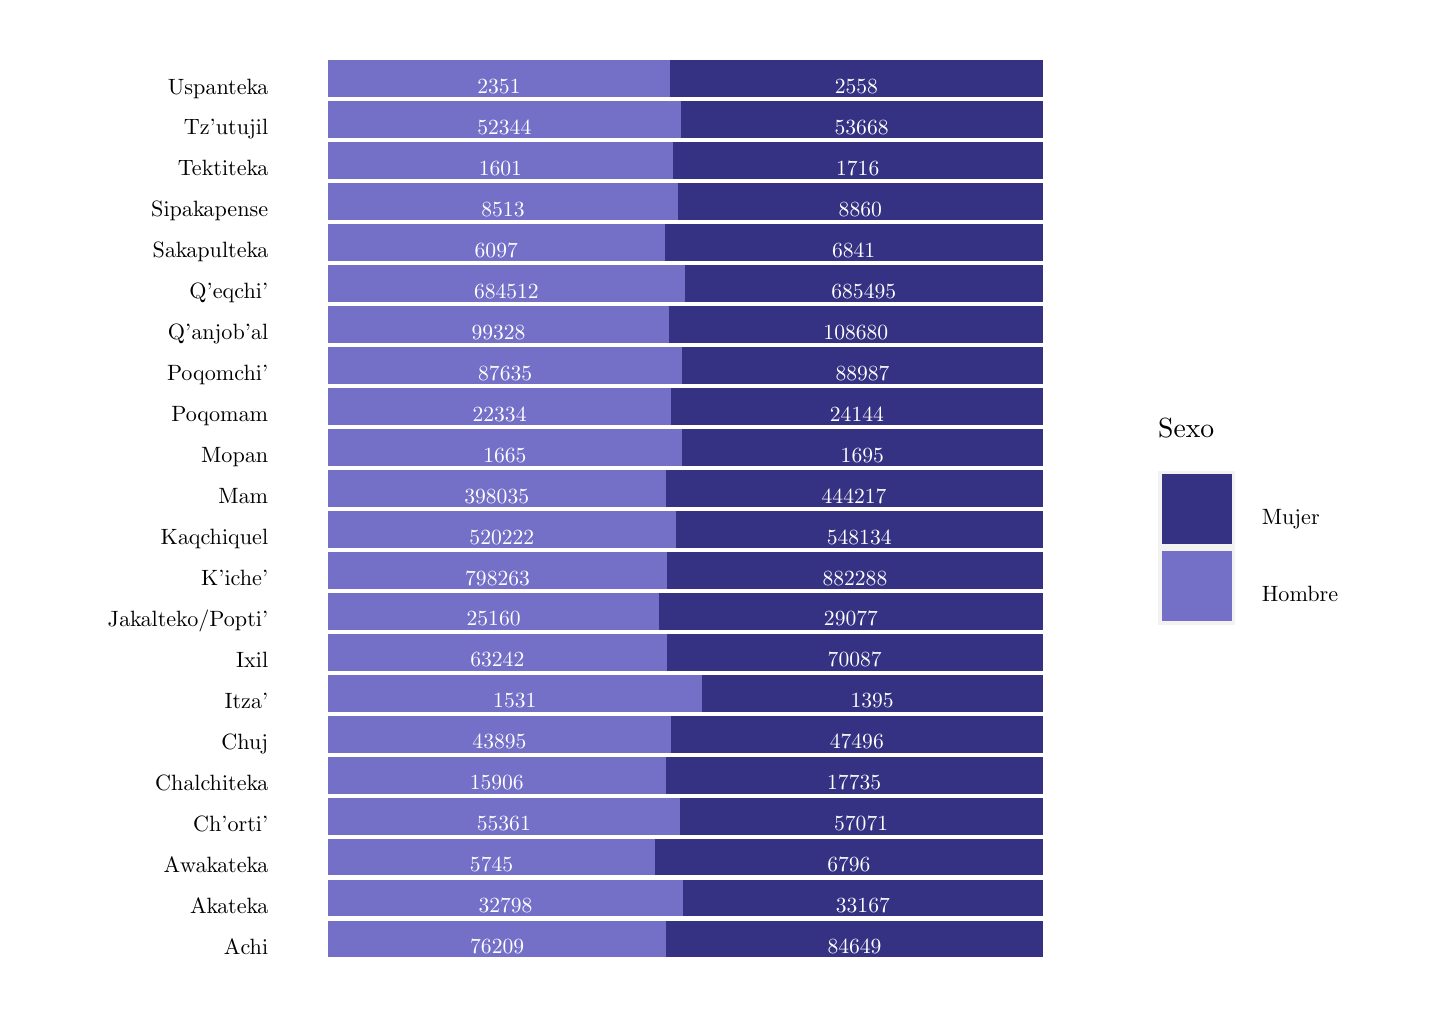
\begin{tikzpicture}[x=1pt,y=1pt, scale=1.75]% Created by tikzDevice version 0.12.4 on 2023-04-20 09:23:04
% !TEX encoding = UTF-8 Unicode
\definecolor{fillColor}{RGB}{255,255,255}
\path[use as bounding box,fill=fillColor,fill opacity=0.00] (0,0) rectangle (289.08,198.74);
\begin{scope}
\path[clip] (  0.00,  0.00) rectangle (289.08,198.74);
\definecolor{drawColor}{RGB}{255,255,255}
\definecolor{fillColor}{RGB}{255,255,255}

\path[draw=drawColor,line width= 0.6pt,line join=round,line cap=round,fill=fillColor] (  0.00,  0.00) rectangle (289.08,198.74);
\end{scope}
\begin{scope}
\path[clip] (  0.00,  0.00) rectangle (289.08,198.74);
\definecolor{fillColor}{RGB}{54,50,131}

\path[fill=fillColor] (131.90,  6.77) rectangle (209.56, 14.38);

\path[fill=fillColor] (135.36, 15.23) rectangle (209.56, 22.84);

\path[fill=fillColor] (129.59, 23.68) rectangle (209.56, 31.29);

\path[fill=fillColor] (134.65, 32.14) rectangle (209.56, 39.75);

\path[fill=fillColor] (131.76, 40.60) rectangle (209.56, 48.21);

\path[fill=fillColor] (132.86, 49.05) rectangle (209.56, 56.66);

\path[fill=fillColor] (139.20, 57.51) rectangle (209.56, 65.12);

\path[fill=fillColor] (131.98, 65.97) rectangle (209.56, 73.58);

\path[fill=fillColor] (130.44, 74.42) rectangle (209.56, 82.03);

\path[fill=fillColor] (132.08, 82.88) rectangle (209.56, 90.49);

\path[fill=fillColor] (133.84, 91.34) rectangle (209.56, 98.95);

\path[fill=fillColor] (131.73, 99.79) rectangle (209.56,107.41);

\path[fill=fillColor] (135.11,108.25) rectangle (209.56,115.86);

\path[fill=fillColor] (132.90,116.71) rectangle (209.56,124.32);

\path[fill=fillColor] (135.21,125.16) rectangle (209.56,132.78);

\path[fill=fillColor] (132.45,133.62) rectangle (209.56,141.23);

\path[fill=fillColor] (135.72,142.08) rectangle (209.56,149.69);

\path[fill=fillColor] (131.53,150.54) rectangle (209.56,158.15);

\path[fill=fillColor] (134.30,158.99) rectangle (209.56,166.60);

\path[fill=fillColor] (133.21,167.45) rectangle (209.56,175.06);

\path[fill=fillColor] (134.85,175.91) rectangle (209.56,183.52);

\path[fill=fillColor] (132.66,184.36) rectangle (209.56,191.97);
\definecolor{fillColor}{RGB}{116,112,200}

\path[fill=fillColor] ( 61.98,  6.77) rectangle (131.90, 14.38);

\path[fill=fillColor] ( 61.98, 15.23) rectangle (135.36, 22.84);

\path[fill=fillColor] ( 61.98, 23.68) rectangle (129.59, 31.29);

\path[fill=fillColor] ( 61.98, 32.14) rectangle (134.65, 39.75);

\path[fill=fillColor] ( 61.98, 40.60) rectangle (131.76, 48.21);

\path[fill=fillColor] ( 61.98, 49.05) rectangle (132.86, 56.66);

\path[fill=fillColor] ( 61.98, 57.51) rectangle (139.20, 65.12);

\path[fill=fillColor] ( 61.98, 65.97) rectangle (131.98, 73.58);

\path[fill=fillColor] ( 61.98, 74.42) rectangle (130.44, 82.03);

\path[fill=fillColor] ( 61.98, 82.88) rectangle (132.08, 90.49);

\path[fill=fillColor] ( 61.98, 91.34) rectangle (133.84, 98.95);

\path[fill=fillColor] ( 61.98, 99.79) rectangle (131.73,107.41);

\path[fill=fillColor] ( 61.98,108.25) rectangle (135.11,115.86);

\path[fill=fillColor] ( 61.98,116.71) rectangle (132.90,124.32);

\path[fill=fillColor] ( 61.98,125.16) rectangle (135.21,132.78);

\path[fill=fillColor] ( 61.98,133.62) rectangle (132.45,141.23);

\path[fill=fillColor] ( 61.98,142.08) rectangle (135.72,149.69);

\path[fill=fillColor] ( 61.98,150.54) rectangle (131.53,158.15);

\path[fill=fillColor] ( 61.98,158.99) rectangle (134.30,166.60);

\path[fill=fillColor] ( 61.98,167.45) rectangle (133.21,175.06);

\path[fill=fillColor] ( 61.98,175.91) rectangle (134.85,183.52);

\path[fill=fillColor] ( 61.98,184.36) rectangle (132.66,191.97);
\definecolor{drawColor}{RGB}{255,255,255}

\node[text=drawColor,anchor=base,inner sep=0pt, outer sep=0pt, scale=  0.78] at (170.73,  7.54) {84649};

\node[text=drawColor,anchor=base,inner sep=0pt, outer sep=0pt, scale=  0.78] at (172.46, 16.00) {33167};

\node[text=drawColor,anchor=base,inner sep=0pt, outer sep=0pt, scale=  0.78] at (169.57, 24.45) {6796};

\node[text=drawColor,anchor=base,inner sep=0pt, outer sep=0pt, scale=  0.78] at (172.10, 32.91) {57071};

\node[text=drawColor,anchor=base,inner sep=0pt, outer sep=0pt, scale=  0.78] at (170.66, 41.37) {17735};

\node[text=drawColor,anchor=base,inner sep=0pt, outer sep=0pt, scale=  0.78] at (171.21, 49.83) {47496};

\node[text=drawColor,anchor=base,inner sep=0pt, outer sep=0pt, scale=  0.78] at (174.38, 58.28) {1395};

\node[text=drawColor,anchor=base,inner sep=0pt, outer sep=0pt, scale=  0.78] at (170.77, 66.74) {70087};

\node[text=drawColor,anchor=base,inner sep=0pt, outer sep=0pt, scale=  0.78] at (170.00, 75.20) {29077};

\node[text=drawColor,anchor=base,inner sep=0pt, outer sep=0pt, scale=  0.78] at (170.82, 83.65) {882288};

\node[text=drawColor,anchor=base,inner sep=0pt, outer sep=0pt, scale=  0.78] at (171.70, 92.11) {548134};

\node[text=drawColor,anchor=base,inner sep=0pt, outer sep=0pt, scale=  0.78] at (170.64,100.57) {444217};

\node[text=drawColor,anchor=base,inner sep=0pt, outer sep=0pt, scale=  0.78] at (172.34,109.02) {1695};

\node[text=drawColor,anchor=base,inner sep=0pt, outer sep=0pt, scale=  0.78] at (171.23,117.48) {24144};

\node[text=drawColor,anchor=base,inner sep=0pt, outer sep=0pt, scale=  0.78] at (172.38,125.94) {88987};

\node[text=drawColor,anchor=base,inner sep=0pt, outer sep=0pt, scale=  0.78] at (171.01,134.39) {108680};

\node[text=drawColor,anchor=base,inner sep=0pt, outer sep=0pt, scale=  0.78] at (172.64,142.85) {685495};

\node[text=drawColor,anchor=base,inner sep=0pt, outer sep=0pt, scale=  0.78] at (170.54,151.31) {6841};

\node[text=drawColor,anchor=base,inner sep=0pt, outer sep=0pt, scale=  0.78] at (171.93,159.76) {8860};

\node[text=drawColor,anchor=base,inner sep=0pt, outer sep=0pt, scale=  0.78] at (171.39,168.22) {1716};

\node[text=drawColor,anchor=base,inner sep=0pt, outer sep=0pt, scale=  0.78] at (172.20,176.68) {53668};

\node[text=drawColor,anchor=base,inner sep=0pt, outer sep=0pt, scale=  0.78] at (171.11,185.14) {2558};

\node[text=drawColor,anchor=base,inner sep=0pt, outer sep=0pt, scale=  0.78] at ( 96.94,  7.54) {76209};

\node[text=drawColor,anchor=base,inner sep=0pt, outer sep=0pt, scale=  0.78] at ( 98.67, 16.00) {32798};

\node[text=drawColor,anchor=base,inner sep=0pt, outer sep=0pt, scale=  0.78] at ( 95.79, 24.45) {5745};

\node[text=drawColor,anchor=base,inner sep=0pt, outer sep=0pt, scale=  0.78] at ( 98.32, 32.91) {55361};

\node[text=drawColor,anchor=base,inner sep=0pt, outer sep=0pt, scale=  0.78] at ( 96.87, 41.37) {15906};

\node[text=drawColor,anchor=base,inner sep=0pt, outer sep=0pt, scale=  0.78] at ( 97.42, 49.83) {43895};

\node[text=drawColor,anchor=base,inner sep=0pt, outer sep=0pt, scale=  0.78] at (100.59, 58.28) {1531};

\node[text=drawColor,anchor=base,inner sep=0pt, outer sep=0pt, scale=  0.78] at ( 96.98, 66.74) {63242};

\node[text=drawColor,anchor=base,inner sep=0pt, outer sep=0pt, scale=  0.78] at ( 96.21, 75.20) {25160};

\node[text=drawColor,anchor=base,inner sep=0pt, outer sep=0pt, scale=  0.78] at ( 97.03, 83.65) {798263};

\node[text=drawColor,anchor=base,inner sep=0pt, outer sep=0pt, scale=  0.78] at ( 97.91, 92.11) {520222};

\node[text=drawColor,anchor=base,inner sep=0pt, outer sep=0pt, scale=  0.78] at ( 96.85,100.57) {398035};

\node[text=drawColor,anchor=base,inner sep=0pt, outer sep=0pt, scale=  0.78] at ( 98.55,109.02) {1665};

\node[text=drawColor,anchor=base,inner sep=0pt, outer sep=0pt, scale=  0.78] at ( 97.44,117.48) {22334};

\node[text=drawColor,anchor=base,inner sep=0pt, outer sep=0pt, scale=  0.78] at ( 98.60,125.94) {87635};

\node[text=drawColor,anchor=base,inner sep=0pt, outer sep=0pt, scale=  0.78] at ( 97.22,134.39) {99328};

\node[text=drawColor,anchor=base,inner sep=0pt, outer sep=0pt, scale=  0.78] at ( 98.85,142.85) {684512};

\node[text=drawColor,anchor=base,inner sep=0pt, outer sep=0pt, scale=  0.78] at ( 96.76,151.31) {6097};

\node[text=drawColor,anchor=base,inner sep=0pt, outer sep=0pt, scale=  0.78] at ( 98.14,159.76) {8513};

\node[text=drawColor,anchor=base,inner sep=0pt, outer sep=0pt, scale=  0.78] at ( 97.60,168.22) {1601};

\node[text=drawColor,anchor=base,inner sep=0pt, outer sep=0pt, scale=  0.78] at ( 98.42,176.68) {52344};

\node[text=drawColor,anchor=base,inner sep=0pt, outer sep=0pt, scale=  0.78] at ( 97.32,185.14) {2351};
\end{scope}
\begin{scope}
\path[clip] (  0.00,  0.00) rectangle (289.08,198.74);
\definecolor{drawColor}{RGB}{0,0,0}

\node[text=drawColor,anchor=base east,inner sep=0pt, outer sep=0pt, scale=  0.80] at ( 49.66,  7.45) {Achi};

\node[text=drawColor,anchor=base east,inner sep=0pt, outer sep=0pt, scale=  0.80] at ( 49.66, 15.90) {Akateka};

\node[text=drawColor,anchor=base east,inner sep=0pt, outer sep=0pt, scale=  0.80] at ( 49.66, 24.36) {Awakateka};

\node[text=drawColor,anchor=base east,inner sep=0pt, outer sep=0pt, scale=  0.80] at ( 49.66, 32.82) {Ch'orti'};

\node[text=drawColor,anchor=base east,inner sep=0pt, outer sep=0pt, scale=  0.80] at ( 49.66, 41.27) {Chalchiteka};

\node[text=drawColor,anchor=base east,inner sep=0pt, outer sep=0pt, scale=  0.80] at ( 49.66, 49.73) {Chuj};

\node[text=drawColor,anchor=base east,inner sep=0pt, outer sep=0pt, scale=  0.80] at ( 49.66, 58.19) {Itza'};

\node[text=drawColor,anchor=base east,inner sep=0pt, outer sep=0pt, scale=  0.80] at ( 49.66, 66.65) {Ixil};

\node[text=drawColor,anchor=base east,inner sep=0pt, outer sep=0pt, scale=  0.80] at ( 49.66, 75.10) {Jakalteko/Popti'};

\node[text=drawColor,anchor=base east,inner sep=0pt, outer sep=0pt, scale=  0.80] at ( 49.66, 83.56) {K'iche'};

\node[text=drawColor,anchor=base east,inner sep=0pt, outer sep=0pt, scale=  0.80] at ( 49.66, 92.02) {Kaqchiquel};

\node[text=drawColor,anchor=base east,inner sep=0pt, outer sep=0pt, scale=  0.80] at ( 49.66,100.47) {Mam};

\node[text=drawColor,anchor=base east,inner sep=0pt, outer sep=0pt, scale=  0.80] at ( 49.66,108.93) {Mopan};

\node[text=drawColor,anchor=base east,inner sep=0pt, outer sep=0pt, scale=  0.80] at ( 49.66,117.39) {Poqomam};

\node[text=drawColor,anchor=base east,inner sep=0pt, outer sep=0pt, scale=  0.80] at ( 49.66,125.84) {Poqomchi'};

\node[text=drawColor,anchor=base east,inner sep=0pt, outer sep=0pt, scale=  0.80] at ( 49.66,134.30) {Q'anjob'al};

\node[text=drawColor,anchor=base east,inner sep=0pt, outer sep=0pt, scale=  0.80] at ( 49.66,142.76) {Q'eqchi'};

\node[text=drawColor,anchor=base east,inner sep=0pt, outer sep=0pt, scale=  0.80] at ( 49.66,151.21) {Sakapulteka};

\node[text=drawColor,anchor=base east,inner sep=0pt, outer sep=0pt, scale=  0.80] at ( 49.66,159.67) {Sipakapense};

\node[text=drawColor,anchor=base east,inner sep=0pt, outer sep=0pt, scale=  0.80] at ( 49.66,168.13) {Tektiteka};

\node[text=drawColor,anchor=base east,inner sep=0pt, outer sep=0pt, scale=  0.80] at ( 49.66,176.58) {Tz'utujil};

\node[text=drawColor,anchor=base east,inner sep=0pt, outer sep=0pt, scale=  0.80] at ( 49.66,185.04) {Uspanteka};
\end{scope}
\begin{scope}
\path[clip] (  0.00,  0.00) rectangle (289.08,198.74);
\definecolor{fillColor}{RGB}{255,255,255}

\path[fill=fillColor] (227.94, 69.99) rectangle (283.58,128.75);
\end{scope}
\begin{scope}
\path[clip] (  0.00,  0.00) rectangle (289.08,198.74);
\definecolor{drawColor}{RGB}{0,0,0}

\node[text=drawColor,anchor=base west,inner sep=0pt, outer sep=0pt, scale=  1.00] at (233.44,114.11) {Sexo};
\end{scope}
\begin{scope}
\path[clip] (  0.00,  0.00) rectangle (289.08,198.74);
\definecolor{fillColor}{gray}{0.95}

\path[fill=fillColor] (233.44, 91.39) rectangle (249.34,107.29);
\end{scope}
\begin{scope}
\path[clip] (  0.00,  0.00) rectangle (289.08,198.74);
\definecolor{fillColor}{RGB}{54,50,131}

\path[fill=fillColor] (234.15, 92.10) rectangle (248.63,106.58);
\end{scope}
\begin{scope}
\path[clip] (  0.00,  0.00) rectangle (289.08,198.74);
\definecolor{fillColor}{gray}{0.95}

\path[fill=fillColor] (233.44, 75.49) rectangle (249.34, 91.39);
\end{scope}
\begin{scope}
\path[clip] (  0.00,  0.00) rectangle (289.08,198.74);
\definecolor{fillColor}{RGB}{116,112,200}

\path[fill=fillColor] (234.15, 76.20) rectangle (248.63, 90.68);
\end{scope}
\begin{scope}
\path[clip] (  0.00,  0.00) rectangle (289.08,198.74);
\definecolor{drawColor}{RGB}{0,0,0}

\node[text=drawColor,anchor=base west,inner sep=0pt, outer sep=0pt, scale=  0.80] at (254.84, 96.21) {Mujer};
\end{scope}
\begin{scope}
\path[clip] (  0.00,  0.00) rectangle (289.08,198.74);
\definecolor{drawColor}{RGB}{0,0,0}

\node[text=drawColor,anchor=base west,inner sep=0pt, outer sep=0pt, scale=  0.80] at (254.84, 80.32) {Hombre};
\end{scope}
\end{tikzpicture}}{INE - Censo 2018}

%\cajita{Población por sexo, según tipo de hogar (PENDIENTE)}{Los tipos de hogar son clasificados de la siguiente forma:}{Población por sexo, según tipo de hogar}{República de Guatemala, Instituto Nacional de Estadística}{\begin{tabular}[t]{ccc}
\toprule
\textbf{Sexo} & \textbf{Pueblo} & \textbf{Porcentaje}\\
\midrule
\cellcolor[HTML]{B6B3FF}{Mujer} & \cellcolor[HTML]{B6B3FF}{Xinka} & \cellcolor[HTML]{B6B3FF}{0.7}\\
Mujer & Garífuna & 0.1\\
\cellcolor[HTML]{B6B3FF}{Mujer} & \cellcolor[HTML]{B6B3FF}{Ladino} & \cellcolor[HTML]{B6B3FF}{31.2}\\
Mujer & Afrodescendiente/Creole/Afro mestizo & 1.3\\
\cellcolor[HTML]{B6B3FF}{Mujer} & \cellcolor[HTML]{B6B3FF}{Extranjero} & \cellcolor[HTML]{B6B3FF}{0.1}\\
Mujer & Maya & 19.6\\
\cellcolor[HTML]{B6B3FF}{Hombre} & \cellcolor[HTML]{B6B3FF}{Xinka} & \cellcolor[HTML]{B6B3FF}{0.6}\\
Hombre & Garífuna & 0.1\\
\cellcolor[HTML]{B6B3FF}{Hombre} & \cellcolor[HTML]{B6B3FF}{Ladino} & \cellcolor[HTML]{B6B3FF}{27.8}\\
Hombre & Afrodescendiente/Creole/Afro mestizo & 1.4\\
\cellcolor[HTML]{B6B3FF}{Hombre} & \cellcolor[HTML]{B6B3FF}{Extranjero} & \cellcolor[HTML]{B6B3FF}{0.2}\\
Hombre & Maya & 16.9\\
\bottomrule
\end{tabular}
}{INE - ENEI 2022}{}

\cajota{Población por sexo, según tipo de vivienda}{Hola gg}{Población por sexo, según tipo de vivienda (porcentaje)}{República de Guatemala, Instituto Nacional de Estadística}{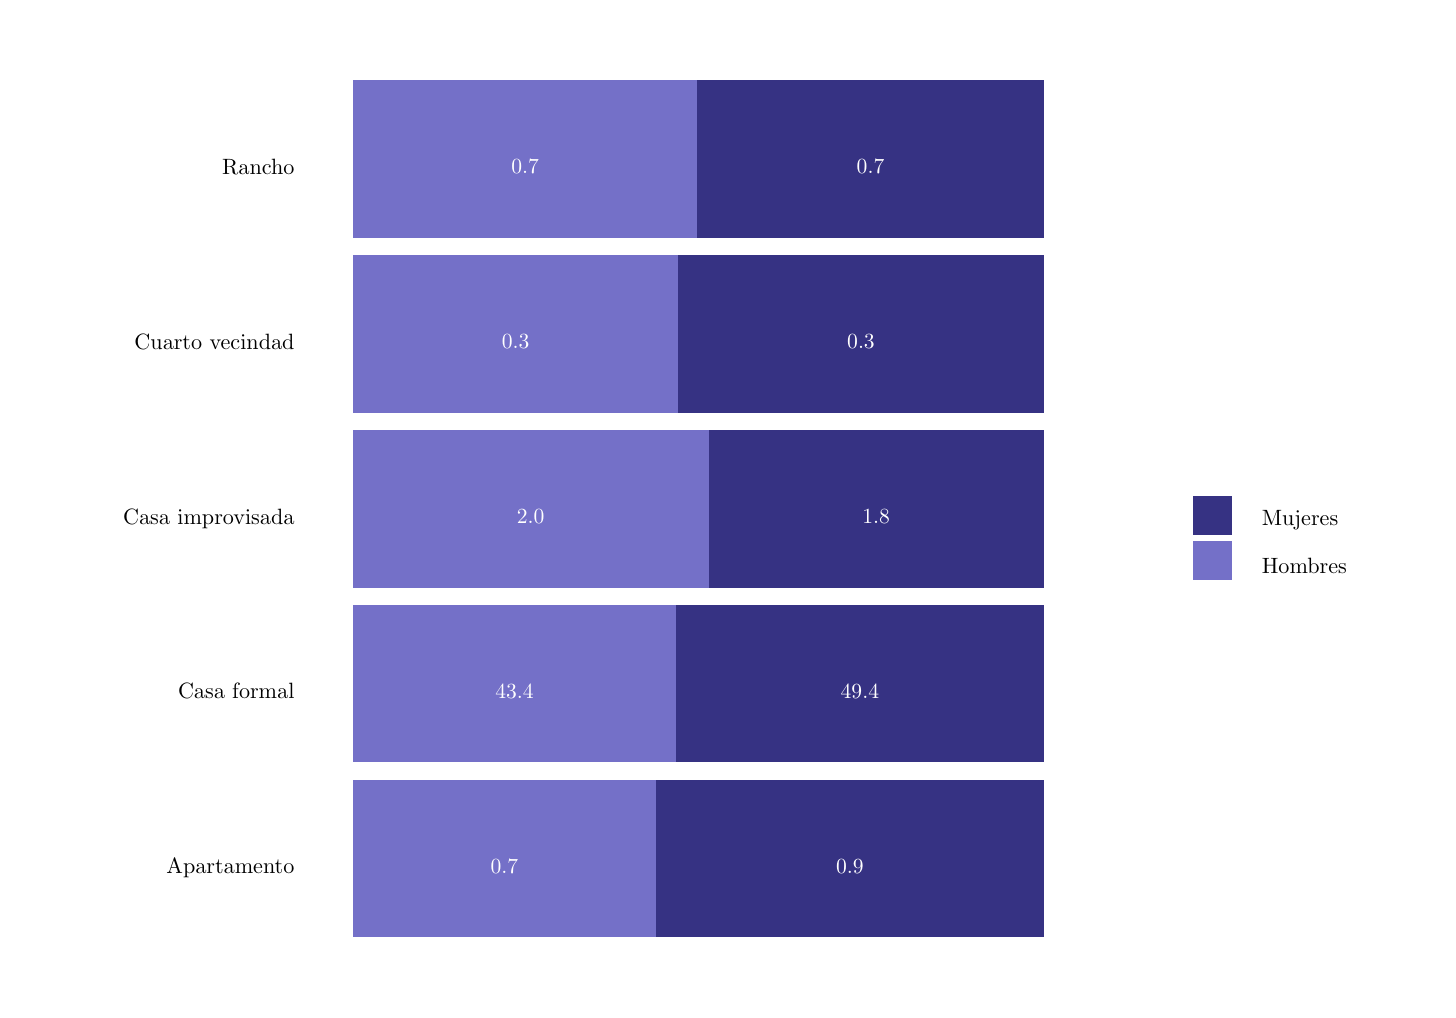
\begin{tikzpicture}[x=1pt,y=1pt, scale = 1.75]% Created by tikzDevice version 0.12.4 on 2023-04-25 12:07:28
% !TEX encoding = UTF-8 Unicode
\definecolor{fillColor}{RGB}{255,255,255}
\path[use as bounding box,fill=fillColor,fill opacity=0.00] (0,0) rectangle (289.08,198.74);
\begin{scope}
\path[clip] (  0.00,  0.00) rectangle (289.08,198.74);
\definecolor{drawColor}{RGB}{255,255,255}
\definecolor{fillColor}{RGB}{255,255,255}

\path[draw=drawColor,line width= 0.6pt,line join=round,line cap=round,fill=fillColor] (  0.00,  0.00) rectangle (289.08,198.74);
\end{scope}
\begin{scope}
\path[clip] (  0.00,  0.00) rectangle (289.08,198.74);
\definecolor{fillColor}{RGB}{54,50,131}

\path[fill=fillColor] (133.87, 47.02) rectangle (209.81, 79.51);

\path[fill=fillColor] (129.74, 10.92) rectangle (209.81, 43.41);

\path[fill=fillColor] (134.34,119.23) rectangle (209.81,151.72);

\path[fill=fillColor] (138.27,155.33) rectangle (209.81,187.83);

\path[fill=fillColor] (140.58, 83.12) rectangle (209.81,115.62);
\definecolor{fillColor}{RGB}{116,112,200}

\path[fill=fillColor] ( 67.17, 47.02) rectangle (133.87, 79.51);

\path[fill=fillColor] ( 67.17, 10.92) rectangle (129.74, 43.41);

\path[fill=fillColor] ( 67.17,119.23) rectangle (134.34,151.72);

\path[fill=fillColor] ( 67.17,155.33) rectangle (138.27,187.83);

\path[fill=fillColor] ( 67.17, 83.12) rectangle (140.58,115.62);
\definecolor{drawColor}{RGB}{255,255,255}

\node[text=drawColor,anchor=base,inner sep=0pt, outer sep=0pt, scale=  0.78] at (171.84, 60.23) {49.4};

\node[text=drawColor,anchor=base,inner sep=0pt, outer sep=0pt, scale=  0.78] at (169.77, 24.13) {0.9};

\node[text=drawColor,anchor=base,inner sep=0pt, outer sep=0pt, scale=  0.78] at (172.07,132.44) {0.3};

\node[text=drawColor,anchor=base,inner sep=0pt, outer sep=0pt, scale=  0.78] at (174.04,168.55) {0.7};

\node[text=drawColor,anchor=base,inner sep=0pt, outer sep=0pt, scale=  0.78] at (175.19, 96.34) {1.8};

\node[text=drawColor,anchor=base,inner sep=0pt, outer sep=0pt, scale=  0.78] at (100.52, 60.23) {43.4};

\node[text=drawColor,anchor=base,inner sep=0pt, outer sep=0pt, scale=  0.78] at ( 98.45, 24.13) {0.7};

\node[text=drawColor,anchor=base,inner sep=0pt, outer sep=0pt, scale=  0.78] at (100.75,132.44) {0.3};

\node[text=drawColor,anchor=base,inner sep=0pt, outer sep=0pt, scale=  0.78] at (102.72,168.55) {0.7};

\node[text=drawColor,anchor=base,inner sep=0pt, outer sep=0pt, scale=  0.78] at (103.87, 96.34) {2.0};
\end{scope}
\begin{scope}
\path[clip] (  0.00,  0.00) rectangle (289.08,198.74);
\definecolor{drawColor}{RGB}{0,0,0}

\node[text=drawColor,anchor=base east,inner sep=0pt, outer sep=0pt, scale=  0.80] at ( 55.08, 24.04) {Apartamento};

\node[text=drawColor,anchor=base east,inner sep=0pt, outer sep=0pt, scale=  0.80] at ( 55.08, 60.14) {Casa formal};

\node[text=drawColor,anchor=base east,inner sep=0pt, outer sep=0pt, scale=  0.80] at ( 55.08, 96.24) {Casa improvisada};

\node[text=drawColor,anchor=base east,inner sep=0pt, outer sep=0pt, scale=  0.80] at ( 55.08,132.35) {Cuarto vecindad};

\node[text=drawColor,anchor=base east,inner sep=0pt, outer sep=0pt, scale=  0.80] at ( 55.08,168.45) {Rancho};
\end{scope}
\begin{scope}
\path[clip] (  0.00,  0.00) rectangle (289.08,198.74);
\definecolor{fillColor}{RGB}{255,255,255}

\path[fill=fillColor] (227.94, 70.00) rectangle (283.58,128.74);
\end{scope}
\begin{scope}
\path[clip] (  0.00,  0.00) rectangle (289.08,198.74);
\definecolor{drawColor}{RGB}{0,0,0}

\node[text=drawColor,anchor=base west,inner sep=0pt, outer sep=0pt, scale=  1.00] at (233.44,114.11) { };
\end{scope}
\begin{scope}
\path[clip] (  0.00,  0.00) rectangle (289.08,198.74);
\definecolor{fillColor}{gray}{0.95}

%\path[fill=fillColor] (237.96, 91.40) rectangle (249.34,102.78);
\end{scope}
\begin{scope}
\path[clip] (  0.00,  0.00) rectangle (289.08,198.74);
\definecolor{fillColor}{RGB}{54,50,131}

\path[fill=fillColor] (240.62, 94.06) rectangle (248.67,102.12);
\end{scope}
\begin{scope}
\path[clip] (  0.00,  0.00) rectangle (289.08,198.74);
\definecolor{fillColor}{gray}{0.95}

%\path[fill=fillColor] (237.96, 80.02) rectangle (249.34, 91.40);
\end{scope}
\begin{scope}
\path[clip] (  0.00,  0.00) rectangle (289.08,198.74);
\definecolor{fillColor}{RGB}{116,112,200}

\path[fill=fillColor] (240.62, 84.68) rectangle (248.67, 92.74);
\end{scope}
\begin{scope}
\path[clip] (  0.00,  0.00) rectangle (289.08,198.74);
\definecolor{drawColor}{RGB}{0,0,0}

\node[text=drawColor,anchor=base west,inner sep=0pt, outer sep=0pt, scale=  0.80] at (254.84, 95.96) {Mujeres};
\end{scope}
\begin{scope}
\path[clip] (  0.00,  0.00) rectangle (289.08,198.74);
\definecolor{drawColor}{RGB}{0,0,0}

\node[text=drawColor,anchor=base west,inner sep=0pt, outer sep=0pt, scale=  0.80] at (254.84, 85.98) {Hombres};
\end{scope}\end{tikzpicture}}{INE - ENEI 2022}

\cajota{Mapa departamental por número de mujeres}{Para 2023, según estimaciones del Instituto Nacional de Estadística basadas en el Censo 2018, el departamento con mayor población de mujeres es el departamento de Guatemala con 1,884,252 mujeres, seguido de Huehuetenando con 736,230 mujeres. Los departamentos con menor proyección poblacional de mujeres son El Progreso con 99,546 mujeres y Zacapa con 140,863 mujeres. }{Proyección de población de mujeres por departamento (número de mujeres)}{República de Guatemala, Instituto Nacional de Estadística}{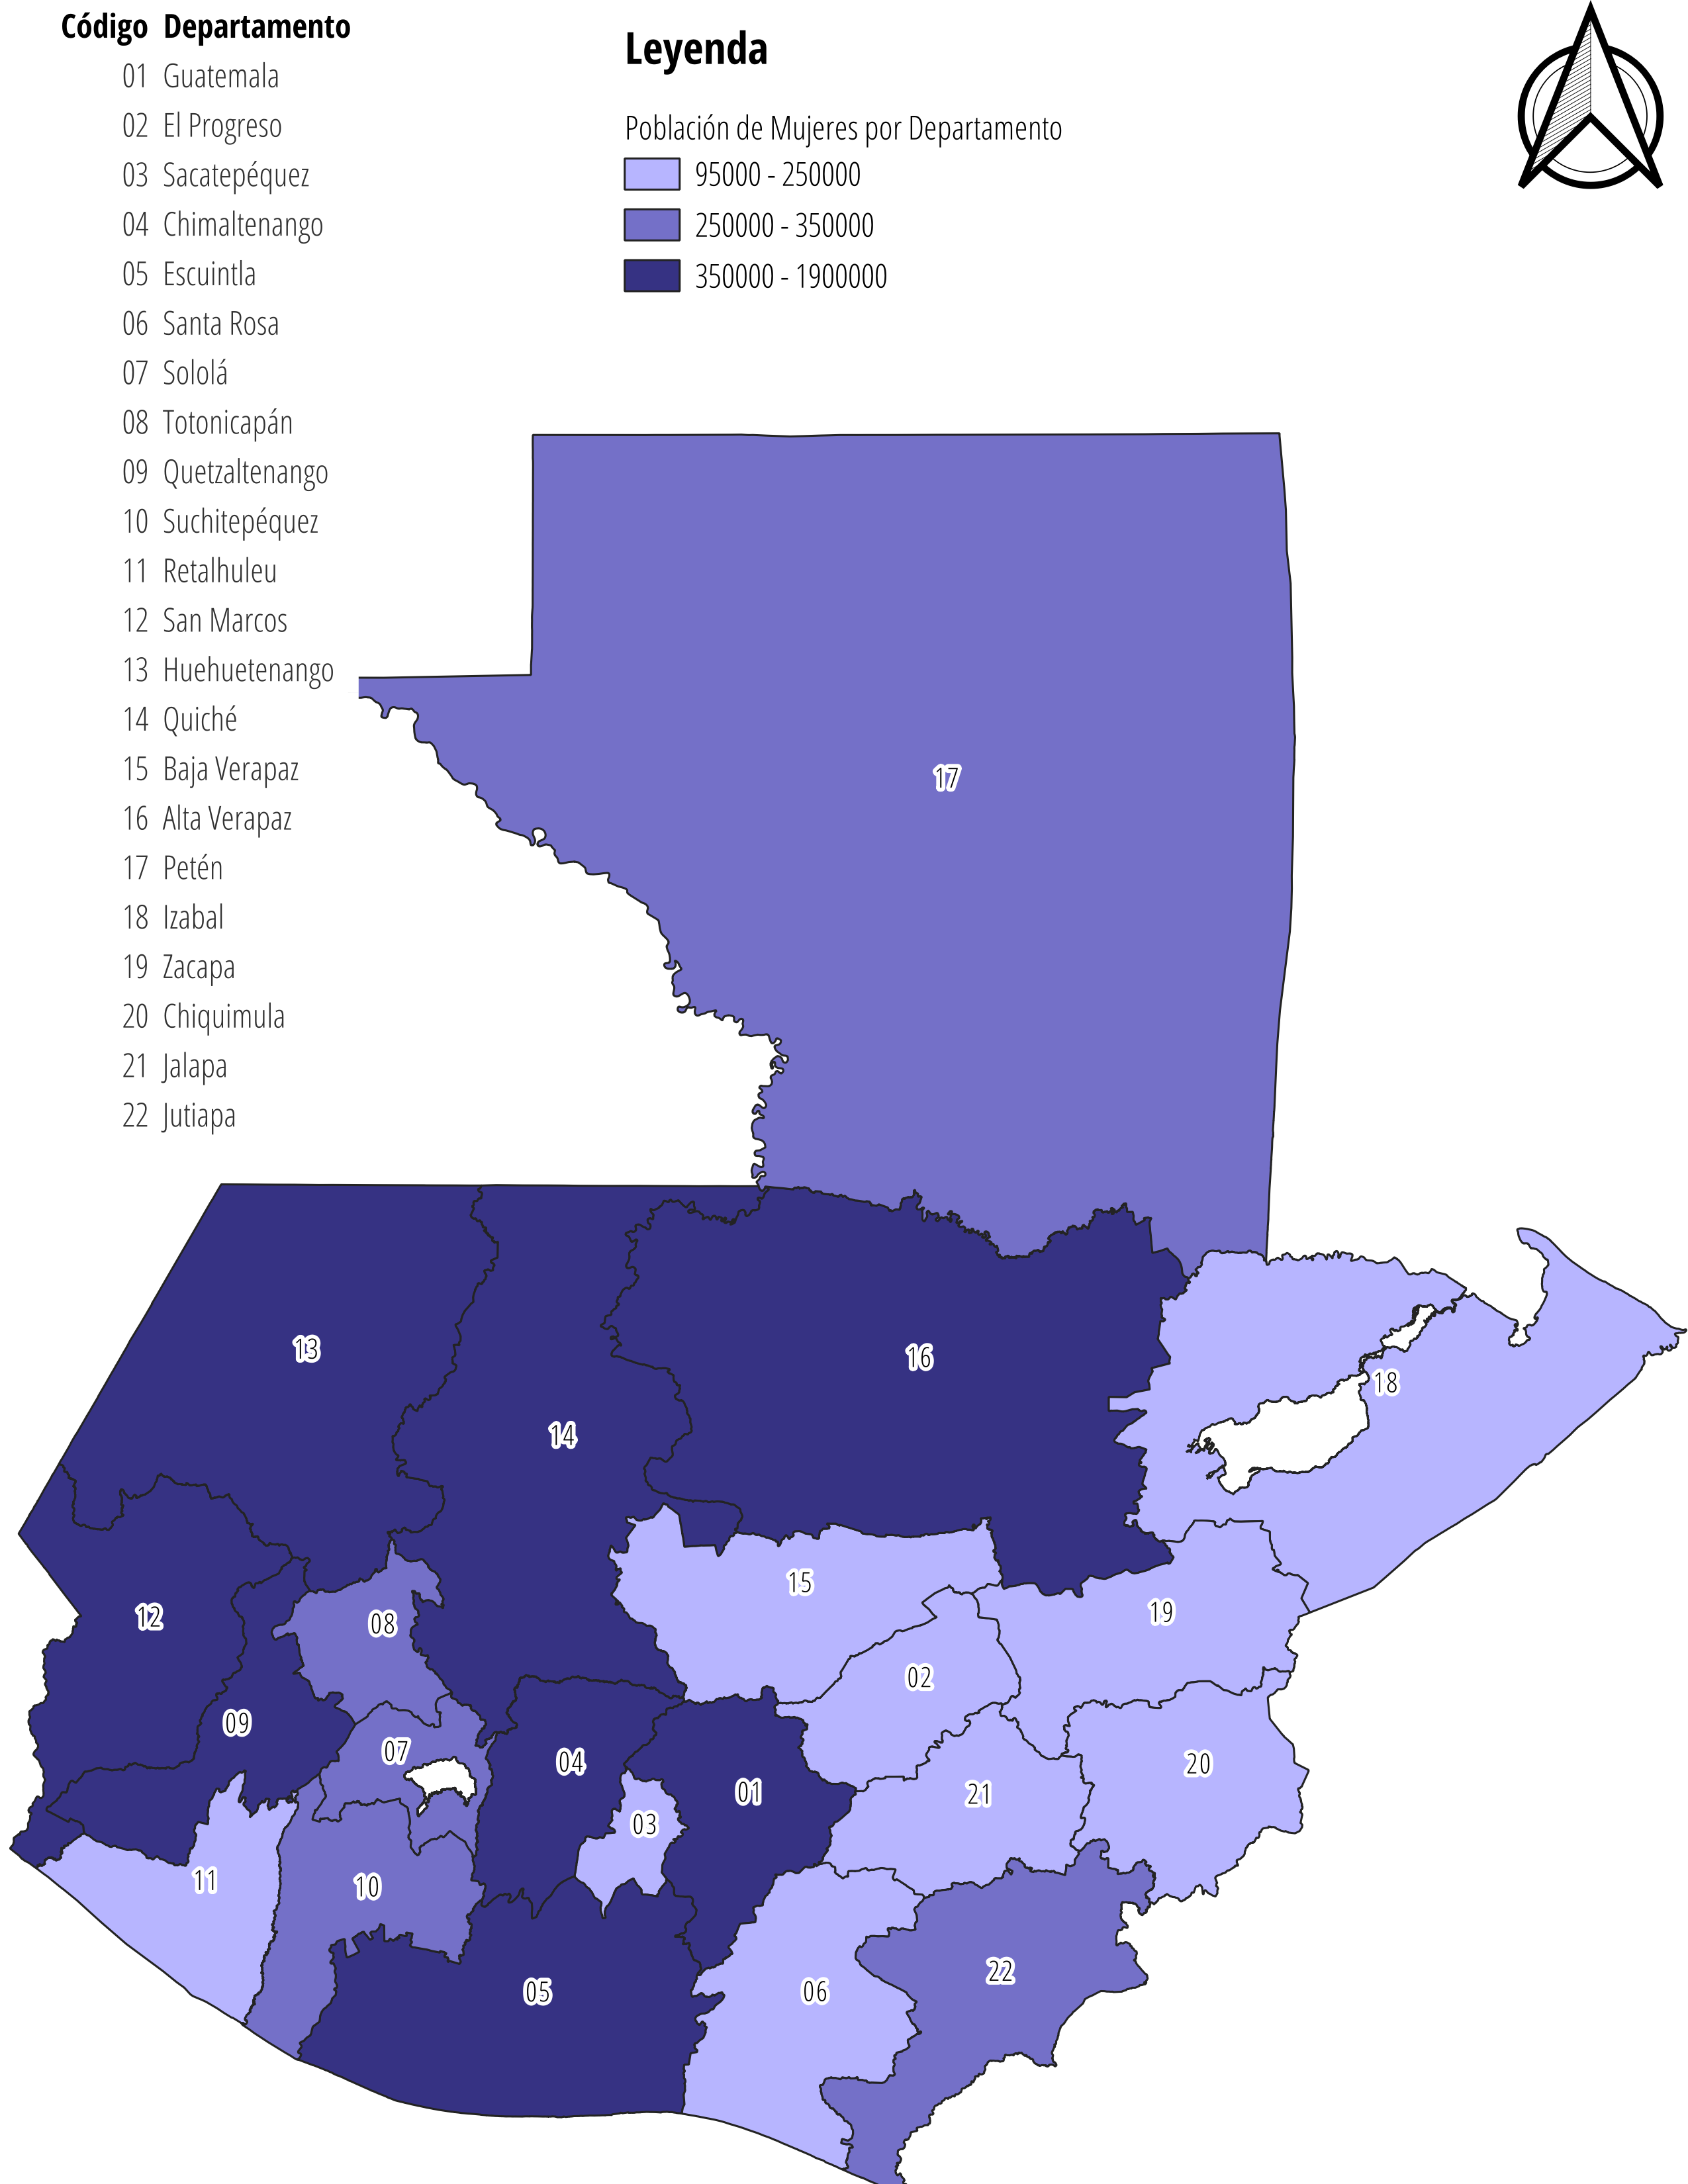
\includegraphics[width=0.75\textwidth]{Graficas/mapa_departamental}}{INE - Proyecciones 2020}

\cajota{Mapa municipal por número de mujeres}{\justifying Para 2022, según estimaciones del Instituto Nacional de Estadística, el municipio con mayor población fue Guatemala con 630,634 mujeres, seguido de Mixco con 269,358 mujeres. Los municipios con menor proyección poblacional de mujeres fueron Santa María Visitación con 1,354 mujeres y San Marcos La Laguna con 1,531 mujeres.  }{Proyección de población de mujeres por municipio (número de mujeres)}{República de Guatemala, Instituto Nacional de Estadística}{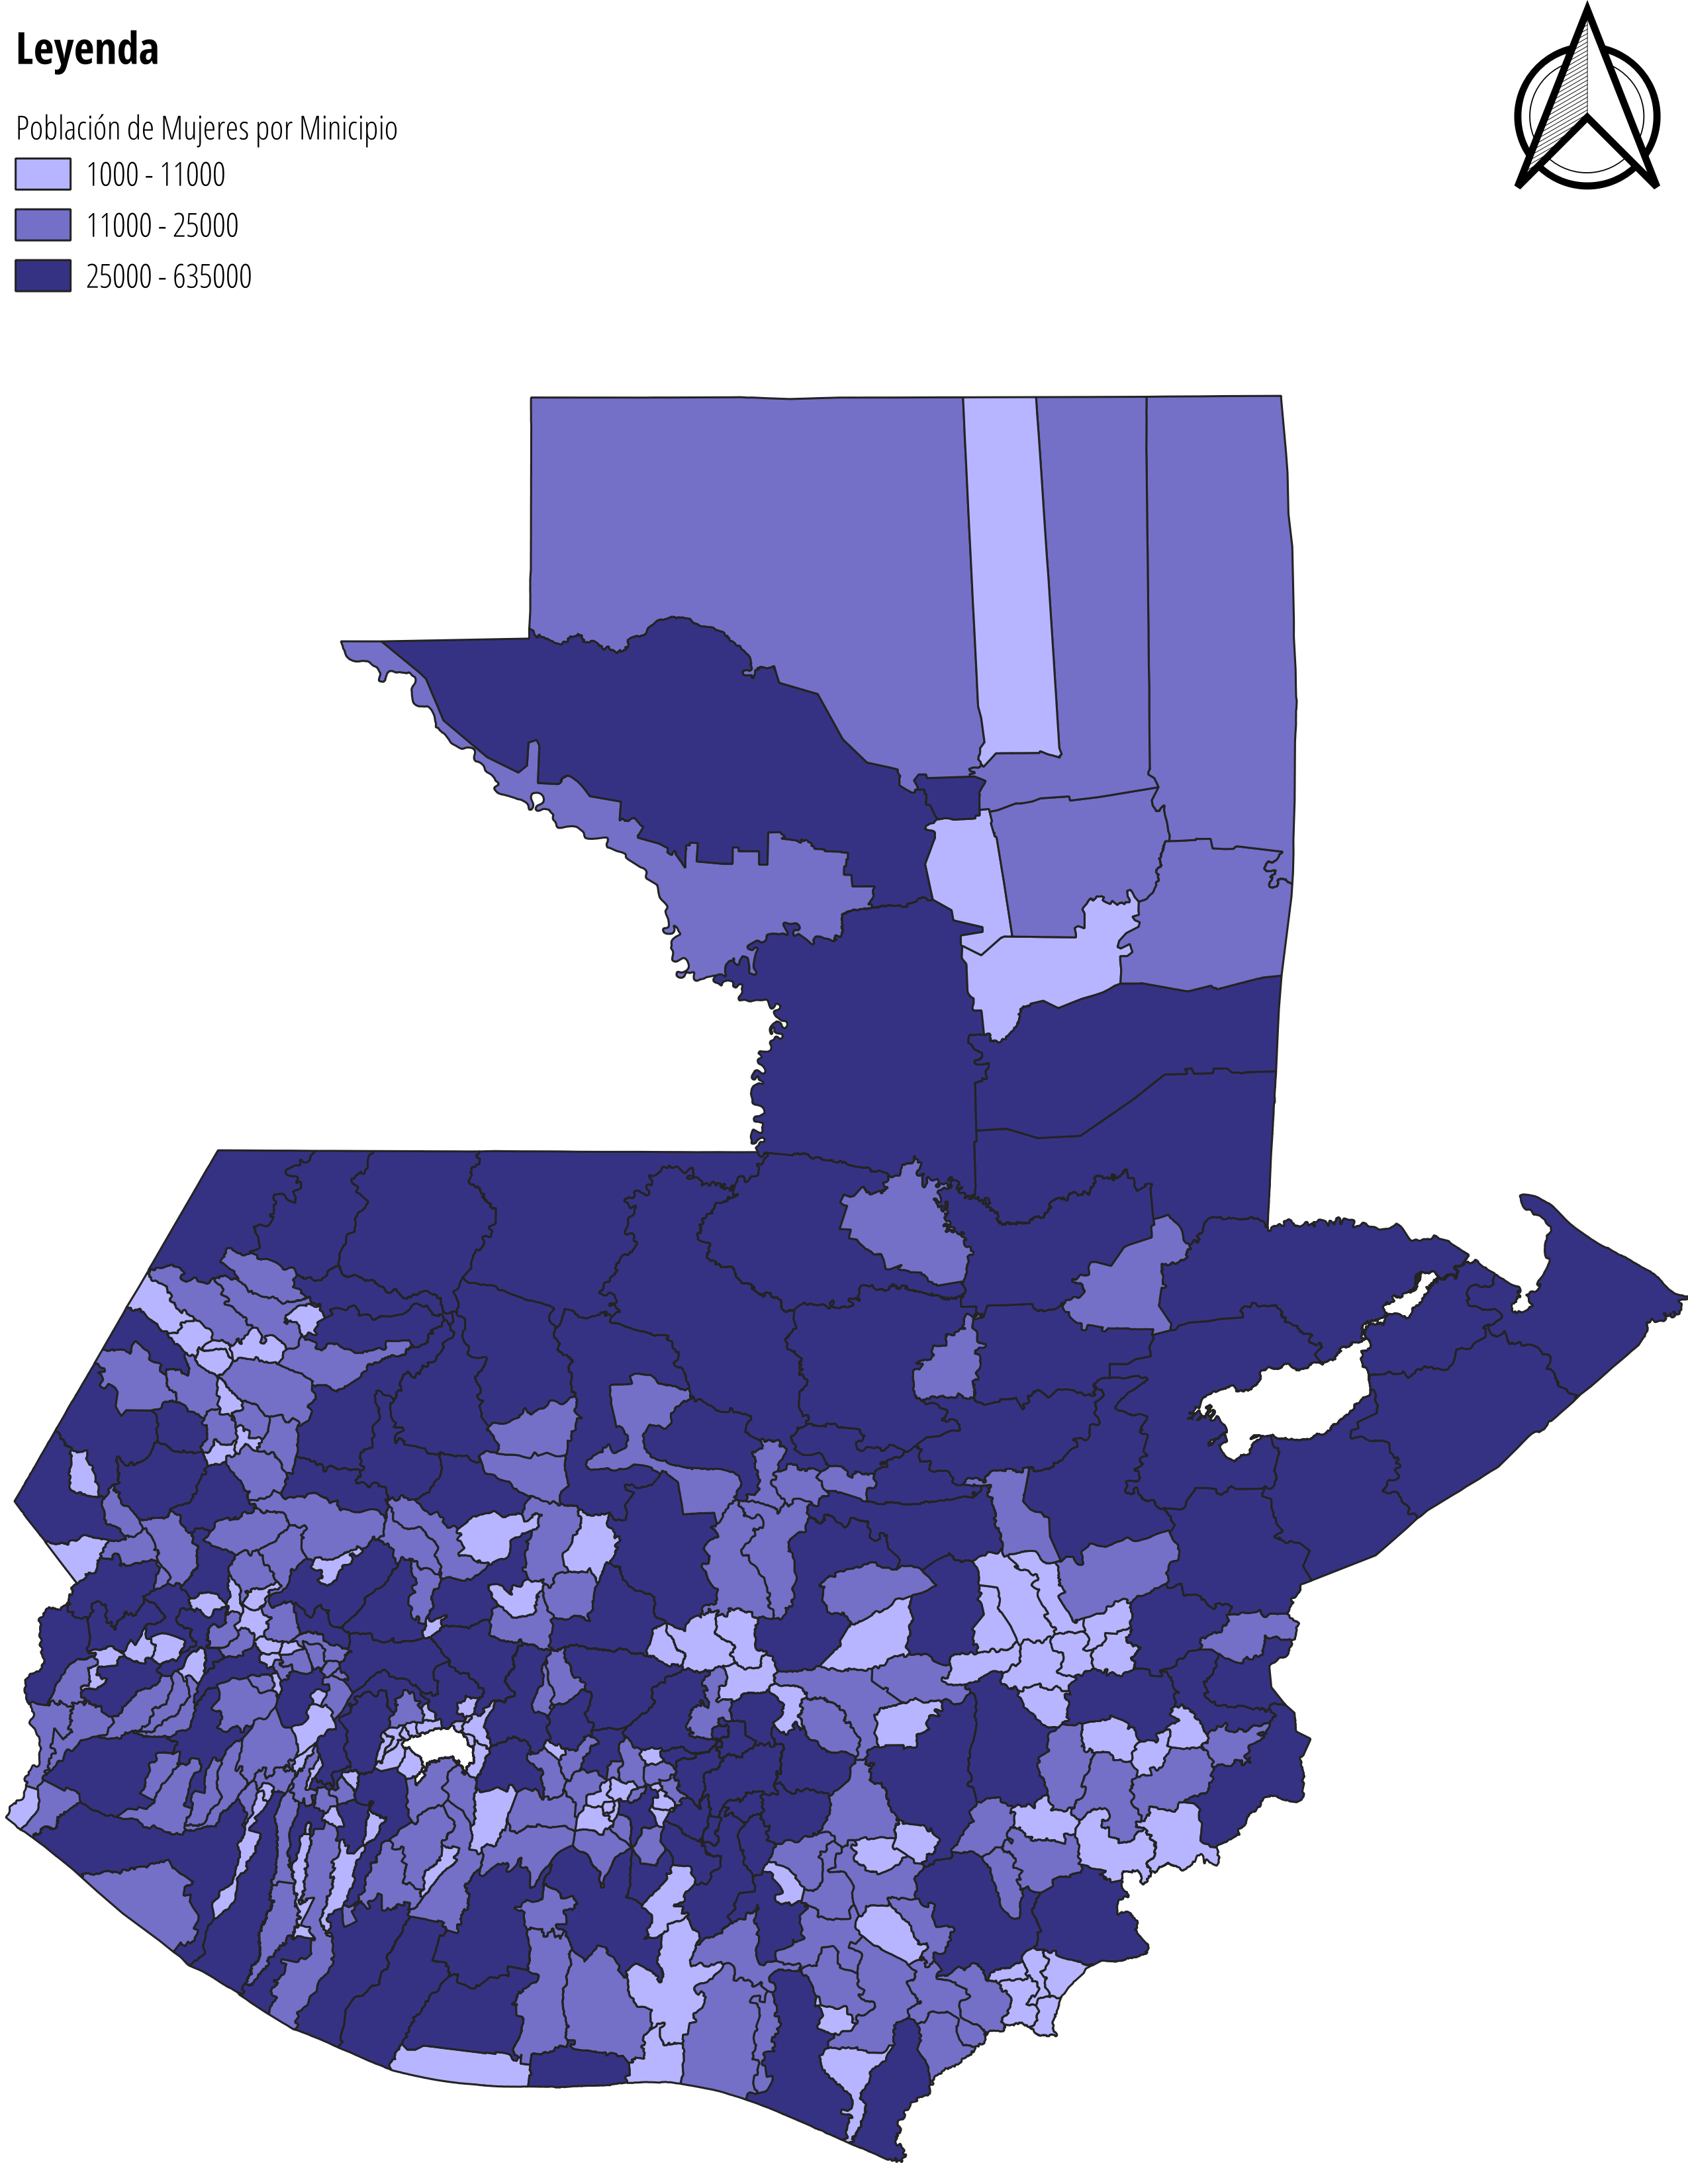
\includegraphics[width=0.75\textwidth]{Graficas/mapa_municipal}}{INE - Proyecciones 2020}

\cajita{Esperanza de vida al nacer por sexo}{La esperanza de vida al nacer indica la cantidad de años que se espera que viva la persona nacida en un periodo de tiempo determinado. En Guatemala, las mujeres tienen una esperanza de vida mayor que los hombres. El período de referencia es tomado hasta el 30 junio de cada año. }{Serie histórica de esperanza de vida (número de años)}{República de Guatemala, Instituto Nacional de Estadística}{\begin{tikzpicture}[x=1pt,y=1pt]% Created by tikzDevice version 0.12.4 on 2023-05-15 10:48:14
% !TEX encoding = UTF-8 Unicode
\definecolor{fillColor}{RGB}{255,255,255}
\path[use as bounding box,fill=fillColor,fill opacity=0.00] (0,0) rectangle (289.08,198.74);
\begin{scope}
\path[clip] (  0.00,  0.00) rectangle (289.08,198.74);

\path[] (  0.00,  0.00) rectangle (289.08,198.74);
\end{scope}
\begin{scope}
\path[clip] (  0.00,  0.00) rectangle (289.08,198.74);
\definecolor{drawColor}{RGB}{54,50,131}

\path[draw=drawColor,line width= 1.7pt,line join=round] ( 31.91,128.88) --
	( 85.96,130.22) --
	(140.01,131.55) --
	(194.06,132.89) --
	(248.11,134.22);
\definecolor{drawColor}{RGB}{116,112,200}

\path[draw=drawColor,line width= 1.7pt,line join=round] ( 31.91, 85.49) --
	( 85.96, 86.82) --
	(140.01, 88.16) --
	(194.06, 89.49) --
	(248.11, 90.83);
\definecolor{drawColor}{RGB}{0,0,0}

\node[text=drawColor,anchor=base,inner sep=0pt, outer sep=0pt, scale=  1.02] at ( 31.91,116.97) {75.8};

\node[text=drawColor,anchor=base east,inner sep=0pt, outer sep=0pt, scale=  1.02] at ( 82.83,130.22) {76.0};

\node[text=drawColor,anchor=base east,inner sep=0pt, outer sep=0pt, scale=  1.02] at (136.88,131.55) {76.2};

\node[text=drawColor,anchor=base east,inner sep=0pt, outer sep=0pt, scale=  1.02] at (190.94,132.89) {76.4};

\node[text=drawColor,anchor=base,inner sep=0pt, outer sep=0pt, scale=  1.02] at (248.11,138.19) {76.6};

\node[text=drawColor,anchor=base,inner sep=0pt, outer sep=0pt, scale=  1.02] at ( 31.91, 73.58) {69.3};

\node[text=drawColor,anchor=base east,inner sep=0pt, outer sep=0pt, scale=  1.02] at ( 82.83, 86.82) {69.5};

\node[text=drawColor,anchor=base east,inner sep=0pt, outer sep=0pt, scale=  1.02] at (136.88, 88.16) {69.7};

\node[text=drawColor,anchor=base east,inner sep=0pt, outer sep=0pt, scale=  1.02] at (190.94, 89.49) {69.9};

\node[text=drawColor,anchor=base,inner sep=0pt, outer sep=0pt, scale=  1.02] at (248.11, 94.80) {70.1};

\path[draw=drawColor,line width= 0.1pt,line join=round] (-281.58, 23.41) -- (561.61, 23.41);

\path[] ( -0.52, 15.40) rectangle (280.54,191.63);

\path[] ( -0.52, 40.10) --
	(280.54, 40.10);

\path[] ( -0.52, 73.47) --
	(280.54, 73.47);

\path[] ( -0.52,106.85) --
	(280.54,106.85);

\path[] ( -0.52,140.23) --
	(280.54,140.23);

\path[] ( -0.52,173.61) --
	(280.54,173.61);

\path[] ( -0.52, 23.41) --
	(280.54, 23.41);

\path[] ( -0.52, 56.79) --
	(280.54, 56.79);

\path[] ( -0.52, 90.16) --
	(280.54, 90.16);

\path[] ( -0.52,123.54) --
	(280.54,123.54);

\path[] ( -0.52,156.92) --
	(280.54,156.92);

\path[] ( -0.52,190.29) --
	(280.54,190.29);

\path[] ( 31.91, 15.40) --
	( 31.91,191.63);

\path[] ( 85.96, 15.40) --
	( 85.96,191.63);

\path[] (140.01, 15.40) --
	(140.01,191.63);

\path[] (194.06, 15.40) --
	(194.06,191.63);

\path[] (248.11, 15.40) --
	(248.11,191.63);

\path[] ( -0.52, 15.40) rectangle (280.54,191.63);
\end{scope}
\begin{scope}
\path[clip] (  0.00,  0.00) rectangle (289.08,198.74);

\path[] ( -0.52, 15.40) --
	( -0.52,191.63);
\end{scope}
\begin{scope}
\path[clip] (  0.00,  0.00) rectangle (289.08,198.74);
\definecolor{drawColor}{RGB}{255,255,255}

\node[text=drawColor,text opacity=0.00,anchor=base east,inner sep=0pt, outer sep=0pt, scale=  1.00] at ( -5.47, 19.50) {60};

\node[text=drawColor,text opacity=0.00,anchor=base east,inner sep=0pt, outer sep=0pt, scale=  1.00] at ( -5.47, 52.88) {65};

\node[text=drawColor,text opacity=0.00,anchor=base east,inner sep=0pt, outer sep=0pt, scale=  1.00] at ( -5.47, 86.25) {70};

\node[text=drawColor,text opacity=0.00,anchor=base east,inner sep=0pt, outer sep=0pt, scale=  1.00] at ( -5.47,119.63) {75};

\node[text=drawColor,text opacity=0.00,anchor=base east,inner sep=0pt, outer sep=0pt, scale=  1.00] at ( -5.47,153.01) {80};

\node[text=drawColor,text opacity=0.00,anchor=base east,inner sep=0pt, outer sep=0pt, scale=  1.00] at ( -5.47,186.39) {85};
\end{scope}
\begin{scope}
\path[clip] (  0.00,  0.00) rectangle (289.08,198.74);

\path[] ( -3.27, 23.41) --
	( -0.52, 23.41);

\path[] ( -3.27, 56.79) --
	( -0.52, 56.79);

\path[] ( -3.27, 90.16) --
	( -0.52, 90.16);

\path[] ( -3.27,123.54) --
	( -0.52,123.54);

\path[] ( -3.27,156.92) --
	( -0.52,156.92);

\path[] ( -3.27,190.29) --
	( -0.52,190.29);
\end{scope}
\begin{scope}
\path[clip] (  0.00,  0.00) rectangle (289.08,198.74);

\path[] ( -0.52, 15.40) --
	(280.54, 15.40);
\end{scope}
\begin{scope}
\path[clip] (  0.00,  0.00) rectangle (289.08,198.74);

\path[] ( 31.91, 12.65) --
	( 31.91, 15.40);

\path[] ( 85.96, 12.65) --
	( 85.96, 15.40);

\path[] (140.01, 12.65) --
	(140.01, 15.40);

\path[] (194.06, 12.65) --
	(194.06, 15.40);

\path[] (248.11, 12.65) --
	(248.11, 15.40);
\end{scope}
\begin{scope}
\path[clip] (  0.00,  0.00) rectangle (289.08,198.74);
\definecolor{drawColor}{RGB}{0,0,0}

\node[text=drawColor,anchor=base,inner sep=0pt, outer sep=0pt, scale=  1.00] at ( 31.91,  1.32) {2017-2018};

\node[text=drawColor,anchor=base,inner sep=0pt, outer sep=0pt, scale=  1.00] at ( 85.96,  1.32) {2018-2019};

\node[text=drawColor,anchor=base,inner sep=0pt, outer sep=0pt, scale=  1.00] at (140.01,  1.32) {2019-2020};

\node[text=drawColor,anchor=base,inner sep=0pt, outer sep=0pt, scale=  1.00] at (194.06,  1.32) {2020-2021};

\node[text=drawColor,anchor=base,inner sep=0pt, outer sep=0pt, scale=  1.00] at (248.11,  1.32) {2021-2022};
\end{scope}
\begin{scope}
\path[clip] (  0.00,  0.00) rectangle (289.08,198.74);
\coordinate (apoyo) at (54.45,189.21);
\coordinate (longitudFicticia) at (7.11,9.53);
\coordinate (longitud) at (7.11,7.11);
\coordinate (desX) at (137.12,0);
\coordinate (desY) at (0,1.21);
\definecolor[named]{ct1}{HTML}{
363283
}
\definecolor[named]{ct2}{HTML}{
7470C8
}
\definecolor[named]{ctb1}{HTML}{
363283
}
\definecolor[named]{ctb2}{HTML}{
7470C8
}
\path [fill=none] (apoyo) rectangle ($(apoyo)+(longitudFicticia)$)
node [xshift=0.3cm,inner sep=0pt, outer sep=0pt,midway,right,scale = 1]{Mujeres};
\draw [color = ctb1,fill=ct1] ( $(apoyo)  + (desY) $) rectangle ($(apoyo)+ (desY) +(longitud)$);
\path [fill=none] ($(apoyo)+(desX)$) rectangle ($(apoyo)+(desX)+(longitudFicticia)$)
node [xshift=0.3cm,inner sep=0pt, outer sep=0pt,midway,right,scale = 1]{Hombres};
\draw [color = ctb2 ,fill=ct2] ( $(apoyo)  + (desY) + (desX) $) rectangle ($(apoyo)+ (desY)+ (desX) +(longitud)$);
\end{scope}
\end{tikzpicture}}{INE y CELADE - 2019}{}

\cajita{Tasa global de fecundidad (mujeres 15 a 49 años)}{El valor de la Tasa Global de Fecundidad (TGF) se interpreta como el número de hijos e hijas, que en promedio tendría una mujer de una cohorte hipotética de mujeres no expuestas al riesgo de muerte desde el inicio hasta el fin del periodo fértil y que, a partir del momento en que se inicia la reproducción están expuestas a las tasas de fecundidad por edad de la población en estudio. 

En Guatemala tanto en 2020 como en 2021 se reportó la misma tasa de 2.3 hijas(os) por mujer.}{Serie histórica de tasa global de fecundidad (número de hijas(os))}{República de Guatemala, Instituto Nacional de Estadística}{\begin{tikzpicture}[x=1pt,y=1pt]% Created by tikzDevice version 0.12.4 on 2023-04-24 14:16:45
% !TEX encoding = UTF-8 Unicode
\definecolor{fillColor}{RGB}{255,255,255}
\path[use as bounding box,fill=fillColor,fill opacity=0.00] (0,0) rectangle (289.08,198.74);
\begin{scope}
\path[clip] (  0.00,  0.00) rectangle (289.08,198.74);

\path[] (  0.00,  0.00) rectangle (289.08,198.74);
\end{scope}
\begin{scope}
\path[clip] (  0.00,  0.00) rectangle (289.08,198.74);
\definecolor{drawColor}{RGB}{54,50,131}

\path[draw=drawColor,line width= 1.7pt,line join=round] ( 48.88,181.44) --
	(113.23,131.32) --
	(177.58, 63.72) --
	(241.93, 61.88);
\definecolor{drawColor}{RGB}{0,0,0}

\node[text=drawColor,anchor=base,inner sep=0pt, outer sep=0pt, scale=  1.02] at ( 48.88,185.41) {2.6};

\node[text=drawColor,anchor=base west,inner sep=0pt, outer sep=0pt, scale=  1.02] at (113.23,135.29) {2.5};

\node[text=drawColor,anchor=base west,inner sep=0pt, outer sep=0pt, scale=  1.02] at (177.58, 67.69) {2.3};

\node[text=drawColor,anchor=base,inner sep=0pt, outer sep=0pt, scale=  1.02] at (241.93, 49.97) {2.3};

\path[draw=drawColor,line width= 0.1pt,line join=round] (-260.00, 26.01) -- (550.81, 26.01);

\path[] ( 10.27, 18.24) rectangle (280.54,189.21);

\path[] ( 10.27, 26.47) --
	(280.54, 26.47);

\path[] ( 10.27, 58.93) --
	(280.54, 58.93);

\path[] ( 10.27, 91.39) --
	(280.54, 91.39);

\path[] ( 10.27,123.84) --
	(280.54,123.84);

\path[] ( 10.27,156.30) --
	(280.54,156.30);

\path[] ( 10.27,188.76) --
	(280.54,188.76);

\path[] ( 10.27, 42.70) --
	(280.54, 42.70);

\path[] ( 10.27, 75.16) --
	(280.54, 75.16);

\path[] ( 10.27,107.61) --
	(280.54,107.61);

\path[] ( 10.27,140.07) --
	(280.54,140.07);

\path[] ( 10.27,172.53) --
	(280.54,172.53);

\path[] ( 48.88, 18.24) --
	( 48.88,189.21);

\path[] (113.23, 18.24) --
	(113.23,189.21);

\path[] (177.58, 18.24) --
	(177.58,189.21);

\path[] (241.93, 18.24) --
	(241.93,189.21);

\path[] ( 10.27, 18.24) rectangle (280.54,189.21);
\end{scope}
\begin{scope}
\path[clip] (  0.00,  0.00) rectangle (289.08,198.74);

\path[] ( 10.27, 18.24) --
	( 10.27,189.21);
\end{scope}
\begin{scope}
\path[clip] (  0.00,  0.00) rectangle (289.08,198.74);
\definecolor{drawColor}{RGB}{255,255,255}

\node[text=drawColor,text opacity=0.00,anchor=base east,inner sep=0pt, outer sep=0pt, scale=  1.00] at (  5.32, 38.79) {2.2};

\node[text=drawColor,text opacity=0.00,anchor=base east,inner sep=0pt, outer sep=0pt, scale=  1.00] at (  5.32, 71.25) {2.3};

\node[text=drawColor,text opacity=0.00,anchor=base east,inner sep=0pt, outer sep=0pt, scale=  1.00] at (  5.32,103.71) {2.4};

\node[text=drawColor,text opacity=0.00,anchor=base east,inner sep=0pt, outer sep=0pt, scale=  1.00] at (  5.32,136.16) {2.5};

\node[text=drawColor,text opacity=0.00,anchor=base east,inner sep=0pt, outer sep=0pt, scale=  1.00] at (  5.32,168.62) {2.6};
\end{scope}
\begin{scope}
\path[clip] (  0.00,  0.00) rectangle (289.08,198.74);

\path[] (  7.52, 42.70) --
	( 10.27, 42.70);

\path[] (  7.52, 75.16) --
	( 10.27, 75.16);

\path[] (  7.52,107.61) --
	( 10.27,107.61);

\path[] (  7.52,140.07) --
	( 10.27,140.07);

\path[] (  7.52,172.53) --
	( 10.27,172.53);
\end{scope}
\begin{scope}
\path[clip] (  0.00,  0.00) rectangle (289.08,198.74);

\path[] ( 10.27, 18.24) --
	(280.54, 18.24);
\end{scope}
\begin{scope}
\path[clip] (  0.00,  0.00) rectangle (289.08,198.74);

\path[] ( 48.88, 15.49) --
	( 48.88, 18.24);

\path[] (113.23, 15.49) --
	(113.23, 18.24);

\path[] (177.58, 15.49) --
	(177.58, 18.24);

\path[] (241.93, 15.49) --
	(241.93, 18.24);
\end{scope}
\begin{scope}
\path[clip] (  0.00,  0.00) rectangle (289.08,198.74);
\definecolor{drawColor}{RGB}{0,0,0}

\node[text=drawColor,anchor=base,inner sep=0pt, outer sep=0pt, scale=  1.00] at ( 48.88,  4.16) {2018};

\node[text=drawColor,anchor=base,inner sep=0pt, outer sep=0pt, scale=  1.00] at (113.23,  4.16) {2019};

\node[text=drawColor,anchor=base,inner sep=0pt, outer sep=0pt, scale=  1.00] at (177.58,  4.16) {2020};

\node[text=drawColor,anchor=base,inner sep=0pt, outer sep=0pt, scale=  1.00] at (241.93,  4.16) {2021};
\end{scope}
\end{tikzpicture}}{INE - Estadísticas Vitales}{}

\cajita{Tasa de fecundidad juvenil según edades simples (13-19 años)}{La tasa específica de fecundidad es el número de nacimientos por cada mil mujeres en la edad de 15 a 19. En Guatemala se reportó en 2021 una tasa específica de fecundidad de 51.4 hijas(os) cada mil mujeres.}{Tasa de fecundidad juvenil según edades simples (13-19 años) (número de hijas(os))}{República de Guatemala, Instituto Nacional de Estadística}{\begin{tikzpicture}[x=1pt,y=1pt]% Created by tikzDevice version 0.12.4 on 2023-04-24 14:16:56
% !TEX encoding = UTF-8 Unicode
\definecolor{fillColor}{RGB}{255,255,255}
\path[use as bounding box,fill=fillColor,fill opacity=0.00] (0,0) rectangle (289.08,198.74);
\begin{scope}
\path[clip] (  0.00,  0.00) rectangle (289.08,198.74);

\path[] (  0.00,  0.00) rectangle (289.08,198.74);
\end{scope}
\begin{scope}
\path[clip] (  0.00,  0.00) rectangle (289.08,198.74);
\definecolor{drawColor}{RGB}{54,50,131}

\path[draw=drawColor,line width= 1.7pt,line join=round] ( 39.63,181.44) --
	(106.55,136.50) --
	(173.47, 61.88) --
	(240.39, 72.67);
\definecolor{drawColor}{RGB}{0,0,0}

\node[text=drawColor,anchor=base,inner sep=0pt, outer sep=0pt, scale=  1.02] at ( 39.63,185.41) {60.1};

\node[text=drawColor,anchor=base west,inner sep=0pt, outer sep=0pt, scale=  1.02] at (106.55,140.47) {56.5};

\node[text=drawColor,anchor=base,inner sep=0pt, outer sep=0pt, scale=  1.02] at (173.47, 49.97) {50.5};

\node[text=drawColor,anchor=base,inner sep=0pt, outer sep=0pt, scale=  1.02] at (240.39, 76.64) {51.4};

\path[draw=drawColor,line width= 0.1pt,line join=round] (-281.58, 26.01) -- (561.61, 26.01);

\path[] ( -0.52, 18.24) rectangle (280.54,189.21);

\path[] ( -0.52, 55.11) --
	(280.54, 55.11);

\path[] ( -0.52,104.99) --
	(280.54,104.99);

\path[] ( -0.52,154.87) --
	(280.54,154.87);

\path[] ( -0.52, 30.17) --
	(280.54, 30.17);

\path[] ( -0.52, 80.05) --
	(280.54, 80.05);

\path[] ( -0.52,129.93) --
	(280.54,129.93);

\path[] ( -0.52,179.81) --
	(280.54,179.81);

\path[] ( 39.63, 18.24) --
	( 39.63,189.21);

\path[] (106.55, 18.24) --
	(106.55,189.21);

\path[] (173.47, 18.24) --
	(173.47,189.21);

\path[] (240.39, 18.24) --
	(240.39,189.21);

\path[] ( -0.52, 18.24) rectangle (280.54,189.21);
\end{scope}
\begin{scope}
\path[clip] (  0.00,  0.00) rectangle (289.08,198.74);

\path[] ( -0.52, 18.24) --
	( -0.52,189.21);
\end{scope}
\begin{scope}
\path[clip] (  0.00,  0.00) rectangle (289.08,198.74);
\definecolor{drawColor}{RGB}{255,255,255}

\node[text=drawColor,text opacity=0.00,anchor=base east,inner sep=0pt, outer sep=0pt, scale=  1.00] at ( -5.47, 26.26) {48};

\node[text=drawColor,text opacity=0.00,anchor=base east,inner sep=0pt, outer sep=0pt, scale=  1.00] at ( -5.47, 76.14) {52};

\node[text=drawColor,text opacity=0.00,anchor=base east,inner sep=0pt, outer sep=0pt, scale=  1.00] at ( -5.47,126.02) {56};

\node[text=drawColor,text opacity=0.00,anchor=base east,inner sep=0pt, outer sep=0pt, scale=  1.00] at ( -5.47,175.91) {60};
\end{scope}
\begin{scope}
\path[clip] (  0.00,  0.00) rectangle (289.08,198.74);

\path[] ( -3.27, 30.17) --
	( -0.52, 30.17);

\path[] ( -3.27, 80.05) --
	( -0.52, 80.05);

\path[] ( -3.27,129.93) --
	( -0.52,129.93);

\path[] ( -3.27,179.81) --
	( -0.52,179.81);
\end{scope}
\begin{scope}
\path[clip] (  0.00,  0.00) rectangle (289.08,198.74);

\path[] ( -0.52, 18.24) --
	(280.54, 18.24);
\end{scope}
\begin{scope}
\path[clip] (  0.00,  0.00) rectangle (289.08,198.74);

\path[] ( 39.63, 15.49) --
	( 39.63, 18.24);

\path[] (106.55, 15.49) --
	(106.55, 18.24);

\path[] (173.47, 15.49) --
	(173.47, 18.24);

\path[] (240.39, 15.49) --
	(240.39, 18.24);
\end{scope}
\begin{scope}
\path[clip] (  0.00,  0.00) rectangle (289.08,198.74);
\definecolor{drawColor}{RGB}{0,0,0}

\node[text=drawColor,anchor=base,inner sep=0pt, outer sep=0pt, scale=  1.00] at ( 39.63,  4.16) {2018};

\node[text=drawColor,anchor=base,inner sep=0pt, outer sep=0pt, scale=  1.00] at (106.55,  4.16) {2019};

\node[text=drawColor,anchor=base,inner sep=0pt, outer sep=0pt, scale=  1.00] at (173.47,  4.16) {2020};

\node[text=drawColor,anchor=base,inner sep=0pt, outer sep=0pt, scale=  1.00] at (240.39,  4.16) {2021};
\end{scope}
\end{tikzpicture}}{INE - Estadísticas Vitales}{}

\cajita{Jefatura de hogar por sexo}{En Guatemala, para 2022 se registro que las mujeres conformaron el 27.7\% de las jefaturas de hogar.}{Jefatura de hogar por sexo (porcentaje)}{República de Guatemala, Instituto Nacional de Estadística}{\begin{tikzpicture}[x=1pt,y=1pt]% Created by tikzDevice version 0.12.4 on 2023-05-04 09:54:50
% !TEX encoding = UTF-8 Unicode
\definecolor{fillColor}{RGB}{255,255,255}
\path[use as bounding box,fill=fillColor,fill opacity=0.00] (0,0) rectangle (289.08,198.74);
\begin{scope}
\path[clip] ( 31.85,  0.00) rectangle (257.23,198.74);

\path[] ( 31.85,  0.00) rectangle (257.23,198.74);
\end{scope}
\begin{scope}
\path[clip] (  0.00,  0.00) rectangle (289.08,198.74);
\definecolor{drawColor}{RGB}{255,255,255}
\definecolor{fillColor}{RGB}{54,50,131}

\path[draw=drawColor,line width= 0.6pt,fill=fillColor] ( 66.32, 96.72) --
	( 63.63, 96.26) --
	( 60.94, 95.80) --
	( 58.25, 95.34) --
	( 55.56, 94.88) --
	( 52.86, 94.42) --
	( 50.17, 93.96) --
	( 47.48, 93.51) --
	( 44.79, 93.05) --
	( 42.10, 92.59) --
	( 39.40, 92.13) --
	( 36.71, 91.67) --
	( 34.02, 91.21) --
	( 31.33, 90.75) --
	( 28.64, 90.29) --
	( 29.12, 87.74) --
	( 29.68, 85.21) --
	( 30.33, 82.70) --
	( 31.07, 80.21) --
	( 31.89, 77.75) --
	( 32.79, 75.32) --
	( 33.78, 72.93) --
	( 34.84, 70.56) --
	( 35.99, 68.24) --
	( 37.21, 65.95) --
	( 38.51, 63.71) --
	( 39.88, 61.51) --
	( 41.33, 59.36) --
	( 42.85, 57.26) --
	( 44.44, 55.21) --
	( 46.10, 53.22) --
	( 47.83, 51.29) --
	( 49.62, 49.41) --
	( 51.47, 47.60) --
	( 53.39, 45.85) --
	( 55.36, 44.17) --
	( 57.39, 42.55) --
	( 59.47, 41.01) --
	( 61.60, 39.53) --
	( 63.78, 38.13) --
	( 66.01, 36.81) --
	( 68.28, 35.56) --
	( 70.59, 34.39) --
	( 72.94, 33.29) --
	( 75.33, 32.28) --
	( 77.75, 31.35) --
	( 80.20, 30.50) --
	( 82.68, 29.73) --
	( 85.18, 29.05) --
	( 87.70, 28.46) --
	( 90.24, 27.95) --
	( 92.80, 27.52) --
	( 95.37, 27.19) --
	( 97.95, 26.94) --
	(100.54, 26.78) --
	(103.13, 26.70) --
	(105.72, 26.72) --
	(108.31, 26.82) --
	(110.90, 27.01) --
	(113.47, 27.28) --
	(116.04, 27.65) --
	(118.59, 28.10) --
	(121.13, 28.64) --
	(123.65, 29.26) --
	(126.14, 29.97) --
	(128.61, 30.76) --
	(131.05, 31.64) --
	(133.46, 32.59) --
	(135.83, 33.63) --
	(138.17, 34.75) --
	(140.47, 35.95) --
	(142.73, 37.22) --
	(144.94, 38.57) --
	(147.11, 40.00) --
	(149.22, 41.50) --
	(151.29, 43.06) --
	(153.30, 44.70) --
	(155.25, 46.41) --
	(157.14, 48.18) --
	(158.98, 50.01) --
	(160.75, 51.90) --
	(162.45, 53.85) --
	(164.09, 55.86) --
	(165.66, 57.93) --
	(167.16, 60.04) --
	(168.58, 62.21) --
	(169.93, 64.42) --
	(171.21, 66.68) --
	(172.41, 68.98) --
	(173.53, 71.32) --
	(174.57, 73.69) --
	(175.53, 76.10) --
	(176.40, 78.54) --
	(177.19, 81.01) --
	(177.90, 83.50) --
	(178.53, 86.02) --
	(179.07, 88.55) --
	(179.52, 91.11) --
	(179.88, 93.67) --
	(180.16, 96.25) --
	(180.35, 98.83) --
	(180.45,101.42) --
	(180.47,104.02) --
	(180.40,106.61) --
	(180.24,109.20) --
	(179.99,111.78) --
	(179.65,114.35) --
	(179.23,116.90) --
	(178.72,119.45) --
	(178.13,121.97) --
	(177.44,124.47) --
	(176.68,126.95) --
	(175.83,129.40) --
	(174.90,131.82) --
	(173.89,134.20) --
	(172.80,136.56) --
	(171.63,138.87) --
	(170.38,141.14) --
	(169.05,143.37) --
	(167.65,145.55) --
	(166.18,147.68) --
	(164.63,149.76) --
	(163.02,151.79) --
	(161.34,153.76) --
	(159.59,155.68) --
	(157.77,157.53) --
	(155.90,159.32) --
	(153.97,161.05) --
	(151.98,162.71) --
	(149.93,164.30) --
	(147.83,165.82) --
	(145.68,167.27) --
	(143.48,168.65) --
	(141.24,169.95) --
	(138.96,171.17) --
	(136.63,172.32) --
	(134.27,173.38) --
	(131.87,174.37) --
	(129.44,175.27) --
	(126.98,176.09) --
	(124.50,176.83) --
	(121.99,177.48) --
	(119.46,178.05) --
	(116.91,178.53) --
	(114.35,178.92) --
	(111.77,179.23) --
	(109.19,179.45) --
	(106.60,179.58) --
	(104.01,179.63) --
	(104.01,176.90) --
	(104.01,174.16) --
	(104.01,171.43) --
	(104.01,168.70) --
	(104.01,165.97) --
	(104.01,163.24) --
	(104.01,160.51) --
	(104.01,157.78) --
	(104.01,155.05) --
	(104.01,152.32) --
	(104.01,149.59) --
	(104.01,146.86) --
	(104.01,144.12) --
	(104.01,141.39) --
	(106.60,141.31) --
	(109.18,141.04) --
	(111.73,140.61) --
	(114.25,140.00) --
	(116.73,139.22) --
	(119.14,138.27) --
	(121.48,137.17) --
	(123.75,135.91) --
	(125.92,134.49) --
	(127.99,132.94) --
	(129.96,131.24) --
	(131.80,129.42) --
	(133.51,127.48) --
	(135.09,125.42) --
	(136.53,123.26) --
	(137.82,121.01) --
	(138.95,118.68) --
	(139.92,116.28) --
	(140.73,113.82) --
	(141.36,111.30) --
	(141.83,108.75) --
	(142.12,106.18) --
	(142.24,103.59) --
	(142.18,101.00) --
	(141.95, 98.42) --
	(141.54, 95.86) --
	(140.96, 93.33) --
	(140.21, 90.85) --
	(139.29, 88.43) --
	(138.21, 86.07) --
	(136.97, 83.79) --
	(135.58, 81.60) --
	(134.05, 79.51) --
	(132.38, 77.53) --
	(130.58, 75.67) --
	(128.65, 73.93) --
	(126.62, 72.33) --
	(124.47, 70.87) --
	(122.24, 69.56) --
	(119.92, 68.40) --
	(117.53, 67.40) --
	(115.07, 66.57) --
	(112.57, 65.90) --
	(110.03, 65.41) --
	(107.45, 65.08) --
	(104.87, 64.94) --
	(102.27, 64.97) --
	( 99.69, 65.17) --
	( 97.13, 65.55) --
	( 94.59, 66.11) --
	( 92.10, 66.83) --
	( 89.67, 67.72) --
	( 87.30, 68.77) --
	( 85.01, 69.98) --
	( 82.81, 71.35) --
	( 80.70, 72.86) --
	( 78.70, 74.51) --
	( 76.82, 76.29) --
	( 75.06, 78.19) --
	( 73.43, 80.21) --
	( 71.95, 82.34) --
	( 70.61, 84.56) --
	( 69.43, 86.86) --
	( 68.40, 89.24) --
	( 67.54, 91.69) --
	( 66.85, 94.19) --
	( 66.32, 96.72) --
	cycle;
\definecolor{fillColor}{RGB}{116,112,200}

\path[draw=drawColor,line width= 0.6pt,fill=fillColor] (104.01,141.39) --
	(104.01,144.12) --
	(104.01,146.86) --
	(104.01,149.59) --
	(104.01,152.32) --
	(104.01,155.05) --
	(104.01,157.78) --
	(104.01,160.51) --
	(104.01,163.24) --
	(104.01,165.97) --
	(104.01,168.70) --
	(104.01,171.43) --
	(104.01,174.16) --
	(104.01,176.90) --
	(104.01,179.63) --
	(101.40,179.58) --
	( 98.80,179.45) --
	( 96.20,179.23) --
	( 93.61,178.92) --
	( 91.03,178.52) --
	( 88.47,178.03) --
	( 85.92,177.46) --
	( 83.40,176.80) --
	( 80.90,176.05) --
	( 78.42,175.22) --
	( 75.98,174.30) --
	( 73.57,173.31) --
	( 71.20,172.23) --
	( 68.86,171.07) --
	( 66.56,169.83) --
	( 64.31,168.51) --
	( 62.11,167.12) --
	( 59.95,165.66) --
	( 57.84,164.12) --
	( 55.79,162.51) --
	( 53.79,160.83) --
	( 51.86,159.08) --
	( 49.98,157.27) --
	( 48.16,155.39) --
	( 46.42,153.46) --
	( 44.73,151.46) --
	( 43.12,149.41) --
	( 41.58,147.31) --
	( 40.11,145.16) --
	( 38.71,142.95) --
	( 37.39,140.70) --
	( 36.15,138.41) --
	( 34.99,136.07) --
	( 33.91,133.70) --
	( 32.91,131.29) --
	( 31.99,128.85) --
	( 31.15,126.38) --
	( 30.40,123.88) --
	( 29.74,121.35) --
	( 29.16,118.81) --
	( 28.67,116.25) --
	( 28.27,113.67) --
	( 27.96,111.08) --
	( 27.73,108.48) --
	( 27.59,105.88) --
	( 27.54,103.27) --
	( 27.59,100.66) --
	( 27.72, 98.05) --
	( 27.93, 95.46) --
	( 28.24, 92.86) --
	( 28.64, 90.29) --
	( 31.33, 90.75) --
	( 34.02, 91.21) --
	( 36.71, 91.67) --
	( 39.40, 92.13) --
	( 42.10, 92.59) --
	( 44.79, 93.05) --
	( 47.48, 93.51) --
	( 50.17, 93.96) --
	( 52.86, 94.42) --
	( 55.56, 94.88) --
	( 58.25, 95.34) --
	( 60.94, 95.80) --
	( 63.63, 96.26) --
	( 66.32, 96.72) --
	( 65.97, 99.36) --
	( 65.79,102.02) --
	( 65.81,104.68) --
	( 66.00,107.33) --
	( 66.39,109.96) --
	( 66.95,112.56) --
	( 67.69,115.12) --
	( 68.61,117.61) --
	( 69.70,120.04) --
	( 70.96,122.38) --
	( 72.38,124.64) --
	( 73.95,126.78) --
	( 75.66,128.82) --
	( 77.52,130.73) --
	( 79.50,132.50) --
	( 81.60,134.14) --
	( 83.80,135.62) --
	( 86.11,136.95) --
	( 88.50,138.11) --
	( 90.97,139.10) --
	( 93.50,139.92) --
	( 96.08,140.56) --
	( 98.70,141.02) --
	(101.35,141.30) --
	(104.01,141.39) --
	cycle;

\path[] (  8.43,  7.58) rectangle (199.59,198.74);

\path[] (104.01,103.16) --
	(169.76, 47.69);

\path[] (104.01,103.16) --
	( 38.26,158.63);

\path[] (104.01,103.16) --
	(159.48,168.91);

\path[] (104.01,103.16) --
	(169.76, 47.69);

\path[] (104.01,103.16) --
	( 48.54, 37.41);

\path[] (104.01,103.16) --
	( 38.26,158.63);

\path[] (104.01,103.16) --
	(104.01,103.16) --
	(104.01,103.16) --
	(104.01,103.16) --
	(104.01,103.16) --
	(104.01,103.16) --
	(104.01,103.16) --
	(104.01,103.16) --
	(104.01,103.16) --
	(104.01,103.16) --
	(104.01,103.16) --
	(104.01,103.16) --
	(104.01,103.16) --
	(104.01,103.16) --
	(104.01,103.16) --
	(104.01,103.16) --
	(104.01,103.16) --
	(104.01,103.16) --
	(104.01,103.16) --
	(104.01,103.16) --
	(104.01,103.16) --
	(104.01,103.16) --
	(104.01,103.16) --
	(104.01,103.16) --
	(104.01,103.16) --
	(104.01,103.16) --
	(104.01,103.16) --
	(104.01,103.16) --
	(104.01,103.16) --
	(104.01,103.16) --
	(104.01,103.16) --
	(104.01,103.16) --
	(104.01,103.16) --
	(104.01,103.16) --
	(104.01,103.16) --
	(104.01,103.16) --
	(104.01,103.16) --
	(104.01,103.16) --
	(104.01,103.16) --
	(104.01,103.16) --
	(104.01,103.16) --
	(104.01,103.16) --
	(104.01,103.16) --
	(104.01,103.16) --
	(104.01,103.16) --
	(104.01,103.16) --
	(104.01,103.16) --
	(104.01,103.16) --
	(104.01,103.16) --
	(104.01,103.16) --
	(104.01,103.16) --
	(104.01,103.16) --
	(104.01,103.16) --
	(104.01,103.16) --
	(104.01,103.16) --
	(104.01,103.16) --
	(104.01,103.16) --
	(104.01,103.16) --
	(104.01,103.16) --
	(104.01,103.16) --
	(104.01,103.16) --
	(104.01,103.16) --
	(104.01,103.16) --
	(104.01,103.16) --
	(104.01,103.16) --
	(104.01,103.16) --
	(104.01,103.16) --
	(104.01,103.16) --
	(104.01,103.16) --
	(104.01,103.16) --
	(104.01,103.16) --
	(104.01,103.16) --
	(104.01,103.16) --
	(104.01,103.16) --
	(104.01,103.16) --
	(104.01,103.16) --
	(104.01,103.16) --
	(104.01,103.16) --
	(104.01,103.16) --
	(104.01,103.16) --
	(104.01,103.16) --
	(104.01,103.16) --
	(104.01,103.16) --
	(104.01,103.16) --
	(104.01,103.16) --
	(104.01,103.16) --
	(104.01,103.16) --
	(104.01,103.16) --
	(104.01,103.16) --
	(104.01,103.16) --
	(104.01,103.16) --
	(104.01,103.16) --
	(104.01,103.16) --
	(104.01,103.16) --
	(104.01,103.16) --
	(104.01,103.16) --
	(104.01,103.16) --
	(104.01,103.16) --
	(104.01,103.16) --
	(104.01,103.16);

\path[] (104.01,122.28) --
	(105.22,122.24) --
	(106.43,122.12) --
	(107.63,121.93) --
	(108.81,121.67) --
	(109.97,121.32) --
	(111.11,120.91) --
	(112.23,120.42) --
	(113.30,119.87) --
	(114.34,119.24) --
	(115.34,118.56) --
	(116.30,117.81) --
	(117.20,117.00) --
	(118.05,116.13) --
	(118.85,115.22) --
	(119.58,114.25) --
	(120.25,113.24) --
	(120.86,112.19) --
	(121.40,111.10) --
	(121.87,109.98) --
	(122.26,108.84) --
	(122.59,107.67) --
	(122.84,106.48) --
	(123.01,105.28) --
	(123.10,104.07) --
	(123.12,102.86) --
	(123.07,101.65) --
	(122.93,100.44) --
	(122.72, 99.25) --
	(122.43, 98.07) --
	(122.07, 96.91) --
	(121.64, 95.78) --
	(121.14, 94.67) --
	(120.56, 93.60) --
	(119.93, 92.57) --
	(119.22, 91.58) --
	(118.46, 90.64) --
	(117.63, 89.75) --
	(116.76, 88.91) --
	(115.83, 88.14) --
	(114.85, 87.42) --
	(113.83, 86.76) --
	(112.77, 86.17) --
	(111.67, 85.65) --
	(110.55, 85.20) --
	(109.40, 84.82) --
	(108.22, 84.52) --
	(107.03, 84.29) --
	(105.83, 84.13) --
	(104.62, 84.05) --
	(103.40, 84.05) --
	(102.19, 84.13) --
	(100.99, 84.29) --
	( 99.80, 84.52) --
	( 98.62, 84.82) --
	( 97.47, 85.20) --
	( 96.35, 85.65) --
	( 95.25, 86.17) --
	( 94.19, 86.76) --
	( 93.17, 87.42) --
	( 92.19, 88.14) --
	( 91.26, 88.91) --
	( 90.39, 89.75) --
	( 89.56, 90.64) --
	( 88.80, 91.58) --
	( 88.09, 92.57) --
	( 87.45, 93.60) --
	( 86.88, 94.67) --
	( 86.38, 95.78) --
	( 85.94, 96.91) --
	( 85.58, 98.07) --
	( 85.30, 99.25) --
	( 85.09,100.44) --
	( 84.95,101.65) --
	( 84.90,102.86) --
	( 84.91,104.07) --
	( 85.01,105.28) --
	( 85.18,106.48) --
	( 85.43,107.67) --
	( 85.76,108.84) --
	( 86.15,109.98) --
	( 86.62,111.10) --
	( 87.16,112.19) --
	( 87.77,113.24) --
	( 88.44,114.25) --
	( 89.17,115.22) --
	( 89.97,116.13) --
	( 90.82,117.00) --
	( 91.72,117.81) --
	( 92.68,118.56) --
	( 93.67,119.24) --
	( 94.72,119.87) --
	( 95.79,120.42) --
	( 96.90,120.91) --
	( 98.04,121.32) --
	( 99.21,121.67) --
	(100.39,121.93) --
	(101.59,122.12) --
	(102.80,122.24) --
	(104.01,122.28);

\path[] (104.01,141.39) --
	(106.43,141.32) --
	(108.85,141.09) --
	(111.25,140.70) --
	(113.61,140.17) --
	(115.94,139.49) --
	(118.22,138.66) --
	(120.44,137.68) --
	(122.60,136.57) --
	(124.68,135.32) --
	(126.68,133.95) --
	(128.58,132.45) --
	(130.39,130.83) --
	(132.09,129.10) --
	(133.68,127.27) --
	(135.15,125.34) --
	(136.50,123.32) --
	(137.71,121.22) --
	(138.79,119.04) --
	(139.72,116.81) --
	(140.52,114.51) --
	(141.16,112.18) --
	(141.66,109.80) --
	(142.01,107.40) --
	(142.20,104.98) --
	(142.24,102.55) --
	(142.12,100.13) --
	(141.85, 97.72) --
	(141.43, 95.33) --
	(140.86, 92.97) --
	(140.14, 90.66) --
	(139.27, 88.39) --
	(138.27, 86.18) --
	(137.12, 84.05) --
	(135.84, 81.98) --
	(134.43, 80.01) --
	(132.90, 78.12) --
	(131.26, 76.34) --
	(129.50, 74.67) --
	(127.64, 73.11) --
	(125.69, 71.67) --
	(123.65, 70.36) --
	(121.53, 69.18) --
	(119.34, 68.14) --
	(117.09, 67.23) --
	(114.78, 66.48) --
	(112.43, 65.87) --
	(110.05, 65.41) --
	(107.64, 65.10) --
	(105.22, 64.95) --
	(102.80, 64.95) --
	(100.38, 65.10) --
	( 97.97, 65.41) --
	( 95.59, 65.87) --
	( 93.24, 66.48) --
	( 90.93, 67.23) --
	( 88.68, 68.14) --
	( 86.49, 69.18) --
	( 84.37, 70.36) --
	( 82.33, 71.67) --
	( 80.38, 73.11) --
	( 78.52, 74.67) --
	( 76.76, 76.34) --
	( 75.12, 78.12) --
	( 73.59, 80.01) --
	( 72.18, 81.98) --
	( 70.90, 84.05) --
	( 69.75, 86.18) --
	( 68.75, 88.39) --
	( 67.88, 90.66) --
	( 67.16, 92.97) --
	( 66.59, 95.33) --
	( 66.17, 97.72) --
	( 65.90,100.13) --
	( 65.78,102.55) --
	( 65.82,104.98) --
	( 66.01,107.40) --
	( 66.36,109.80) --
	( 66.85,112.18) --
	( 67.50,114.51) --
	( 68.29,116.81) --
	( 69.23,119.04) --
	( 70.31,121.22) --
	( 71.52,123.32) --
	( 72.87,125.34) --
	( 74.34,127.27) --
	( 75.92,129.10) --
	( 77.63,130.83) --
	( 79.43,132.45) --
	( 81.34,133.95) --
	( 83.34,135.32) --
	( 85.42,136.57) --
	( 87.58,137.68) --
	( 89.80,138.66) --
	( 92.08,139.49) --
	( 94.41,140.17) --
	( 96.77,140.70) --
	( 99.17,141.09) --
	(101.58,141.32) --
	(104.01,141.39);

\path[] (104.01,160.51) --
	(107.65,160.39) --
	(111.27,160.05) --
	(114.86,159.47) --
	(118.41,158.67) --
	(121.90,157.65) --
	(125.32,156.40) --
	(128.66,154.94) --
	(131.89,153.28) --
	(135.01,151.41) --
	(138.01,149.34) --
	(140.87,147.09) --
	(143.58,144.67) --
	(146.14,142.07) --
	(148.52,139.32) --
	(150.72,136.43) --
	(152.74,133.40) --
	(154.56,130.25) --
	(156.18,126.98) --
	(157.58,123.63) --
	(158.77,120.19) --
	(159.74,116.68) --
	(160.49,113.12) --
	(161.00,109.52) --
	(161.29,105.89) --
	(161.35,102.25) --
	(161.18, 98.62) --
	(160.77, 95.00) --
	(160.14, 91.42) --
	(159.28, 87.88) --
	(158.20, 84.40) --
	(156.91, 81.01) --
	(155.39, 77.69) --
	(153.67, 74.49) --
	(151.76, 71.39) --
	(149.65, 68.43) --
	(147.35, 65.61) --
	(144.88, 62.93) --
	(142.25, 60.42) --
	(139.46, 58.08) --
	(136.53, 55.92) --
	(133.47, 53.96) --
	(130.29, 52.19) --
	(127.00, 50.62) --
	(123.62, 49.27) --
	(120.17, 48.14) --
	(116.64, 47.22) --
	(113.07, 46.53) --
	(109.46, 46.07) --
	(105.83, 45.84) --
	(102.19, 45.84) --
	( 98.56, 46.07) --
	( 94.95, 46.53) --
	( 91.37, 47.22) --
	( 87.85, 48.14) --
	( 84.40, 49.27) --
	( 81.02, 50.62) --
	( 77.73, 52.19) --
	( 74.55, 53.96) --
	( 71.49, 55.92) --
	( 68.56, 58.08) --
	( 65.77, 60.42) --
	( 63.14, 62.93) --
	( 60.67, 65.61) --
	( 58.37, 68.43) --
	( 56.26, 71.39) --
	( 54.34, 74.49) --
	( 52.63, 77.69) --
	( 51.11, 81.01) --
	( 49.82, 84.40) --
	( 48.73, 87.88) --
	( 47.88, 91.42) --
	( 47.24, 95.00) --
	( 46.84, 98.62) --
	( 46.67,102.25) --
	( 46.73,105.89) --
	( 47.01,109.52) --
	( 47.53,113.12) --
	( 48.28,116.68) --
	( 49.25,120.19) --
	( 50.44,123.63) --
	( 51.84,126.98) --
	( 53.46,130.25) --
	( 55.28,133.40) --
	( 57.29,136.43) --
	( 59.50,139.32) --
	( 61.88,142.07) --
	( 64.43,144.67) --
	( 67.15,147.09) --
	( 70.01,149.34) --
	( 73.00,151.41) --
	( 76.13,153.28) --
	( 79.36,154.94) --
	( 82.70,156.40) --
	( 86.11,157.65) --
	( 89.61,158.67) --
	( 93.16,159.47) --
	( 96.75,160.05) --
	(100.37,160.39) --
	(104.01,160.51);

\path[] (104.01,179.63) --
	(108.86,179.47) --
	(113.69,179.01) --
	(118.48,178.24) --
	(123.21,177.18) --
	(127.87,175.81) --
	(132.43,174.15) --
	(136.87,172.20) --
	(141.19,169.98) --
	(145.35,167.49) --
	(149.35,164.74) --
	(153.16,161.74) --
	(156.78,158.50) --
	(160.18,155.04) --
	(163.36,151.38) --
	(166.30,147.52) --
	(168.98,143.48) --
	(171.41,139.27) --
	(173.56,134.93) --
	(175.44,130.45) --
	(177.03,125.87) --
	(178.32,121.19) --
	(179.31,116.44) --
	(180.00,111.64) --
	(180.39,106.80) --
	(180.46,101.95) --
	(180.23, 97.10) --
	(179.70, 92.28) --
	(178.85, 87.50) --
	(177.71, 82.79) --
	(176.27, 78.15) --
	(174.54, 73.62) --
	(172.52, 69.21) --
	(170.23, 64.93) --
	(167.67, 60.81) --
	(164.86, 56.85) --
	(161.80, 53.09) --
	(158.51, 49.52) --
	(154.99, 46.18) --
	(151.28, 43.06) --
	(147.37, 40.18) --
	(143.29, 37.56) --
	(139.05, 35.20) --
	(134.67, 33.11) --
	(130.16, 31.31) --
	(125.55, 29.79) --
	(120.86, 28.58) --
	(116.09, 27.66) --
	(111.28, 27.04) --
	(106.44, 26.74) --
	(101.58, 26.74) --
	( 96.74, 27.04) --
	( 91.93, 27.66) --
	( 87.16, 28.58) --
	( 82.47, 29.79) --
	( 77.86, 31.31) --
	( 73.35, 33.11) --
	( 68.97, 35.20) --
	( 64.73, 37.56) --
	( 60.65, 40.18) --
	( 56.74, 43.06) --
	( 53.03, 46.18) --
	( 49.51, 49.52) --
	( 46.22, 53.09) --
	( 43.16, 56.85) --
	( 40.35, 60.81) --
	( 37.79, 64.93) --
	( 35.50, 69.21) --
	( 33.48, 73.62) --
	( 31.75, 78.15) --
	( 30.31, 82.79) --
	( 29.17, 87.50) --
	( 28.32, 92.28) --
	( 27.79, 97.10) --
	( 27.55,101.95) --
	( 27.63,106.80) --
	( 28.02,111.64) --
	( 28.71,116.44) --
	( 29.70,121.19) --
	( 30.99,125.87) --
	( 32.58,130.45) --
	( 34.45,134.93) --
	( 36.61,139.27) --
	( 39.04,143.48) --
	( 41.72,147.52) --
	( 44.66,151.38) --
	( 47.84,155.04) --
	( 51.24,158.50) --
	( 54.86,161.74) --
	( 58.67,164.74) --
	( 62.67,167.49) --
	( 66.83,169.98) --
	( 71.15,172.20) --
	( 75.59,174.15) --
	( 80.15,175.81) --
	( 84.81,177.18) --
	( 89.54,178.24) --
	( 94.33,179.01) --
	( 99.16,179.47) --
	(104.01,179.63);

\path[] (104.01,189.18) --
	(109.47,189.01) --
	(114.90,188.49) --
	(120.29,187.63) --
	(125.61,186.43) --
	(130.85,184.89) --
	(135.98,183.02) --
	(140.98,180.83) --
	(145.83,178.33) --
	(150.52,175.53) --
	(155.01,172.43) --
	(159.30,169.06) --
	(163.37,165.42) --
	(167.20,161.53) --
	(170.78,157.40) --
	(174.08,153.06) --
	(177.11,148.51) --
	(179.83,143.79) --
	(182.26,138.90) --
	(184.37,133.86) --
	(186.15,128.70) --
	(187.61,123.44) --
	(188.73,118.10) --
	(189.50,112.70) --
	(189.93,107.25) --
	(190.02,101.80) --
	(189.76, 96.34) --
	(189.16, 90.92) --
	(188.21, 85.54) --
	(186.92, 80.24) --
	(185.30, 75.03) --
	(183.35, 69.93) --
	(181.09, 64.96) --
	(178.51, 60.15) --
	(175.63, 55.51) --
	(172.46, 51.07) --
	(169.02, 46.83) --
	(165.32, 42.82) --
	(161.37, 39.05) --
	(157.19, 35.54) --
	(152.79, 32.31) --
	(148.20, 29.36) --
	(143.43, 26.70) --
	(138.50, 24.36) --
	(133.43, 22.33) --
	(128.24, 20.62) --
	(122.96, 19.25) --
	(117.60, 18.22) --
	(112.19, 17.53) --
	(106.74, 17.18) --
	(101.28, 17.18) --
	( 95.83, 17.53) --
	( 90.42, 18.22) --
	( 85.06, 19.25) --
	( 79.77, 20.62) --
	( 74.59, 22.33) --
	( 69.52, 24.36) --
	( 64.59, 26.70) --
	( 59.82, 29.36) --
	( 55.23, 32.31) --
	( 50.83, 35.54) --
	( 46.65, 39.05) --
	( 42.70, 42.82) --
	( 39.00, 46.83) --
	( 35.56, 51.07) --
	( 32.39, 55.51) --
	( 29.51, 60.15) --
	( 26.93, 64.96) --
	( 24.67, 69.93) --
	( 22.72, 75.03) --
	( 21.10, 80.24) --
	( 19.81, 85.54) --
	( 18.86, 90.92) --
	( 18.26, 96.34) --
	( 18.00,101.80) --
	( 18.08,107.25) --
	( 18.52,112.70) --
	( 19.29,118.10) --
	( 20.41,123.44) --
	( 21.87,128.70) --
	( 23.65,133.86) --
	( 25.76,138.90) --
	( 28.18,143.79) --
	( 30.91,148.51) --
	( 33.94,153.06) --
	( 37.24,157.40) --
	( 40.82,161.53) --
	( 44.65,165.42) --
	( 48.72,169.06) --
	( 53.01,172.43) --
	( 57.50,175.53) --
	( 62.19,178.33) --
	( 67.04,180.83) --
	( 72.04,183.02) --
	( 77.17,184.89) --
	( 82.41,186.43) --
	( 87.73,187.63) --
	( 93.12,188.49) --
	( 98.55,189.01) --
	(104.01,189.18);
\definecolor{drawColor}{RGB}{0,0,0}

\node[text=drawColor,anchor=base,inner sep=0pt, outer sep=0pt, scale=  1.00] at (169.76, 43.78) {72.3};

\node[text=drawColor,anchor=base,inner sep=0pt, outer sep=0pt, scale=  1.00] at ( 38.26,154.72) {27.7};

\path[] (  8.43,  7.58) rectangle (199.59,198.74);
\end{scope}
\begin{scope}
\path[clip] (  0.00,  0.00) rectangle (289.08,198.74);

\path[] (  8.43,  7.58) --
	(  8.43,198.74);
\end{scope}
\begin{scope}
\path[clip] (  0.00,  0.00) rectangle (289.08,198.74);
\definecolor{drawColor}{RGB}{255,255,255}

\node[text=drawColor,text opacity=0.00,anchor=base west,inner sep=0pt, outer sep=0pt, scale=  1.00] at (-77.60,126.61) {0.0};

\node[text=drawColor,text opacity=0.00,anchor=base west,inner sep=0pt, outer sep=0pt, scale=  1.00] at (-77.60,145.73) {2.5};

\node[text=drawColor,text opacity=0.00,anchor=base west,inner sep=0pt, outer sep=0pt, scale=  1.00] at (-77.60,164.84) {5.0};

\node[text=drawColor,text opacity=0.00,anchor=base west,inner sep=0pt, outer sep=0pt, scale=  1.00] at (-77.60,183.96) {7.5};

\node[text=drawColor,text opacity=0.00,anchor=base west,inner sep=0pt, outer sep=0pt, scale=  1.00] at (-64.46,203.08) {10.0};
\end{scope}
\begin{scope}
\path[clip] (  0.00,  0.00) rectangle (289.08,198.74);

\path[] (  5.68,103.16) --
	(  8.43,103.16);

\path[] (  5.68,122.28) --
	(  8.43,122.28);

\path[] (  5.68,141.39) --
	(  8.43,141.39);

\path[] (  5.68,160.51) --
	(  8.43,160.51);

\path[] (  5.68,179.63) --
	(  8.43,179.63);
\end{scope}
\begin{scope}
\path[clip] (  0.00,  0.00) rectangle (289.08,198.74);

\path[] (  8.43,  7.58) --
	(199.59,  7.58);
\end{scope}
\begin{scope}
\path[clip] (  0.00,  0.00) rectangle (289.08,198.74);
\coordinate (rect) at (192.72,99.37);
\coordinate (desY) at (0,18.49);
\coordinate (desX) at (7.11,11.38);
\coordinate (mdesX) at (7.11,-11.38);
\definecolor[named]{ct1}{HTML}{
363283
}
\definecolor[named]{borde}{HTML}{
363283
}
\coordinate (t1) at ($(rect) + 0.5*(desX) + 0.5*(desY)$);
\coordinate (t2) at ($(rect)+0.5*(mdesX)-0.5*(desY)$);
\draw [color=ct1,fill=borde] ($(rect)+(desY)$) rectangle ($(rect)+(desX)$);
\definecolor[named]{ct2}{HTML}{
7470C8
}
\node [text width=
56.692913328
,right= 0.3cm of t1,scale = 0.9]{
Hombre
};
\path [fill=ct2] ($(rect)-(desY)$) rectangle ($(rect)+(mdesX)$);
\node [text width=
56.692913328
,right= 0.3cm of t2,scale = 0.9]{
Mujer
};
\end{scope}
\end{tikzpicture}}{INE - ENEI 2022}{}

\cajita{Acceso a servicios básicos por sexo de jefatura de hogar}{La meta 1.4.1 de los Objetivos de Desarrollo Sostenible pretende, entre otros aspectos, asegurar que toda la población tenga acceso a los servicios básicos (agua, electricidad, extracción de basura y saneamiento). Bajo este marco, el presente indicador evalúa el acceso a servicios básicos por jefatura del hogar como son definidos en los ODS. 

En 2022, del 100\% de jefaturas de hogar de mujeres el 78.7\% tenía acceso a agua, el 91.9\% a electricidad, el 52.6\% a extracción de basura y el 99.5\% a saneamiento. 

Se considera que se tiene acceso a servicios básicos cuando se cuenta con los 4 servicios (agua, electricidad, extracción de basura y saneamiento) simultáneamente. Del 100\% de jefaturas de hogar de mujeres, el 47.9\% tenía acceso a servicios básicos en 2022. }{Acceso a servicios básicos por sexo de jefatura de hogar (porcentaje)}{República de Guatemala, Instituto Nacional de Estadística}{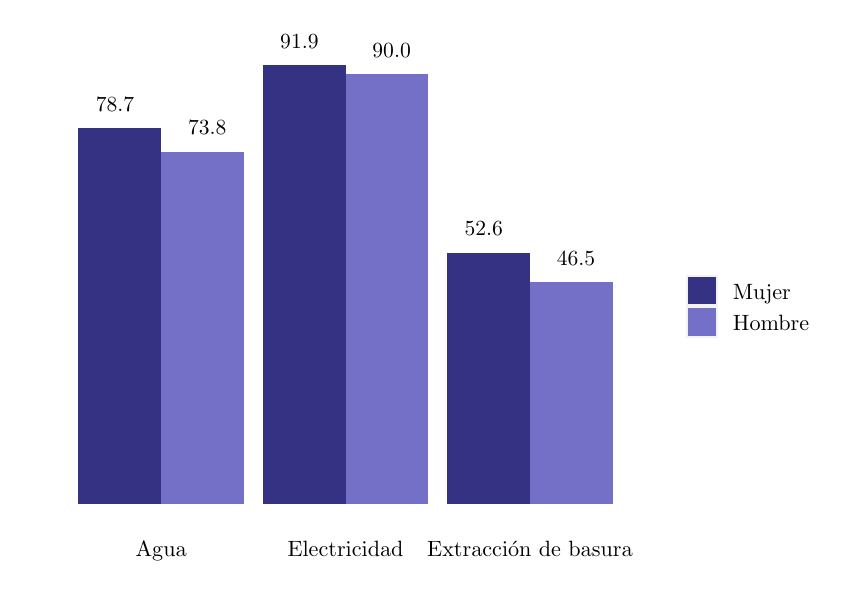
\begin{tikzpicture}[x=1pt,y=1pt]% Created by tikzDevice version 0.12.4 on 2023-05-04 16:03:14
% !TEX encoding = UTF-8 Unicode
\definecolor{fillColor}{RGB}{255,255,255}
\path[use as bounding box,fill=fillColor,fill opacity=0.00] (0,0) rectangle (289.08,198.74);
\begin{scope}
\path[clip] (  0.00,  0.00) rectangle (289.08,198.74);
\definecolor{drawColor}{RGB}{255,255,255}
\definecolor{fillColor}{RGB}{255,255,255}

\path[draw=drawColor,line width= 0.6pt,line join=round,line cap=round,fill=fillColor] (  0.00,  0.00) rectangle (289.08,198.74);
\end{scope}
\begin{scope}
\path[clip] (  0.00,  0.00) rectangle (289.08,198.74);
\definecolor{fillColor}{RGB}{54,50,131}

\path[fill=fillColor] ( 18.24, 26.74) rectangle ( 48.23,162.52);
\definecolor{fillColor}{RGB}{116,112,200}

\path[fill=fillColor] ( 48.23, 26.74) rectangle ( 78.21,153.95);
\definecolor{fillColor}{RGB}{54,50,131}

\path[fill=fillColor] (151.50, 26.74) rectangle (181.48,117.43);
\definecolor{fillColor}{RGB}{116,112,200}

\path[fill=fillColor] (181.48, 26.74) rectangle (211.46,106.87);
\definecolor{fillColor}{RGB}{54,50,131}

\path[fill=fillColor] ( 84.87, 26.74) rectangle (114.85,185.31);
\definecolor{fillColor}{RGB}{116,112,200}

\path[fill=fillColor] (114.85, 26.74) rectangle (144.83,181.97);
\definecolor{drawColor}{RGB}{0,0,0}

\node[text=drawColor,anchor=base,inner sep=0pt, outer sep=0pt, scale=  0.78] at ( 31.57,168.58) {78.7};

\node[text=drawColor,anchor=base,inner sep=0pt, outer sep=0pt, scale=  0.78] at ( 64.88,160.02) {73.8};

\node[text=drawColor,anchor=base,inner sep=0pt, outer sep=0pt, scale=  0.78] at (164.82,123.50) {52.6};

\node[text=drawColor,anchor=base,inner sep=0pt, outer sep=0pt, scale=  0.78] at (198.14,112.94) {46.5};

\node[text=drawColor,anchor=base,inner sep=0pt, outer sep=0pt, scale=  0.78] at ( 98.20,191.38) {91.9};

\node[text=drawColor,anchor=base,inner sep=0pt, outer sep=0pt, scale=  0.78] at (131.51,188.04) {90.0};
\end{scope}
\begin{scope}
\path[clip] (  0.00,  0.00) rectangle (289.08,198.74);
\definecolor{drawColor}{RGB}{0,0,0}

\node[text=drawColor,anchor=base,inner sep=0pt, outer sep=0pt, scale=  0.80] at ( 48.23,  7.60) {Agua};

\node[text=drawColor,anchor=base,inner sep=0pt, outer sep=0pt, scale=  0.80] at (114.85,  7.60) {Electricidad};

\node[text=drawColor,anchor=base,inner sep=0pt, outer sep=0pt, scale=  0.80] at (181.48,  7.60) {Extracción de basura};
\end{scope}
\begin{scope}
\path[clip] (  0.00,  0.00) rectangle (289.08,198.74);
\definecolor{fillColor}{RGB}{255,255,255}

\path[fill=fillColor] (232.46, 81.17) rectangle (283.58,130.88);
\end{scope}
\begin{scope}
\path[clip] (  0.00,  0.00) rectangle (289.08,198.74);
\definecolor{fillColor}{gray}{0.95}

\path[fill=fillColor] (237.96, 98.05) rectangle (249.34,109.43);
\end{scope}
\begin{scope}
\path[clip] (  0.00,  0.00) rectangle (289.08,198.74);
\definecolor{fillColor}{RGB}{54,50,131}

\path[fill=fillColor] (238.62, 98.71) rectangle (248.67,108.77);
\end{scope}
\begin{scope}
\path[clip] (  0.00,  0.00) rectangle (289.08,198.74);
\definecolor{fillColor}{gray}{0.95}

\path[fill=fillColor] (237.96, 86.67) rectangle (249.34, 98.05);
\end{scope}
\begin{scope}
\path[clip] (  0.00,  0.00) rectangle (289.08,198.74);
\definecolor{fillColor}{RGB}{116,112,200}

\path[fill=fillColor] (238.62, 87.33) rectangle (248.67, 97.39);
\end{scope}
\begin{scope}
\path[clip] (  0.00,  0.00) rectangle (289.08,198.74);
\definecolor{drawColor}{RGB}{0,0,0}

\node[text=drawColor,anchor=base west,inner sep=0pt, outer sep=0pt, scale=  0.80] at (254.84,100.62) {Mujer};
\end{scope}
\begin{scope}
\path[clip] (  0.00,  0.00) rectangle (289.08,198.74);
\definecolor{drawColor}{RGB}{0,0,0}

\node[text=drawColor,anchor=base west,inner sep=0pt, outer sep=0pt, scale=  0.80] at (254.84, 89.23) {Hombre};
\end{scope}
\end{tikzpicture}}{INE - ENEI 2022}{}

\cajita{Jefatura de hogar por sexo, según dominio de estudio }{En Guatemala, para 2022 el 40.7\% de jefaturas de hogar estaban ocupadas hombres en el dominio rural nacional. El 18.0\% de jefaturas fueron ocupadas por hombres en el resto urbano, y el 14.2\% por mujeres en el dominio rural nacional. }{Jefatura de hogar por sexo, según dominio de estudio (porcentaje)}{República de Guatemala, Instituto Nacional de Estadística}{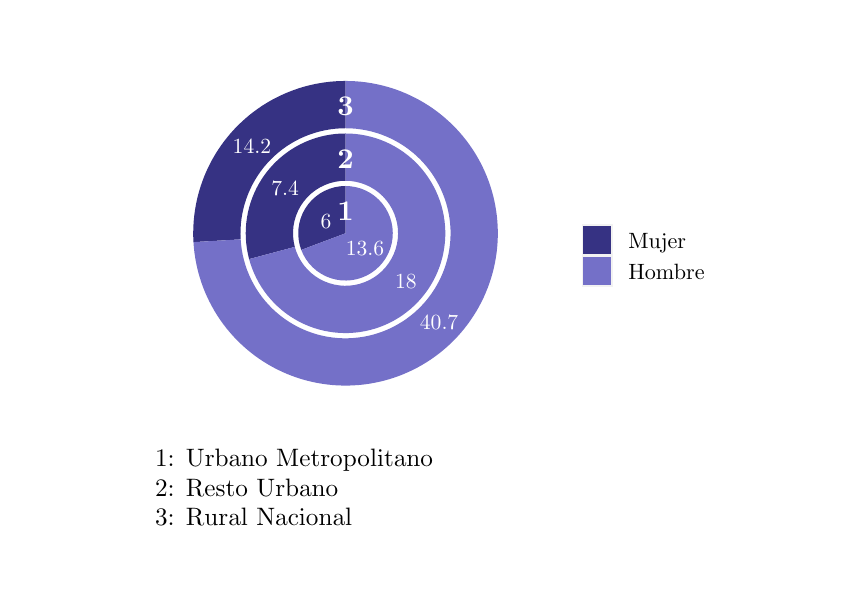
\begin{tikzpicture}[x=1pt,y=1pt]% Created by tikzDevice version 0.12.4 on 2023-05-04 16:13:12
% !TEX encoding = UTF-8 Unicode
\definecolor{fillColor}{RGB}{255,255,255}
\path[use as bounding box,fill=fillColor,fill opacity=0.00] (0,0) rectangle (289.08,198.74);
\begin{scope}
\path[clip] (  0.00,  0.00) rectangle (289.08,198.74);
\definecolor{drawColor}{RGB}{255,255,255}
\definecolor{fillColor}{RGB}{255,255,255}

\path[draw=drawColor,line width= 0.6pt,line join=round,line cap=round,fill=fillColor] ( 37.81,  0.00) rectangle (251.27,198.74);
\end{scope}
\begin{scope}
\path[clip] (  0.00,  0.00) rectangle (289.08,198.74);
\definecolor{fillColor}{RGB}{54,50,131}

\path[fill=fillColor] (114.85,124.45) --
	(114.85,126.34) --
	(114.85,128.24) --
	(114.85,130.14) --
	(114.85,132.04) --
	(114.85,133.93) --
	(114.85,135.83) --
	(114.85,137.73) --
	(114.85,139.63) --
	(114.85,141.53) --
	(112.92,141.42) --
	(111.01,141.09) --
	(109.15,140.54) --
	(107.36,139.79) --
	(105.67,138.85) --
	(104.10,137.71) --
	(102.66,136.41) --
	(101.38,134.95) --
	(100.28,133.36) --
	( 99.36,131.65) --
	( 98.65,129.85) --
	( 98.14,127.97) --
	( 97.85,126.06) --
	( 97.78,124.12) --
	( 97.92,122.19) --
	( 98.29,120.28) --
	( 98.86,118.43) --
	(100.64,119.10) --
	(102.42,119.77) --
	(104.19,120.44) --
	(105.97,121.11) --
	(107.75,121.77) --
	(109.52,122.44) --
	(111.30,123.11) --
	(113.08,123.78) --
	(114.85,124.45) --
	(114.85,124.45) --
	cycle;

\path[fill=fillColor] (114.85,143.42) --
	(114.85,145.32) --
	(114.85,147.22) --
	(114.85,149.12) --
	(114.85,151.02) --
	(114.85,152.91) --
	(114.85,154.81) --
	(114.85,156.71) --
	(114.85,158.61) --
	(114.85,160.50) --
	(112.97,160.46) --
	(111.08,160.31) --
	(109.21,160.06) --
	(107.36,159.72) --
	(105.52,159.28) --
	(103.71,158.74) --
	(101.93,158.11) --
	(100.18,157.39) --
	( 98.48,156.57) --
	( 96.82,155.67) --
	( 95.21,154.69) --
	( 93.66,153.62) --
	( 92.16,152.47) --
	( 90.72,151.24) --
	( 89.35,149.94) --
	( 88.05,148.57) --
	( 86.83,147.14) --
	( 85.68,145.64) --
	( 84.61,144.08) --
	( 83.62,142.47) --
	( 82.72,140.81) --
	( 81.91,139.11) --
	( 81.19,137.36) --
	( 80.56,135.58) --
	( 80.02,133.77) --
	( 79.58,131.94) --
	( 79.24,130.08) --
	( 78.99,128.21) --
	( 78.84,126.33) --
	( 78.79,124.44) --
	( 78.84,122.55) --
	( 78.99,120.67) --
	( 79.24,118.80) --
	( 79.58,116.94) --
	( 80.02,115.11) --
	( 81.86,115.60) --
	( 83.69,116.09) --
	( 85.52,116.58) --
	( 87.36,117.07) --
	( 89.19,117.56) --
	( 91.02,118.06) --
	( 92.86,118.55) --
	( 94.69,119.04) --
	( 96.52,119.53) --
	( 96.12,121.42) --
	( 95.91,123.34) --
	( 95.89,125.27) --
	( 96.07,127.19) --
	( 96.45,129.09) --
	( 97.02,130.93) --
	( 97.77,132.71) --
	( 98.70,134.41) --
	( 99.80,136.00) --
	(101.05,137.47) --
	(102.44,138.80) --
	(103.97,139.99) --
	(105.60,141.02) --
	(107.34,141.87) --
	(109.15,142.55) --
	(111.01,143.03) --
	(112.92,143.33) --
	(114.85,143.42) --
	cycle;

\path[fill=fillColor] (114.85,162.40) --
	(114.85,164.30) --
	(114.85,166.20) --
	(114.85,168.10) --
	(114.85,169.99) --
	(114.85,171.89) --
	(114.85,173.79) --
	(114.85,175.69) --
	(114.85,177.59) --
	(114.85,179.48) --
	(112.99,179.45) --
	(111.12,179.36) --
	(109.26,179.20) --
	(107.40,178.98) --
	(105.56,178.69) --
	(103.72,178.35) --
	(101.90,177.94) --
	(100.09,177.47) --
	( 98.30,176.94) --
	( 96.53,176.34) --
	( 94.78,175.69) --
	( 93.05,174.98) --
	( 91.35,174.21) --
	( 89.68,173.39) --
	( 88.03,172.51) --
	( 86.42,171.57) --
	( 84.83,170.58) --
	( 83.29,169.53) --
	( 81.77,168.43) --
	( 80.30,167.29) --
	( 78.87,166.09) --
	( 77.47,164.84) --
	( 76.13,163.55) --
	( 74.82,162.22) --
	( 73.56,160.84) --
	( 72.35,159.41) --
	( 71.19,157.95) --
	( 70.08,156.45) --
	( 69.02,154.91) --
	( 68.01,153.34) --
	( 67.06,151.73) --
	( 66.16,150.10) --
	( 65.32,148.43) --
	( 64.53,146.74) --
	( 63.80,145.02) --
	( 63.14,143.27) --
	( 62.53,141.51) --
	( 61.98,139.72) --
	( 61.49,137.92) --
	( 61.06,136.10) --
	( 60.70,134.27) --
	( 60.40,132.43) --
	( 60.16,130.57) --
	( 59.98,128.71) --
	( 59.87,126.85) --
	( 59.82,124.98) --
	( 59.83,123.11) --
	( 59.91,121.25) --
	( 61.80,121.36) --
	( 63.70,121.47) --
	( 65.59,121.58) --
	( 67.49,121.69) --
	( 69.38,121.80) --
	( 71.28,121.91) --
	( 73.17,122.02) --
	( 75.07,122.13) --
	( 76.96,122.24) --
	( 76.90,124.11) --
	( 76.93,125.99) --
	( 77.05,127.86) --
	( 77.26,129.72) --
	( 77.57,131.57) --
	( 77.97,133.40) --
	( 78.45,135.21) --
	( 79.03,136.99) --
	( 79.69,138.74) --
	( 80.44,140.46) --
	( 81.27,142.14) --
	( 82.18,143.77) --
	( 83.18,145.36) --
	( 84.25,146.90) --
	( 85.39,148.38) --
	( 86.61,149.80) --
	( 87.90,151.17) --
	( 89.25,152.46) --
	( 90.66,153.69) --
	( 92.13,154.85) --
	( 93.66,155.94) --
	( 95.24,156.94) --
	( 96.87,157.87) --
	( 98.54,158.72) --
	(100.25,159.48) --
	(102.00,160.16) --
	(103.77,160.75) --
	(105.58,161.25) --
	(107.41,161.66) --
	(109.25,161.99) --
	(111.11,162.22) --
	(112.98,162.36) --
	(114.85,162.40) --
	cycle;
\definecolor{fillColor}{RGB}{116,112,200}

\path[fill=fillColor] (114.85,124.45) --
	(113.08,123.78) --
	(111.30,123.11) --
	(109.52,122.44) --
	(107.75,121.77) --
	(105.97,121.11) --
	(104.19,120.44) --
	(102.42,119.77) --
	(100.64,119.10) --
	( 98.86,118.43) --
	( 99.63,116.69) --
	(100.59,115.04) --
	(101.73,113.51) --
	(103.03,112.12) --
	(104.47,110.88) --
	(106.05,109.81) --
	(107.73,108.92) --
	(109.51,108.22) --
	(111.35,107.73) --
	(113.23,107.44) --
	(115.14,107.37) --
	(117.04,107.50) --
	(118.91,107.85) --
	(120.73,108.41) --
	(122.48,109.16) --
	(124.14,110.11) --
	(125.67,111.23) --
	(127.08,112.52) --
	(128.33,113.95) --
	(129.42,115.52) --
	(130.32,117.20) --
	(131.03,118.97) --
	(131.54,120.80) --
	(131.84,122.68) --
	(131.93,124.59) --
	(131.81,126.49) --
	(131.48,128.36) --
	(130.94,130.19) --
	(130.20,131.95) --
	(129.27,133.61) --
	(128.16,135.16) --
	(126.88,136.57) --
	(125.46,137.84) --
	(123.90,138.93) --
	(122.23,139.85) --
	(120.47,140.58) --
	(118.63,141.10) --
	(116.76,141.42) --
	(114.85,141.53) --
	(114.85,139.63) --
	(114.85,137.73) --
	(114.85,135.83) --
	(114.85,133.93) --
	(114.85,132.04) --
	(114.85,130.14) --
	(114.85,128.24) --
	(114.85,126.34) --
	(114.85,124.45) --
	(114.85,124.45) --
	cycle;

\path[fill=fillColor] ( 96.52,119.53) --
	( 94.69,119.04) --
	( 92.86,118.55) --
	( 91.02,118.06) --
	( 89.19,117.56) --
	( 87.36,117.07) --
	( 85.52,116.58) --
	( 83.69,116.09) --
	( 81.86,115.60) --
	( 80.02,115.11) --
	( 80.55,113.32) --
	( 81.18,111.56) --
	( 81.89,109.83) --
	( 82.69,108.15) --
	( 83.57,106.51) --
	( 84.54,104.91) --
	( 85.59,103.37) --
	( 86.72,101.88) --
	( 87.93,100.46) --
	( 89.20, 99.10) --
	( 90.55, 97.81) --
	( 91.96, 96.58) --
	( 93.43, 95.44) --
	( 94.96, 94.37) --
	( 96.54, 93.38) --
	( 98.17, 92.47) --
	( 99.85, 91.65) --
	(101.57, 90.92) --
	(103.32, 90.28) --
	(105.10, 89.73) --
	(106.91, 89.27) --
	(108.74, 88.91) --
	(110.59, 88.64) --
	(112.44, 88.47) --
	(114.31, 88.39) --
	(116.17, 88.41) --
	(118.04, 88.53) --
	(119.89, 88.74) --
	(121.73, 89.05) --
	(123.55, 89.45) --
	(125.35, 89.95) --
	(127.12, 90.54) --
	(128.86, 91.22) --
	(130.56, 91.99) --
	(132.22, 92.84) --
	(133.83, 93.78) --
	(135.39, 94.80) --
	(136.89, 95.91) --
	(138.34, 97.08) --
	(139.72, 98.34) --
	(141.04, 99.66) --
	(142.29,101.05) --
	(143.46,102.50) --
	(144.56,104.01) --
	(145.58,105.57) --
	(146.51,107.18) --
	(147.36,108.84) --
	(148.13,110.55) --
	(148.80,112.29) --
	(149.38,114.06) --
	(149.88,115.86) --
	(150.27,117.68) --
	(150.57,119.52) --
	(150.78,121.38) --
	(150.89,123.24) --
	(150.91,125.11) --
	(150.82,126.97) --
	(150.64,128.83) --
	(150.37,130.67) --
	(150.00,132.50) --
	(149.54,134.31) --
	(148.98,136.09) --
	(148.33,137.84) --
	(147.59,139.55) --
	(146.77,141.23) --
	(145.86,142.85) --
	(144.86,144.43) --
	(143.79,145.96) --
	(142.64,147.43) --
	(141.41,148.83) --
	(140.12,150.18) --
	(138.75,151.45) --
	(137.32,152.65) --
	(135.83,153.77) --
	(134.29,154.82) --
	(132.69,155.78) --
	(131.05,156.66) --
	(129.36,157.46) --
	(127.63,158.16) --
	(125.87,158.78) --
	(124.08,159.30) --
	(122.26,159.73) --
	(120.43,160.07) --
	(118.58,160.31) --
	(116.72,160.46) --
	(114.85,160.50) --
	(114.85,158.61) --
	(114.85,156.71) --
	(114.85,154.81) --
	(114.85,152.91) --
	(114.85,151.02) --
	(114.85,149.12) --
	(114.85,147.22) --
	(114.85,145.32) --
	(114.85,143.42) --
	(116.73,143.33) --
	(118.58,143.05) --
	(120.40,142.59) --
	(122.17,141.96) --
	(123.86,141.15) --
	(125.47,140.18) --
	(126.97,139.05) --
	(128.35,137.79) --
	(129.60,136.39) --
	(130.71,134.87) --
	(131.66,133.26) --
	(132.45,131.56) --
	(133.07,129.78) --
	(133.50,127.96) --
	(133.76,126.10) --
	(133.83,124.23) --
	(133.72,122.35) --
	(133.42,120.50) --
	(132.94,118.69) --
	(132.28,116.93) --
	(131.45,115.25) --
	(130.46,113.65) --
	(129.32,112.16) --
	(128.04,110.79) --
	(126.63,109.56) --
	(125.10,108.47) --
	(123.47,107.54) --
	(121.76,106.77) --
	(119.98,106.17) --
	(118.15,105.76) --
	(116.29,105.52) --
	(114.41,105.47) --
	(112.54,105.61) --
	(110.69,105.93) --
	(108.89,106.43) --
	(107.14,107.11) --
	(105.46,107.95) --
	(103.88,108.96) --
	(102.40,110.12) --
	(101.05,111.42) --
	( 99.83,112.85) --
	( 98.76,114.39) --
	( 97.85,116.02) --
	( 97.10,117.74) --
	( 96.52,119.53) --
	cycle;

\path[fill=fillColor] ( 76.96,122.24) --
	( 75.07,122.13) --
	( 73.17,122.02) --
	( 71.28,121.91) --
	( 69.38,121.80) --
	( 67.49,121.69) --
	( 65.59,121.58) --
	( 63.70,121.47) --
	( 61.80,121.36) --
	( 59.91,121.25) --
	( 60.05,119.38) --
	( 60.25,117.53) --
	( 60.52,115.68) --
	( 60.85,113.83) --
	( 61.24,112.01) --
	( 61.69,110.19) --
	( 62.21,108.40) --
	( 62.78,106.62) --
	( 63.42,104.86) --
	( 64.11,103.12) --
	( 64.87,101.41) --
	( 65.68, 99.73) --
	( 66.55, 98.07) --
	( 67.47, 96.44) --
	( 68.45, 94.85) --
	( 69.48, 93.29) --
	( 70.56, 91.77) --
	( 71.70, 90.28) --
	( 72.89, 88.84) --
	( 74.12, 87.43) --
	( 75.40, 86.07) --
	( 76.73, 84.75) --
	( 78.10, 83.48) --
	( 79.51, 82.26) --
	( 80.96, 81.08) --
	( 82.45, 79.95) --
	( 83.98, 78.88) --
	( 85.55, 77.86) --
	( 87.15, 76.89) --
	( 88.78, 75.97) --
	( 90.44, 75.12) --
	( 92.13, 74.32) --
	( 93.85, 73.57) --
	( 95.59, 72.89) --
	( 97.35, 72.26) --
	( 99.13, 71.70) --
	(100.93, 71.20) --
	(102.75, 70.75) --
	(104.58, 70.37) --
	(106.42, 70.06) --
	(108.27, 69.80) --
	(110.13, 69.61) --
	(112.00, 69.48) --
	(113.87, 69.42) --
	(115.74, 69.41) --
	(117.61, 69.48) --
	(119.47, 69.60) --
	(121.33, 69.79) --
	(123.19, 70.04) --
	(125.03, 70.36) --
	(126.86, 70.73) --
	(128.68, 71.17) --
	(130.48, 71.67) --
	(132.26, 72.23) --
	(134.03, 72.85) --
	(135.77, 73.54) --
	(137.48, 74.28) --
	(139.18, 75.07) --
	(140.84, 75.93) --
	(142.47, 76.84) --
	(144.07, 77.80) --
	(145.64, 78.82) --
	(147.17, 79.90) --
	(148.67, 81.02) --
	(150.12, 82.19) --
	(151.54, 83.41) --
	(152.91, 84.68) --
	(154.24, 86.00) --
	(155.52, 87.36) --
	(156.76, 88.76) --
	(157.94, 90.21) --
	(159.08, 91.69) --
	(160.17, 93.21) --
	(161.20, 94.77) --
	(162.19, 96.36) --
	(163.11, 97.98) --
	(163.98, 99.64) --
	(164.80,101.32) --
	(165.55,103.03) --
	(166.25,104.77) --
	(166.89,106.52) --
	(167.47,108.30) --
	(167.99,110.10) --
	(168.44,111.91) --
	(168.84,113.74) --
	(169.17,115.58) --
	(169.44,117.43) --
	(169.65,119.29) --
	(169.79,121.15) --
	(169.87,123.02) --
	(169.89,124.89) --
	(169.84,126.76) --
	(169.73,128.62) --
	(169.56,130.49) --
	(169.32,132.34) --
	(169.02,134.19) --
	(168.66,136.02) --
	(168.24,137.84) --
	(167.75,139.65) --
	(167.20,141.43) --
	(166.60,143.20) --
	(165.93,144.95) --
	(165.20,146.67) --
	(164.42,148.37) --
	(163.58,150.04) --
	(162.68,151.68) --
	(161.73,153.29) --
	(160.72,154.86) --
	(159.66,156.40) --
	(158.55,157.91) --
	(157.39,159.37) --
	(156.18,160.80) --
	(154.92,162.18) --
	(153.61,163.52) --
	(152.26,164.81) --
	(150.87,166.06) --
	(149.44,167.26) --
	(147.96,168.41) --
	(146.45,169.51) --
	(144.90,170.56) --
	(143.32,171.55) --
	(141.70,172.49) --
	(140.05,173.37) --
	(138.38,174.20) --
	(136.67,174.97) --
	(134.95,175.68) --
	(133.19,176.34) --
	(131.42,176.93) --
	(129.63,177.46) --
	(127.82,177.93) --
	(125.99,178.34) --
	(124.16,178.69) --
	(122.31,178.98) --
	(120.45,179.20) --
	(118.59,179.36) --
	(116.72,179.45) --
	(114.85,179.48) --
	(114.85,177.59) --
	(114.85,175.69) --
	(114.85,173.79) --
	(114.85,171.89) --
	(114.85,169.99) --
	(114.85,168.10) --
	(114.85,166.20) --
	(114.85,164.30) --
	(114.85,162.40) --
	(116.73,162.36) --
	(118.61,162.22) --
	(120.47,161.98) --
	(122.32,161.66) --
	(124.15,161.25) --
	(125.96,160.74) --
	(127.75,160.15) --
	(129.50,159.46) --
	(131.21,158.70) --
	(132.89,157.84) --
	(134.52,156.91) --
	(136.10,155.90) --
	(137.63,154.81) --
	(139.11,153.64) --
	(140.52,152.41) --
	(141.88,151.10) --
	(143.16,149.73) --
	(144.38,148.30) --
	(145.52,146.81) --
	(146.59,145.26) --
	(147.58,143.67) --
	(148.49,142.02) --
	(149.32,140.34) --
	(150.07,138.61) --
	(150.73,136.85) --
	(151.30,135.06) --
	(151.78,133.24) --
	(152.17,131.41) --
	(152.47,129.55) --
	(152.67,127.68) --
	(152.79,125.81) --
	(152.81,123.93) --
	(152.73,122.05) --
	(152.57,120.18) --
	(152.31,118.32) --
	(151.96,116.47) --
	(151.52,114.64) --
	(150.99,112.84) --
	(150.37,111.07) --
	(149.67,109.32) --
	(148.88,107.62) --
	(148.00,105.96) --
	(147.05,104.34) --
	(146.01,102.77) --
	(144.90,101.25) --
	(143.72, 99.79) --
	(142.46, 98.40) --
	(141.14, 97.06) --
	(139.75, 95.79) --
	(138.30, 94.60) --
	(136.80, 93.47) --
	(135.24, 92.43) --
	(133.63, 91.46) --
	(131.97, 90.57) --
	(130.27, 89.76) --
	(128.54, 89.04) --
	(126.77, 88.41) --
	(124.97, 87.86) --
	(123.15, 87.41) --
	(121.30, 87.04) --
	(119.44, 86.77) --
	(117.57, 86.59) --
	(115.70, 86.50) --
	(113.82, 86.50) --
	(111.94, 86.60) --
	(110.07, 86.79) --
	(108.21, 87.07) --
	(106.37, 87.45) --
	(104.55, 87.91) --
	(102.76, 88.47) --
	(100.99, 89.11) --
	( 99.26, 89.84) --
	( 97.56, 90.65) --
	( 95.91, 91.55) --
	( 94.31, 92.53) --
	( 92.75, 93.58) --
	( 91.25, 94.72) --
	( 89.81, 95.92) --
	( 88.43, 97.19) --
	( 87.11, 98.54) --
	( 85.87, 99.94) --
	( 84.69,101.41) --
	( 83.58,102.93) --
	( 82.56,104.50) --
	( 81.61,106.12) --
	( 80.74,107.79) --
	( 79.96,109.50) --
	( 79.26,111.24) --
	( 78.66,113.02) --
	( 78.13,114.83) --
	( 77.70,116.66) --
	( 77.36,118.51) --
	( 77.12,120.37) --
	( 76.96,122.24) --
	cycle;
\definecolor{drawColor}{RGB}{255,255,255}

\node[text=drawColor,anchor=base,inner sep=0pt, outer sep=0pt, scale=  0.78] at (107.83,126.27) {6};

\node[text=drawColor,anchor=base,inner sep=0pt, outer sep=0pt, scale=  0.78] at ( 93.02,138.16) {7.4};

\node[text=drawColor,anchor=base,inner sep=0pt, outer sep=0pt, scale=  0.78] at ( 81.03,153.32) {14.2};

\node[text=drawColor,anchor=base,inner sep=0pt, outer sep=0pt, scale=  0.78] at (121.87,116.55) {13.6};

\node[text=drawColor,anchor=base,inner sep=0pt, outer sep=0pt, scale=  0.78] at (136.69,104.66) {18};

\node[text=drawColor,anchor=base,inner sep=0pt, outer sep=0pt, scale=  0.78] at (148.67, 89.50) {40.7};

\node[text=drawColor,anchor=base,inner sep=0pt, outer sep=0pt, scale=  1.03] at (114.85,128.94) {\bfseries 1};

\node[text=drawColor,anchor=base,inner sep=0pt, outer sep=0pt, scale=  1.03] at (114.85,147.92) {\bfseries 2};

\node[text=drawColor,anchor=base,inner sep=0pt, outer sep=0pt, scale=  1.03] at (114.85,166.90) {\bfseries 3};
\end{scope}
\begin{scope}
\path[clip] (  0.00,  0.00) rectangle (289.08,198.74);
\definecolor{fillColor}{RGB}{255,255,255}

\path[fill=fillColor] (194.65, 99.59) rectangle (245.77,149.30);
\end{scope}
\begin{scope}
\path[clip] (  0.00,  0.00) rectangle (289.08,198.74);
\definecolor{fillColor}{gray}{0.95}

\path[fill=fillColor] (200.15,116.47) rectangle (211.53,127.85);
\end{scope}
\begin{scope}
\path[clip] (  0.00,  0.00) rectangle (289.08,198.74);
\definecolor{fillColor}{RGB}{54,50,131}

\path[fill=fillColor] (200.81,117.13) rectangle (210.87,127.19);
\end{scope}
\begin{scope}
\path[clip] (  0.00,  0.00) rectangle (289.08,198.74);
\definecolor{fillColor}{gray}{0.95}

\path[fill=fillColor] (200.15,105.09) rectangle (211.53,116.47);
\end{scope}
\begin{scope}
\path[clip] (  0.00,  0.00) rectangle (289.08,198.74);
\definecolor{fillColor}{RGB}{116,112,200}

\path[fill=fillColor] (200.81,105.75) rectangle (210.87,115.81);
\end{scope}
\begin{scope}
\path[clip] (  0.00,  0.00) rectangle (289.08,198.74);
\definecolor{drawColor}{RGB}{0,0,0}

\node[text=drawColor,anchor=base west,inner sep=0pt, outer sep=0pt, scale=  0.80] at (217.03,119.04) {Mujer};
\end{scope}
\begin{scope}
\path[clip] (  0.00,  0.00) rectangle (289.08,198.74);
\definecolor{drawColor}{RGB}{0,0,0}

\node[text=drawColor,anchor=base west,inner sep=0pt, outer sep=0pt, scale=  0.80] at (217.03,107.65) {Hombre};
\end{scope}
\begin{scope}
\path[clip] (  0.00,  0.00) rectangle (289.08,198.74);
\definecolor{drawColor}{RGB}{0,0,0}

\node[text=drawColor,anchor=base west,inner sep=0pt, outer sep=0pt, scale=  0.91] at ( 46.06, 40.29) {1: Urbano Metropolitano};

\node[text=drawColor,anchor=base west,inner sep=0pt, outer sep=0pt, scale=  0.91] at ( 46.06, 29.49) {2: Resto Urbano};

\node[text=drawColor,anchor=base west,inner sep=0pt, outer sep=0pt, scale=  0.91] at ( 46.06, 18.69) {3: Rural Nacional};

\node[text=drawColor,anchor=base west,inner sep=0pt, outer sep=0pt, scale=  0.91] at ( 46.06,  7.89) {};
\end{scope}
\end{tikzpicture}}{INE - ENEI 2022}{}

\cajita{Jefatura de hogar por sexo, según estado conyugal }{En Guatemala, para 2022 las jefaturas de hogar según estado conyugal fueron ejercidas en 9.6\% por mujeres viudas, seguido por mujeres solteras con 6.1\% y 4.7\% por mujeres casadas. 
}{Jefatura de hogar por sexo, según estado conyugal (porcentaje)}{República de Guatemala, Instituto Nacional de Estadística}{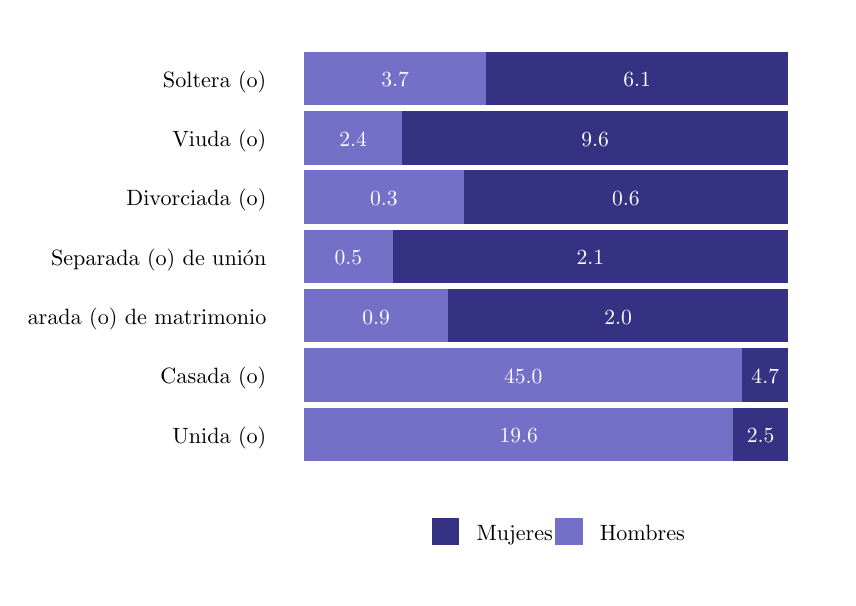
\begin{tikzpicture}[x=1pt,y=1pt]% Created by tikzDevice version 0.12.4 on 2023-05-04 15:57:46
% !TEX encoding = UTF-8 Unicode
\definecolor{fillColor}{RGB}{255,255,255}
\path[use as bounding box,fill=fillColor,fill opacity=0.00] (0,0) rectangle (289.08,198.74);
\begin{scope}
\path[clip] (  0.00,  0.00) rectangle (289.08,198.74);
\definecolor{drawColor}{RGB}{255,255,255}
\definecolor{fillColor}{RGB}{255,255,255}

\path[draw=drawColor,line width= 0.6pt,line join=round,line cap=round,fill=fillColor] (  0.00,  0.00) rectangle (289.08,198.74);
\end{scope}
\begin{scope}
\path[clip] (  0.00,  0.00) rectangle (289.08,198.74);
\definecolor{fillColor}{RGB}{54,50,131}

\path[fill=fillColor] (254.93, 42.10) rectangle (274.84, 61.39);

\path[fill=fillColor] (258.23, 63.54) rectangle (274.84, 82.83);

\path[fill=fillColor] (151.87, 84.98) rectangle (274.84,104.27);

\path[fill=fillColor] (131.90,106.41) rectangle (274.84,125.71);

\path[fill=fillColor] (157.51,127.85) rectangle (274.84,147.15);

\path[fill=fillColor] (135.29,149.29) rectangle (274.84,168.59);

\path[fill=fillColor] (165.59,170.73) rectangle (274.84,190.03);
\definecolor{fillColor}{RGB}{116,112,200}

\path[fill=fillColor] ( 99.94, 42.10) rectangle (254.93, 61.39);

\path[fill=fillColor] ( 99.94, 63.54) rectangle (258.23, 82.83);

\path[fill=fillColor] ( 99.94, 84.98) rectangle (151.87,104.27);

\path[fill=fillColor] ( 99.94,106.41) rectangle (131.90,125.71);

\path[fill=fillColor] ( 99.94,127.85) rectangle (157.51,147.15);

\path[fill=fillColor] ( 99.94,149.29) rectangle (135.29,168.59);

\path[fill=fillColor] ( 99.94,170.73) rectangle (165.59,190.03);
\definecolor{drawColor}{RGB}{255,255,255}

\node[text=drawColor,anchor=base,inner sep=0pt, outer sep=0pt, scale=  0.78] at (264.88, 48.71) {2.5};

\node[text=drawColor,anchor=base,inner sep=0pt, outer sep=0pt, scale=  0.78] at (266.53, 70.15) {4.7};

\node[text=drawColor,anchor=base,inner sep=0pt, outer sep=0pt, scale=  0.78] at (213.35, 91.59) {2.0};

\node[text=drawColor,anchor=base,inner sep=0pt, outer sep=0pt, scale=  0.78] at (203.37,113.03) {2.1};

\node[text=drawColor,anchor=base,inner sep=0pt, outer sep=0pt, scale=  0.78] at (216.17,134.47) {0.6};

\node[text=drawColor,anchor=base,inner sep=0pt, outer sep=0pt, scale=  0.78] at (205.06,155.91) {9.6};

\node[text=drawColor,anchor=base,inner sep=0pt, outer sep=0pt, scale=  0.78] at (220.21,177.35) {6.1};

\node[text=drawColor,anchor=base,inner sep=0pt, outer sep=0pt, scale=  0.78] at (177.43, 48.71) {19.6};

\node[text=drawColor,anchor=base,inner sep=0pt, outer sep=0pt, scale=  0.78] at (179.09, 70.15) {45.0};

\node[text=drawColor,anchor=base,inner sep=0pt, outer sep=0pt, scale=  0.78] at (125.90, 91.59) {0.9};

\node[text=drawColor,anchor=base,inner sep=0pt, outer sep=0pt, scale=  0.78] at (115.92,113.03) {0.5};

\node[text=drawColor,anchor=base,inner sep=0pt, outer sep=0pt, scale=  0.78] at (128.73,134.47) {0.3};

\node[text=drawColor,anchor=base,inner sep=0pt, outer sep=0pt, scale=  0.78] at (117.62,155.91) {2.4};

\node[text=drawColor,anchor=base,inner sep=0pt, outer sep=0pt, scale=  0.78] at (132.77,177.35) {3.7};
\end{scope}
\begin{scope}
\path[clip] (  0.00,  0.00) rectangle (289.08,198.74);
\definecolor{drawColor}{RGB}{0,0,0}

\node[text=drawColor,anchor=base east,inner sep=0pt, outer sep=0pt, scale=  0.80] at ( 86.25, 48.62) {Unida (o)};

\node[text=drawColor,anchor=base east,inner sep=0pt, outer sep=0pt, scale=  0.80] at ( 86.25, 70.06) {Casada (o)};

\node[text=drawColor,anchor=base east,inner sep=0pt, outer sep=0pt, scale=  0.80] at ( 86.25, 91.50) {Separada (o) de matrimonio};

\node[text=drawColor,anchor=base east,inner sep=0pt, outer sep=0pt, scale=  0.80] at ( 86.25,112.94) {Separada (o) de unión};

\node[text=drawColor,anchor=base east,inner sep=0pt, outer sep=0pt, scale=  0.80] at ( 86.25,134.37) {Divorciada (o)};

\node[text=drawColor,anchor=base east,inner sep=0pt, outer sep=0pt, scale=  0.80] at ( 86.25,155.81) {Viuda (o)};

\node[text=drawColor,anchor=base east,inner sep=0pt, outer sep=0pt, scale=  0.80] at ( 86.25,177.25) {Soltera (o)};
\end{scope}
\begin{scope}
\path[clip] (  0.00,  0.00) rectangle (289.08,198.74);
\definecolor{fillColor}{RGB}{255,255,255}

\path[fill=fillColor] (139.31,  5.50) rectangle (235.47, 27.88);
\end{scope}
\begin{scope}
\path[clip] (  0.00,  0.00) rectangle (289.08,198.74);
\definecolor{fillColor}{gray}{0.95}

%\path[fill=fillColor] (150.31, 11.00) rectangle (161.69, 22.38);
\end{scope}
\begin{scope}
\path[clip] (  0.00,  0.00) rectangle (289.08,198.74);
\definecolor{fillColor}{RGB}{54,50,131}

\path[fill=fillColor] (145.97, 11.66) rectangle (156.02, 21.72); %cuadro leyenda
\end{scope}
\begin{scope}
\path[clip] (  0.00,  0.00) rectangle (289.08,198.74);
\definecolor{fillColor}{gray}{0.95}

%\path[fill=fillColor] (161.02, 11.66) rectangle (161.02, 11.66);
\end{scope}
\begin{scope}
\path[clip] (  0.00,  0.00) rectangle (289.08,198.74);
\definecolor{fillColor}{RGB}{116,112,200}

\path[fill=fillColor] (190.51, 11.66) rectangle (200.57, 21.72);
\end{scope}
\begin{scope}
\path[clip] (  0.00,  0.00) rectangle (289.08,198.74);
\definecolor{drawColor}{RGB}{0,0,0}

\node[text=drawColor,anchor=base west,inner sep=0pt, outer sep=0pt, scale=  0.80] at (162.19, 13.56) {Mujeres};
\end{scope}
\begin{scope}
\path[clip] (  0.00,  0.00) rectangle (289.08,198.74);
\definecolor{drawColor}{RGB}{0,0,0}

\node[text=drawColor,anchor=base west,inner sep=0pt, outer sep=0pt, scale=  0.80] at (206.73, 13.56) {Hombres};
\end{scope}
\end{tikzpicture}}{INE - ENEI 2022}{}

\cajita{Mujeres jefas de hogar por número de hijas(os) }{En Guatemala para el 2022, del total de jefaturas de hogar ocupadas por mujeres el 45.8\% tenían entre 1 y 3 hijas(os), el 31.8\% entre 4 y 6 hijas(os) y el 15.1\% 7 hijas(os) o más. Por el contrario el 7.2\% no tenían hijas(os). \footnote{Los resultados reportados no suman el cien por ciento debido al redondeo de los mismos.}}{Mujeres jefas de hogar por número de hijas(os) (porcentaje)}{República de Guatemala, Instituto Nacional de Estadística}{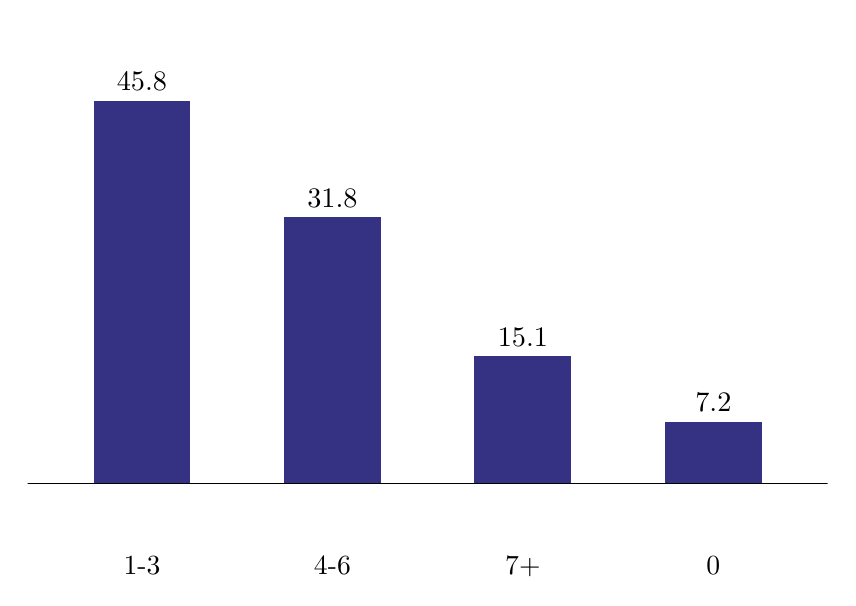
\begin{tikzpicture}[x=1pt,y=1pt]% Created by tikzDevice version 0.12.4 on 2023-05-04 16:29:24
% !TEX encoding = UTF-8 Unicode
\definecolor{fillColor}{RGB}{255,255,255}
\path[use as bounding box,fill=fillColor,fill opacity=0.00] (0,0) rectangle (289.08,198.74);
\begin{scope}
\path[clip] (  0.00,  0.00) rectangle (289.08,198.74);

\path[] (  0.00,  0.00) rectangle (289.08,198.74);
\end{scope}
\begin{scope}
\path[clip] (  0.00,  0.00) rectangle (289.08,198.74);
\definecolor{drawColor}{RGB}{54,50,131}
\definecolor{fillColor}{RGB}{54,50,131}

\path[draw=drawColor,line width= 0.6pt,fill=fillColor] ( 24.09, 34.31) rectangle ( 58.50,171.94);

\path[draw=drawColor,line width= 0.6pt,fill=fillColor] ( 92.92, 34.31) rectangle (127.33,129.87);

\path[draw=drawColor,line width= 0.6pt,fill=fillColor] (161.75, 34.31) rectangle (196.16, 79.68);

\path[draw=drawColor,line width= 0.6pt,fill=fillColor] (230.58, 34.31) rectangle (264.99, 55.94);
\definecolor{drawColor}{RGB}{0,0,0}

\path[draw=drawColor,line width= 0.1pt,line join=round] (-289.08, 34.31) -- (578.16, 34.31);

\node[text=drawColor,anchor=base,inner sep=0pt, outer sep=0pt, scale=  1.02] at ( 41.30,175.91) {45.8};

\node[text=drawColor,anchor=base,inner sep=0pt, outer sep=0pt, scale=  1.02] at (110.13,133.84) {31.8};

\node[text=drawColor,anchor=base,inner sep=0pt, outer sep=0pt, scale=  1.02] at (178.95, 83.66) {15.1};

\node[text=drawColor,anchor=base,inner sep=0pt, outer sep=0pt, scale=  1.02] at (247.78, 59.91) {7.2};

\path[] (  0.00, 27.42) rectangle (289.08,178.83);

\path[] ( 41.30, 27.42) --
	( 41.30,178.83);

\path[] (110.13, 27.42) --
	(110.13,178.83);

\path[] (178.95, 27.42) --
	(178.95,178.83);

\path[] (247.78, 27.42) --
	(247.78,178.83);

\path[] (  0.00, 27.42) rectangle (289.08,178.83);
\end{scope}
\begin{scope}
\path[clip] (  0.00,  0.00) rectangle (289.08,198.74);

\path[] (  0.00, 27.42) --
	(  0.00,178.83);
\end{scope}
\begin{scope}
\path[clip] (  0.00,  0.00) rectangle (289.08,198.74);

\path[] (  0.00, 27.42) --
	(289.08, 27.42);
\end{scope}
\begin{scope}
\path[clip] (  0.00,  0.00) rectangle (289.08,198.74);

\path[] ( 41.30, 24.67) --
	( 41.30, 27.42);

\path[] (110.13, 24.67) --
	(110.13, 27.42);

\path[] (178.95, 24.67) --
	(178.95, 27.42);

\path[] (247.78, 24.67) --
	(247.78, 27.42);
\end{scope}
\begin{scope}
\path[clip] (  0.00,  0.00) rectangle (289.08,198.74);
\definecolor{drawColor}{RGB}{0,0,0}

\node[text=drawColor,anchor=base,inner sep=0pt, outer sep=0pt, scale=  1.00] at ( 41.30,  1.32) {1-3};

\node[text=drawColor,anchor=base,inner sep=0pt, outer sep=0pt, scale=  1.00] at (110.13,  1.32) {4-6};

\node[text=drawColor,anchor=base,inner sep=0pt, outer sep=0pt, scale=  1.00] at (178.95,  1.32) {7+};

\node[text=drawColor,anchor=base,inner sep=0pt, outer sep=0pt, scale=  1.00] at (247.78,  1.32) {0};
\end{scope}
\end{tikzpicture}}{INE - ENEI 2022}{}